\documentclass{article}
\usepackage{graphicx}
\usepackage{color}
\usepackage{hyperref}
\graphicspath{ {/asay/Desktop/images/} }
\usepackage{xepersian}


\title{پاسخ تمرین شماره ۵ درس معماری کامپیوتر 
	\\
	نصب و راه اندازی
	\textcolor{red}{\lr{gem5}}}


\author{امیر حسین عاصم یوسفی \\ ۹۶۱۱۰۳۲۳}
\settextfont{B Nazanin}

\begin{document}
	\maketitle
	\section*{مستندات نصب  }
	چون از قبل این پیش نیازها نصب شده است نتیجه دستورات به صورت زیر است  : 
		\begin{center}
		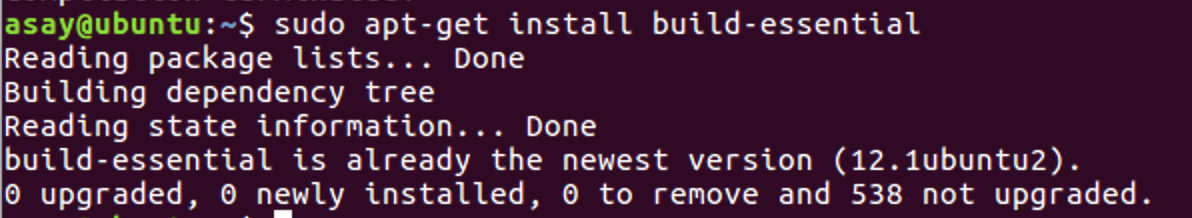
\includegraphics[width=1\textwidth]{essential}
				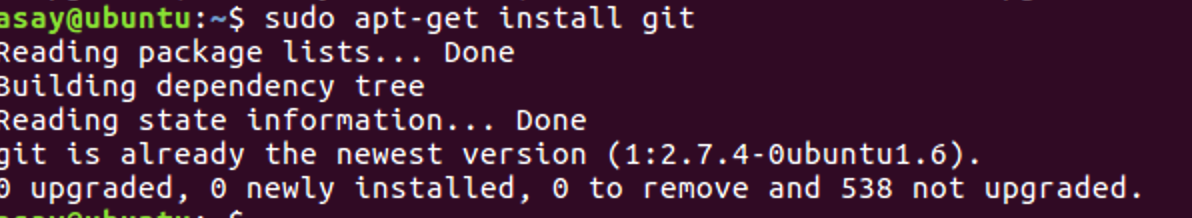
\includegraphics[width=1\textwidth]{git}
						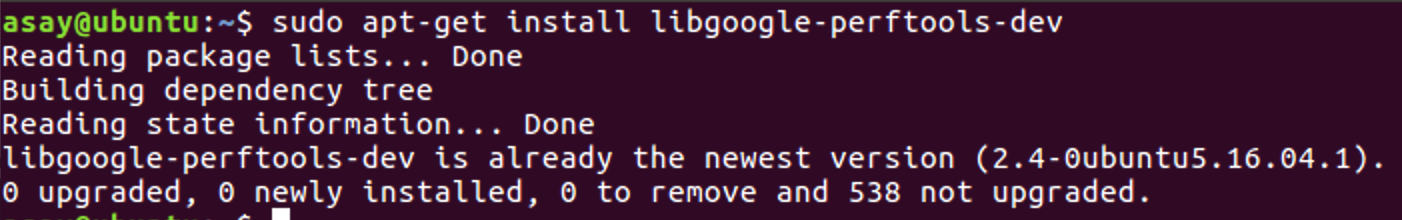
\includegraphics[width=1\textwidth]{libgoogle-proftools}
						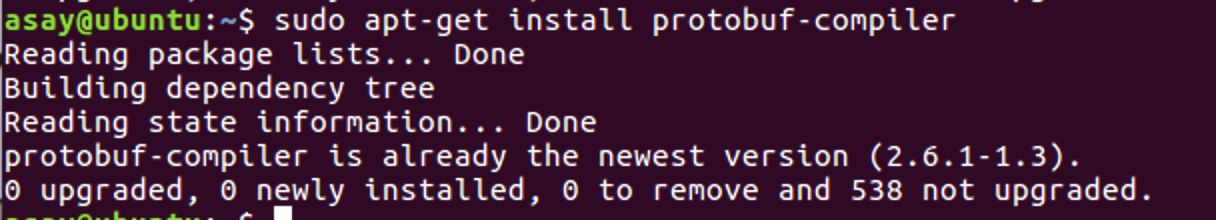
\includegraphics[width=1\textwidth]{libprotobuf-compiler}
							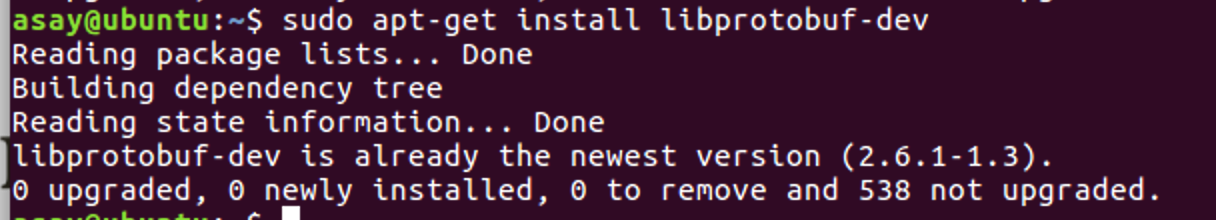
\includegraphics[width=1\textwidth]{libprotobuf-dev}
							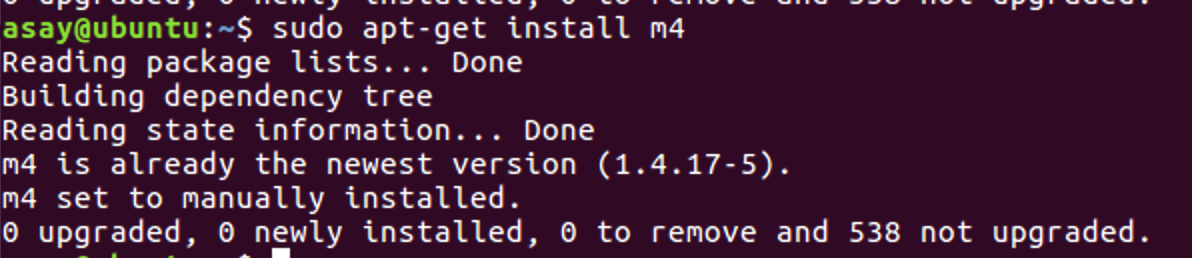
\includegraphics[width=1\textwidth]{m4}
							
\includegraphics[width=1\textwidth]{python}
							
\includegraphics[width=1\textwidth]{python-dev}
							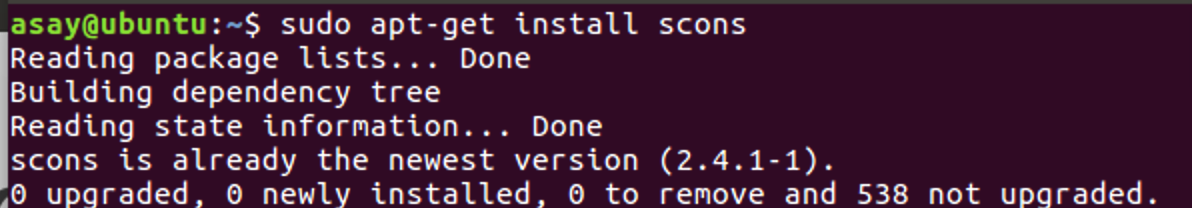
\includegraphics[width=1\textwidth]{scons}
							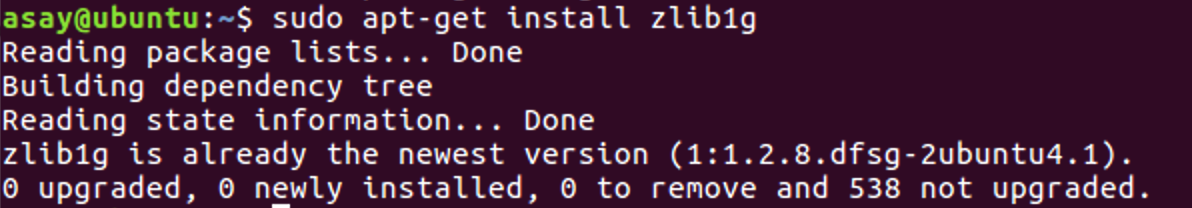
\includegraphics[width=1\textwidth]{zlib1g}
							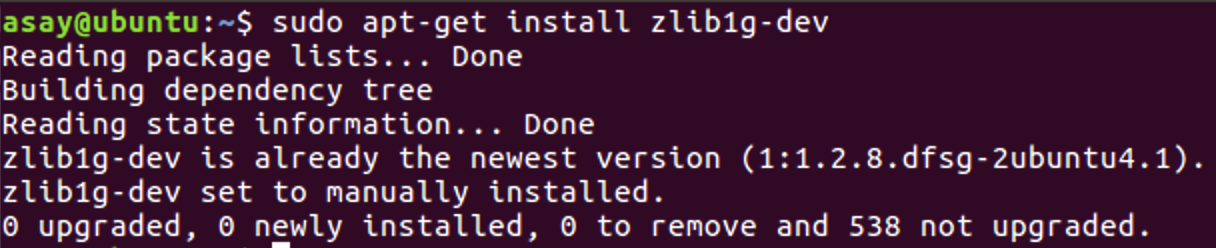
\includegraphics[width=1\textwidth]{zlib1g-dev}
						
					
						
						
	\end{center}



\section*{نصب 
	\lr{gem5}
	با فرض استفاده از معماری 
	\lr{x86} }
\subsection*{\textcolor{red}{\lr{GIT CLONE}}}
\begin{center}
								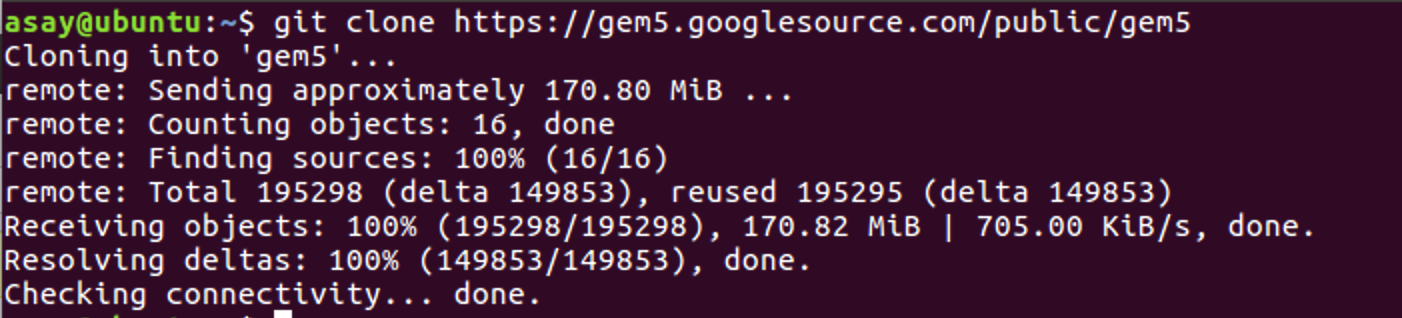
\includegraphics[width=1\textwidth]{gem5-clone}
\end{center}
\subsection*{\textcolor{red}{\lr{BUILD}}}

\begin{center}
	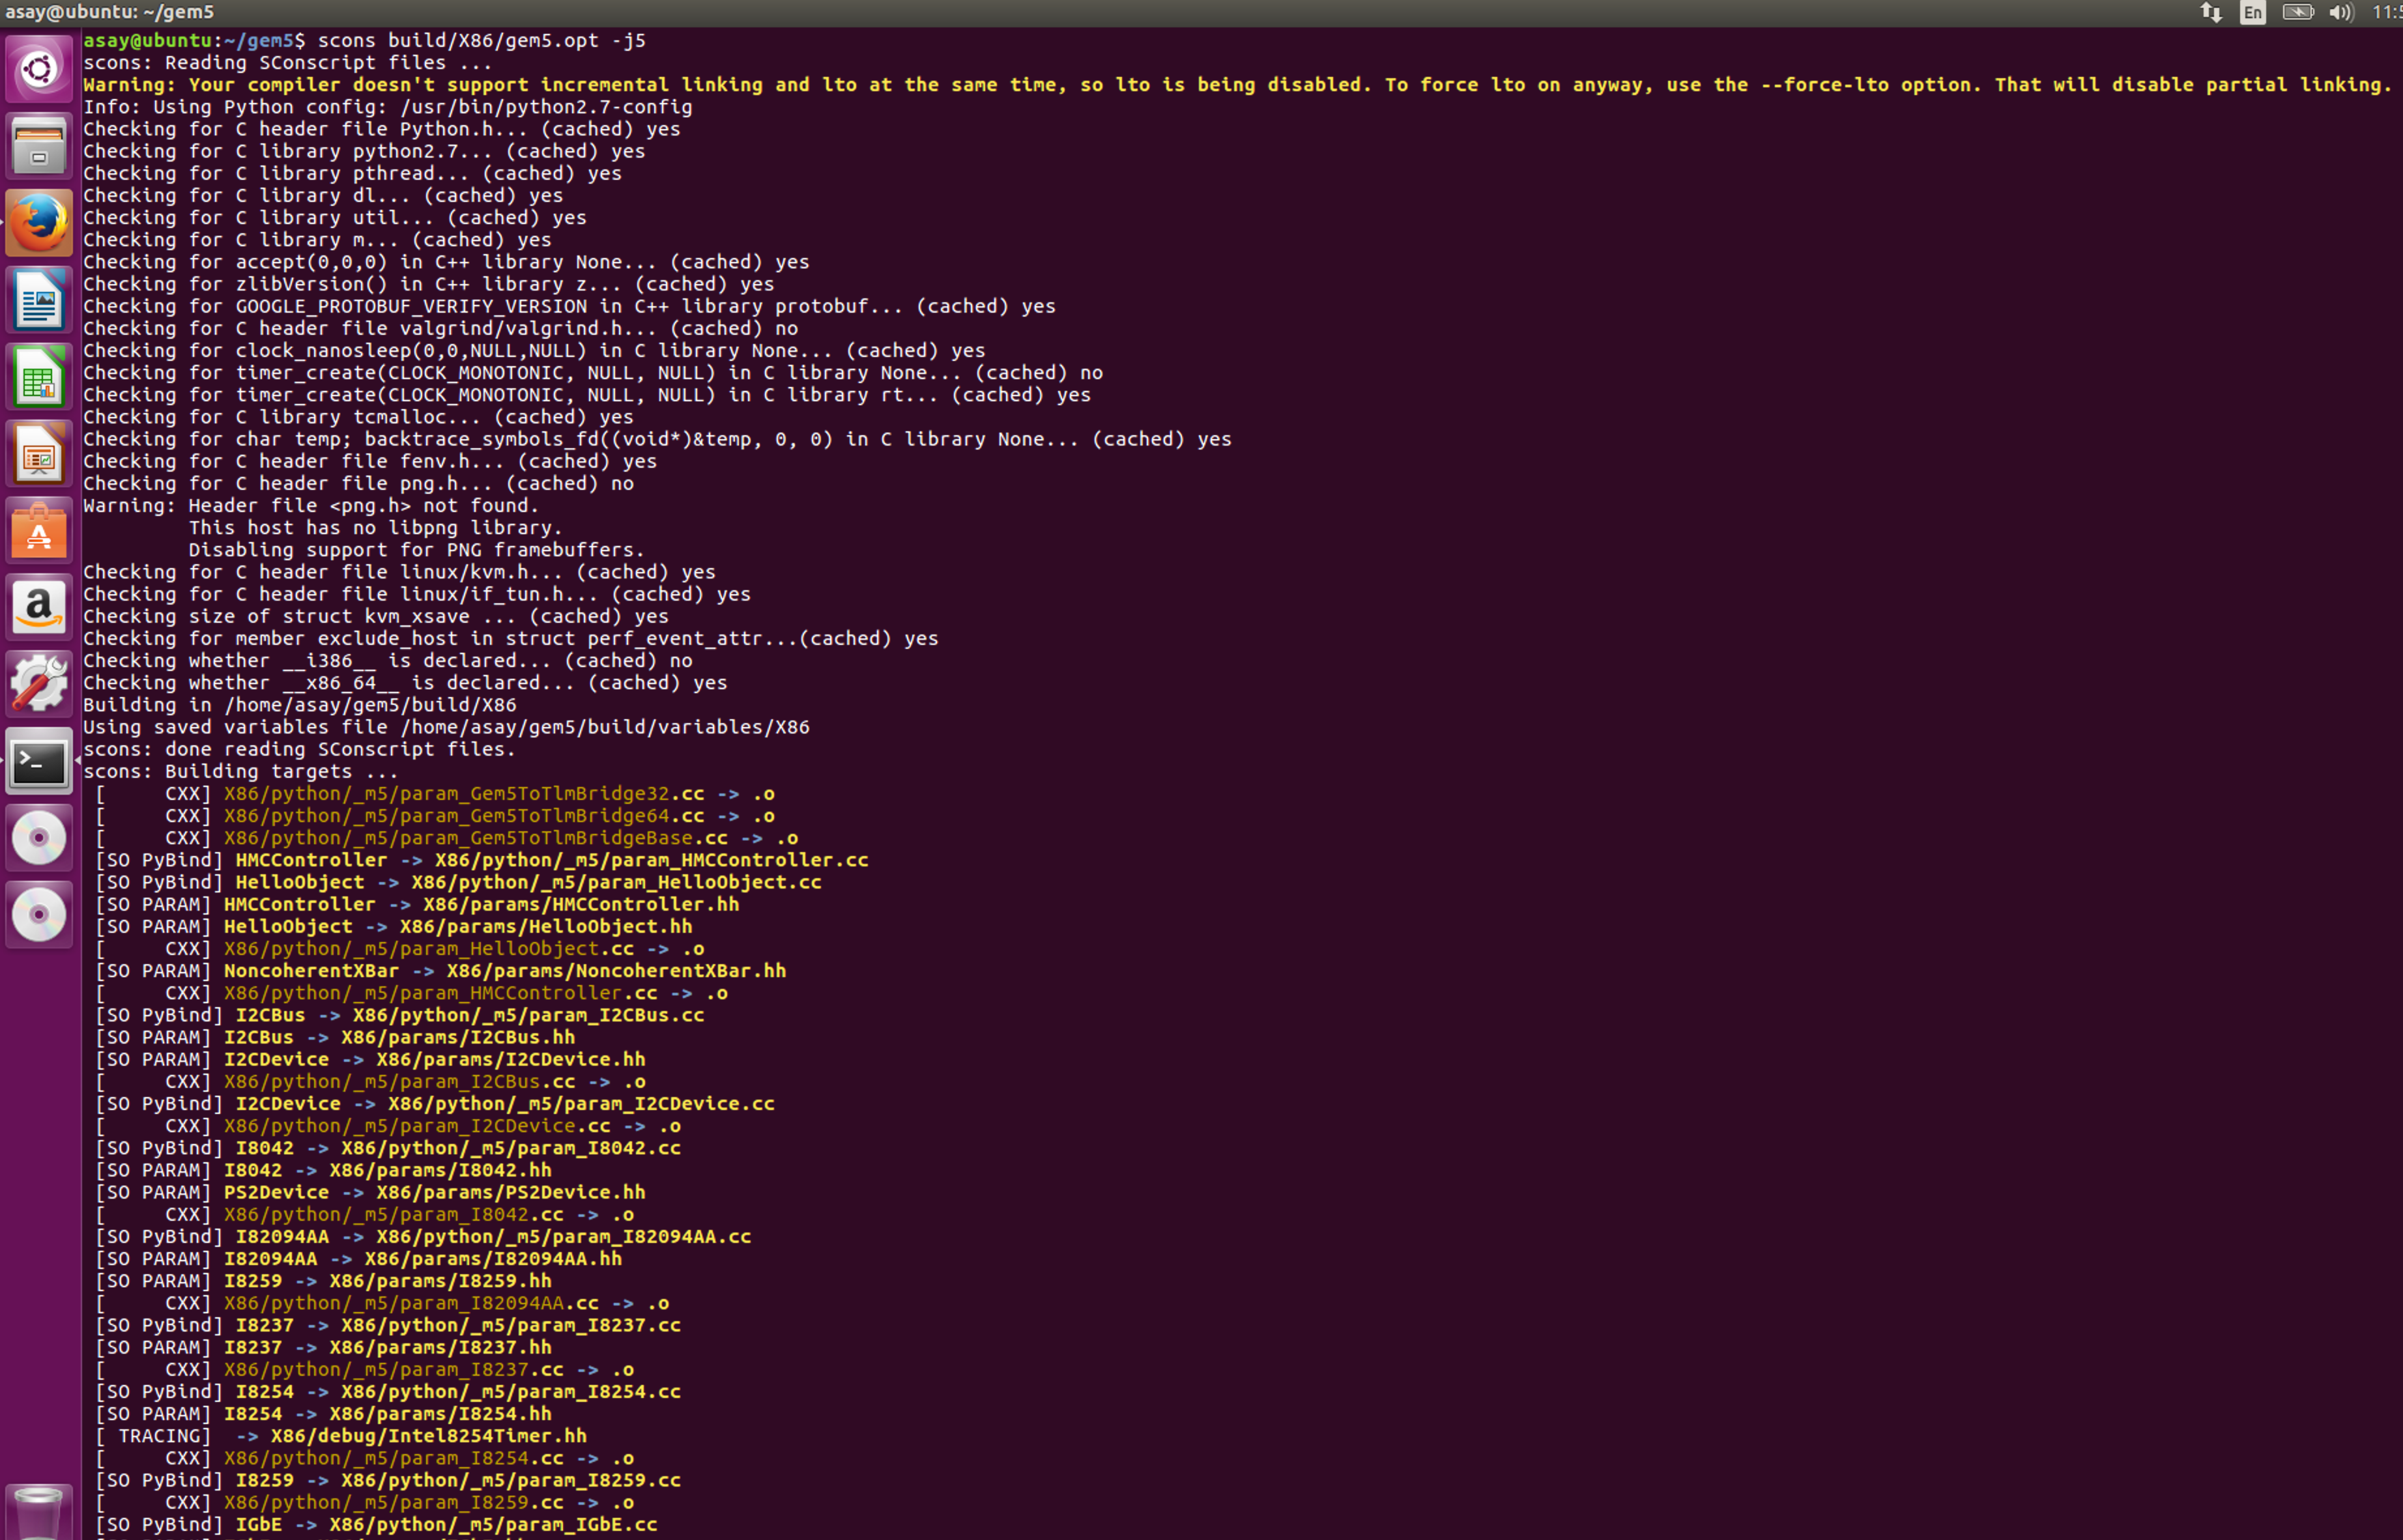
\includegraphics[width=1\textwidth]{build27}
	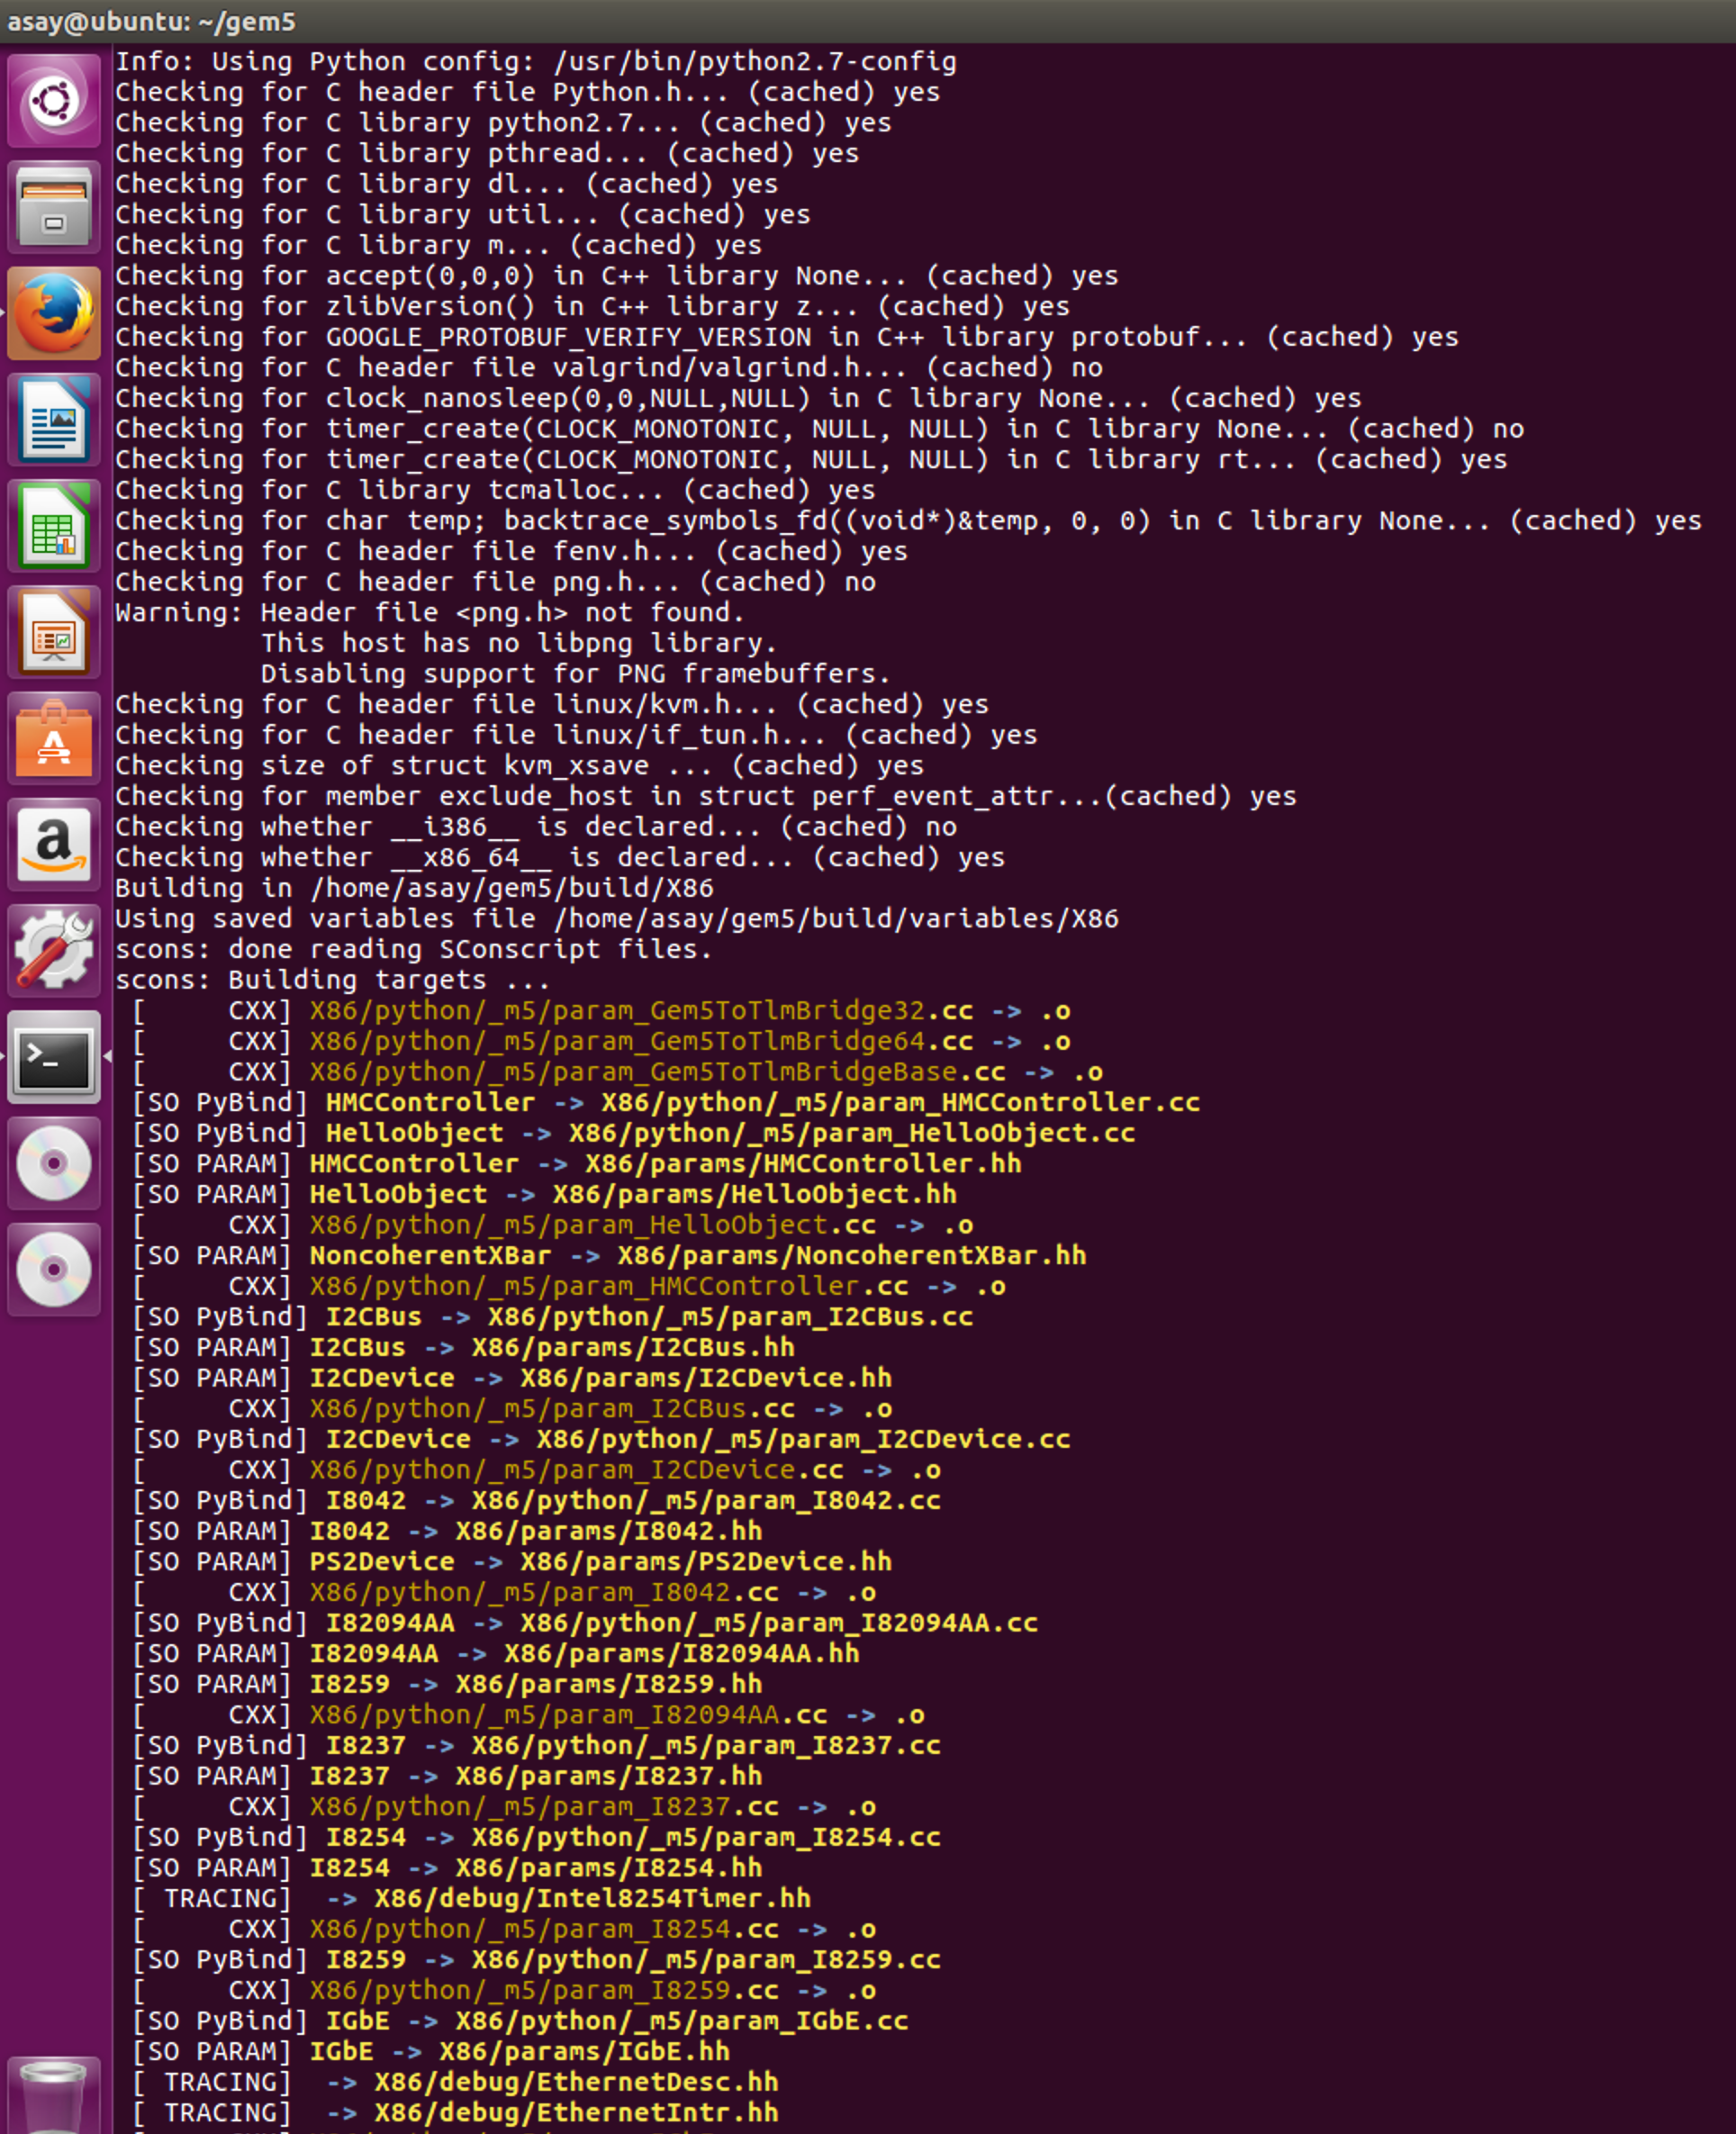
\includegraphics[width=1\textwidth]{build26}
	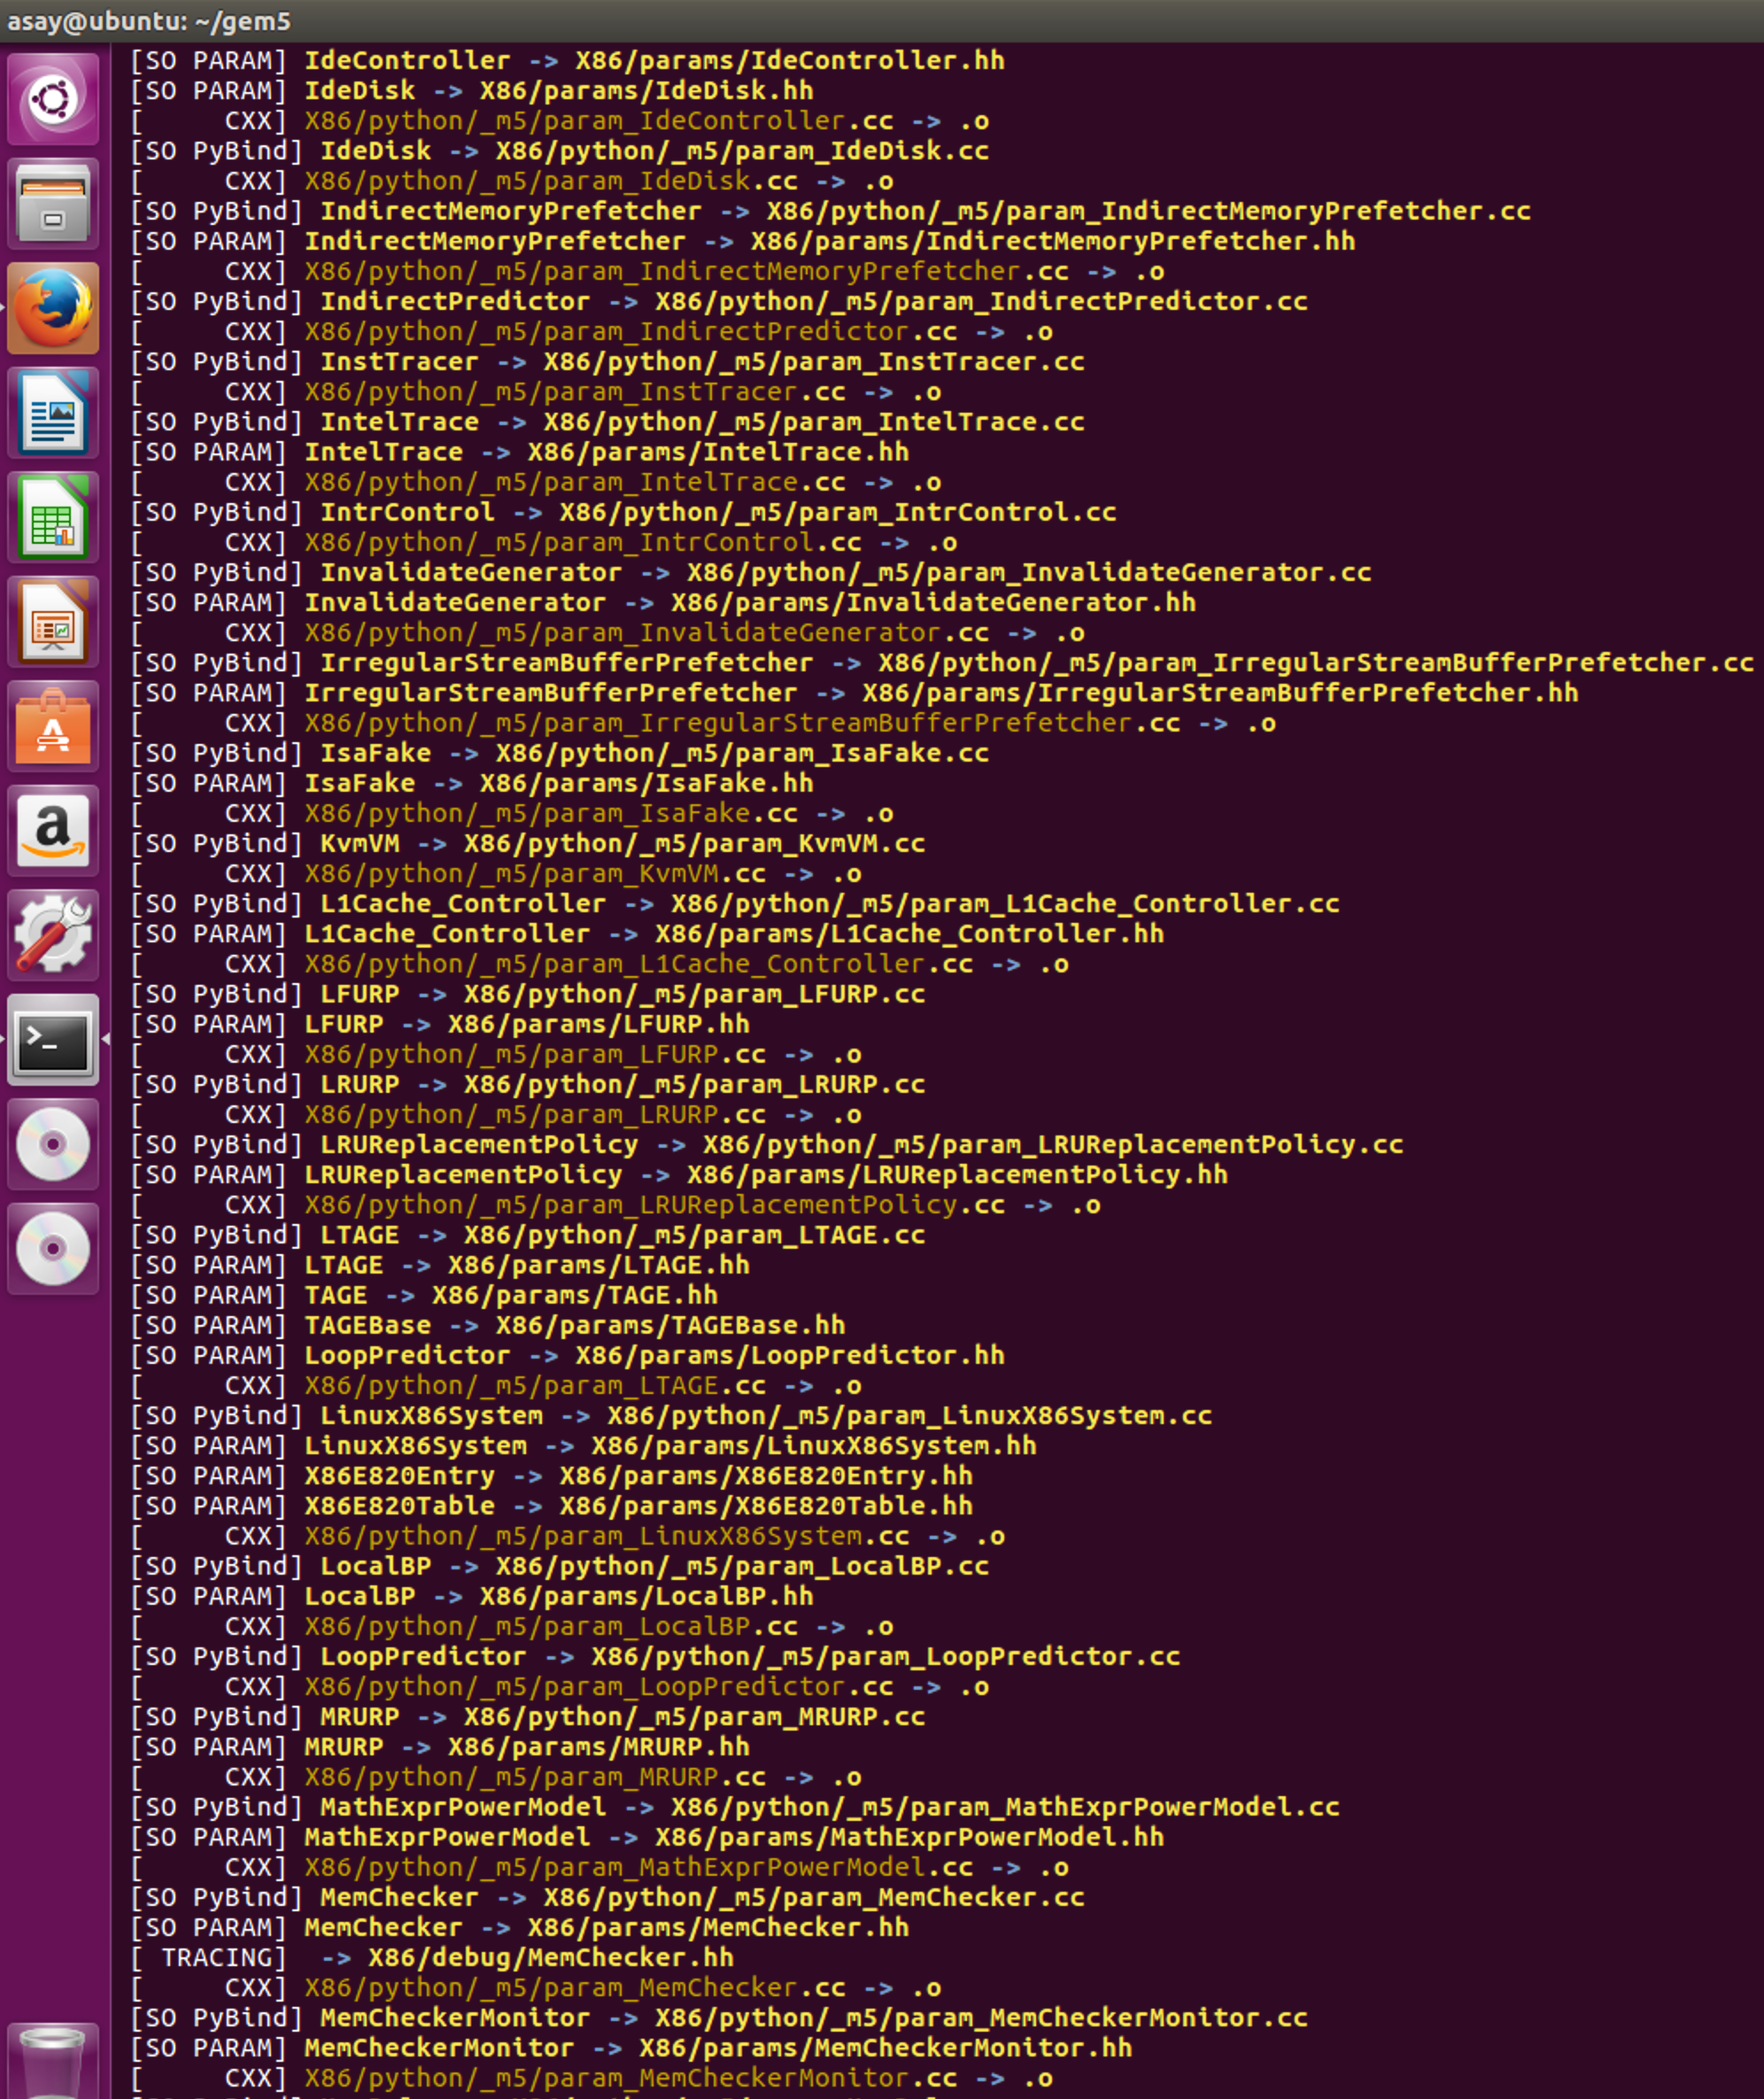
\includegraphics[width=1\textwidth]{build25}
%	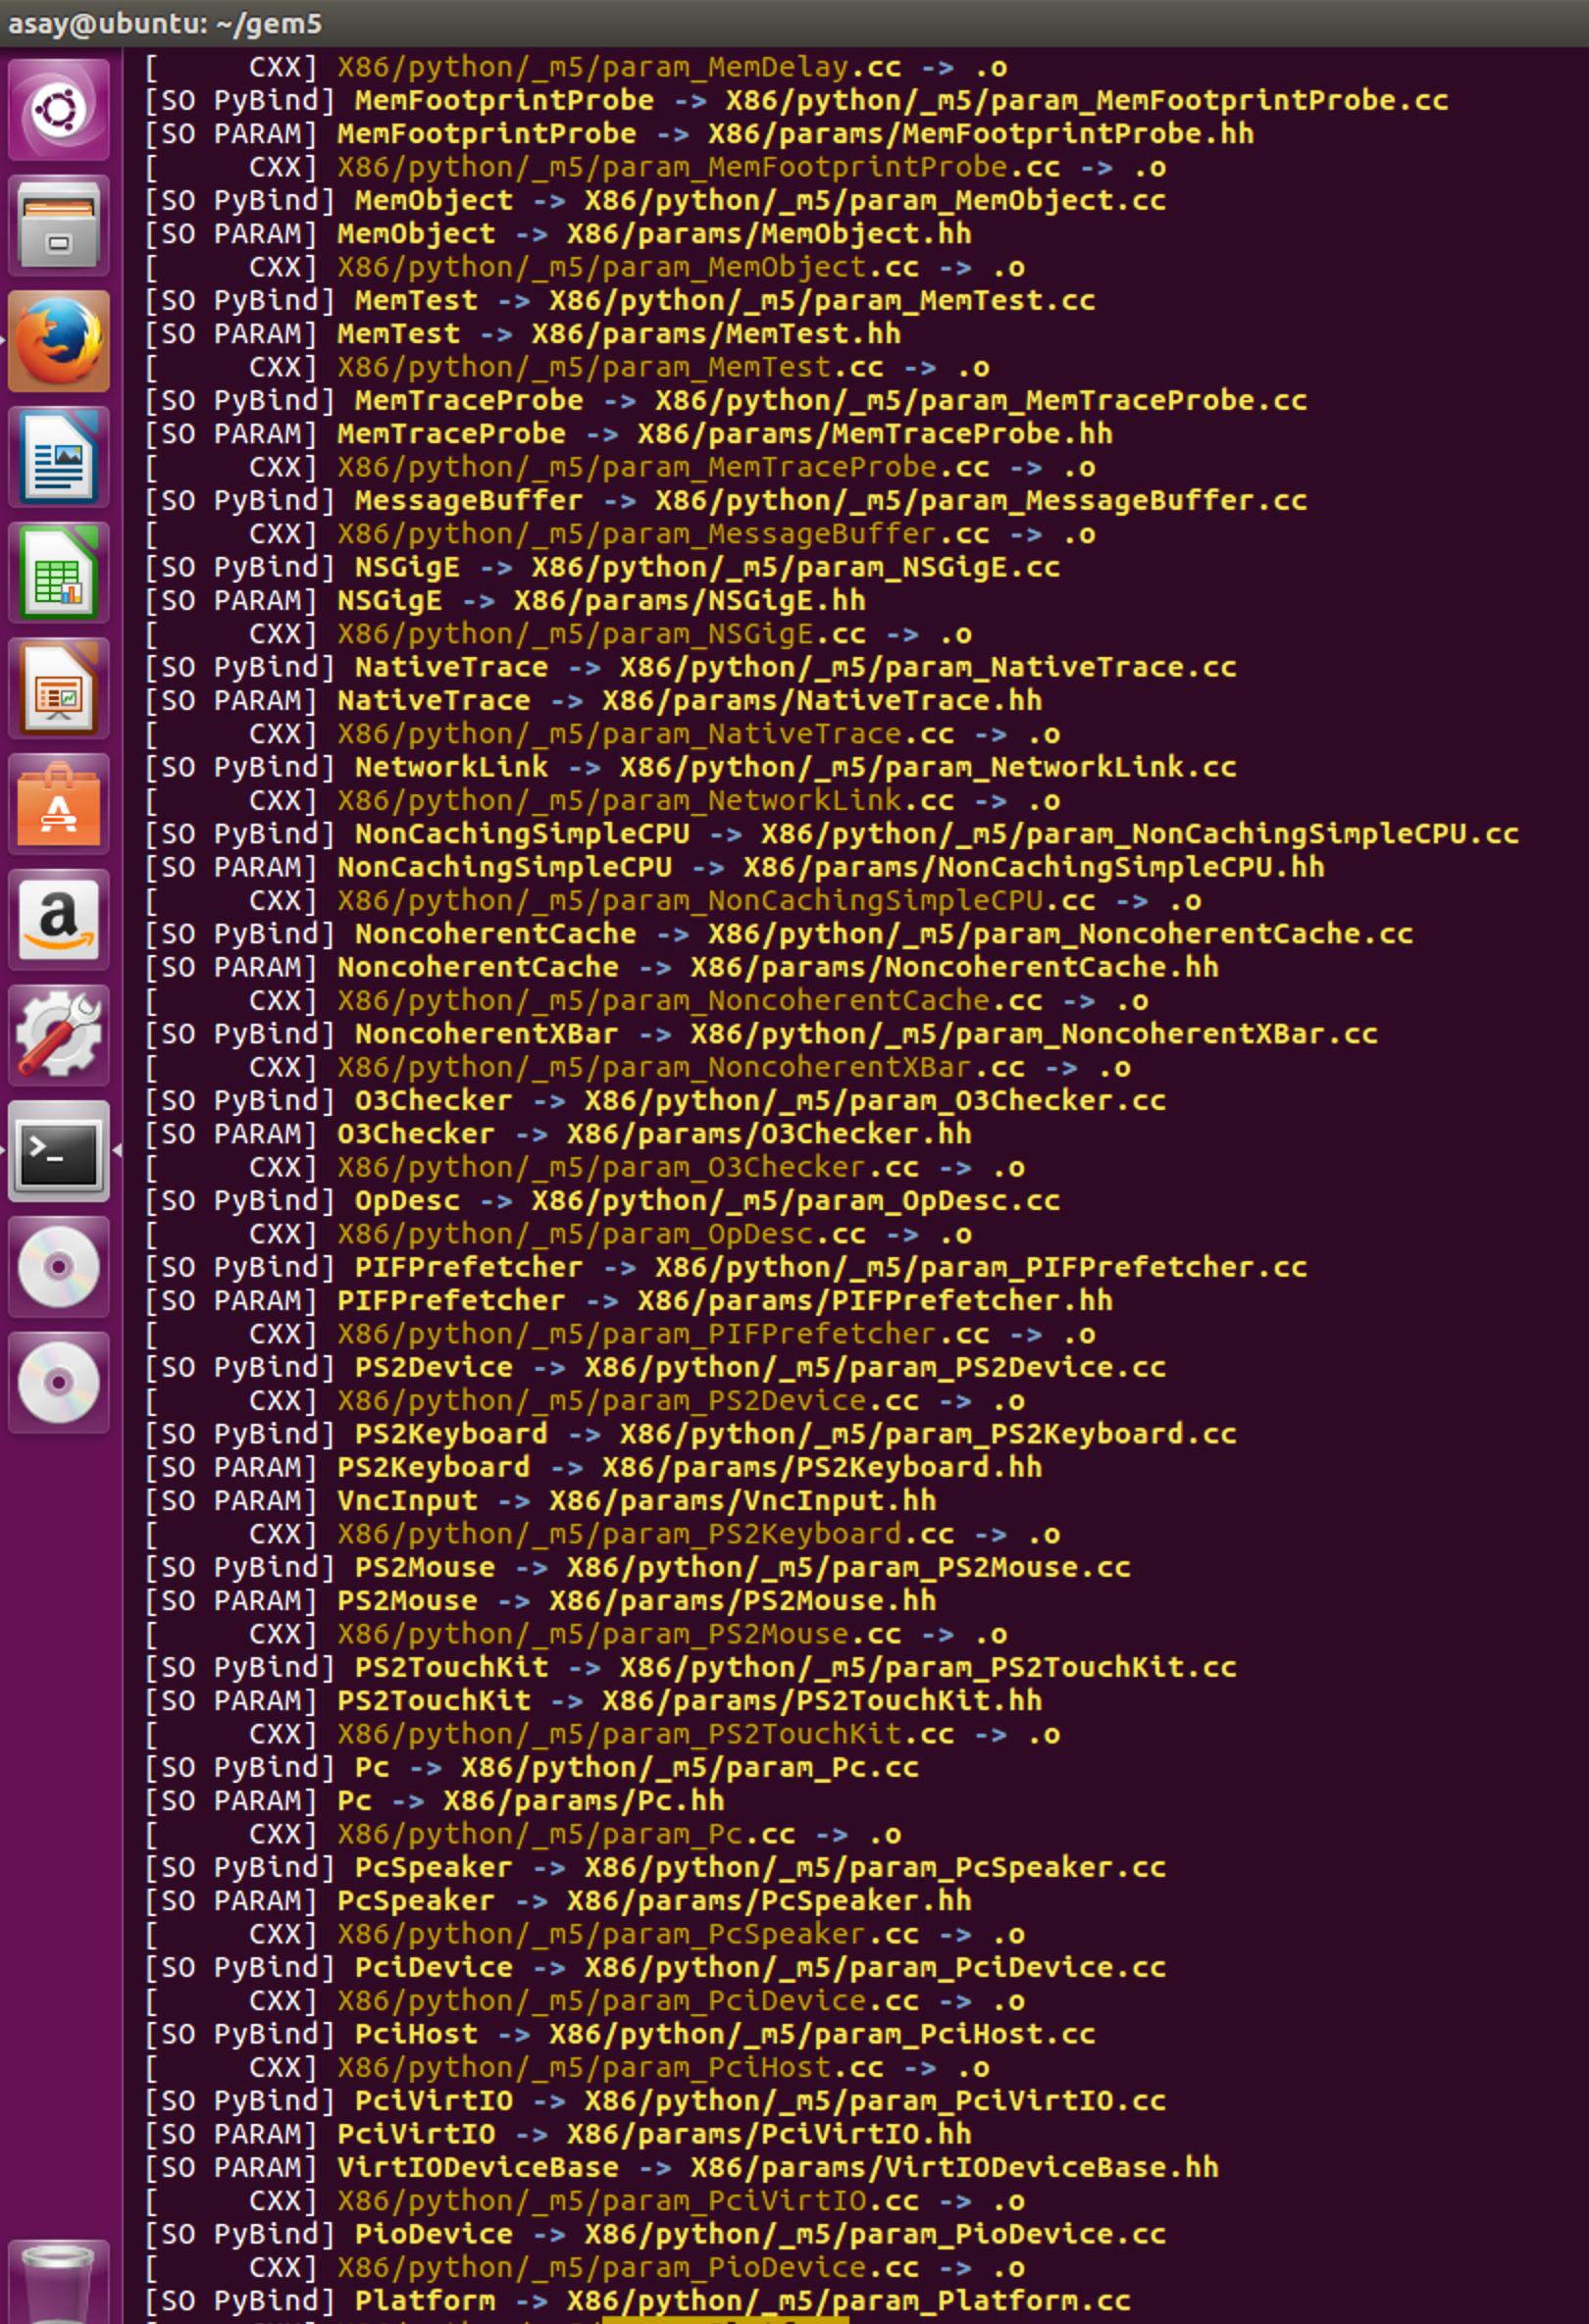
\includegraphics[width=1\textwidth]{build24}
%	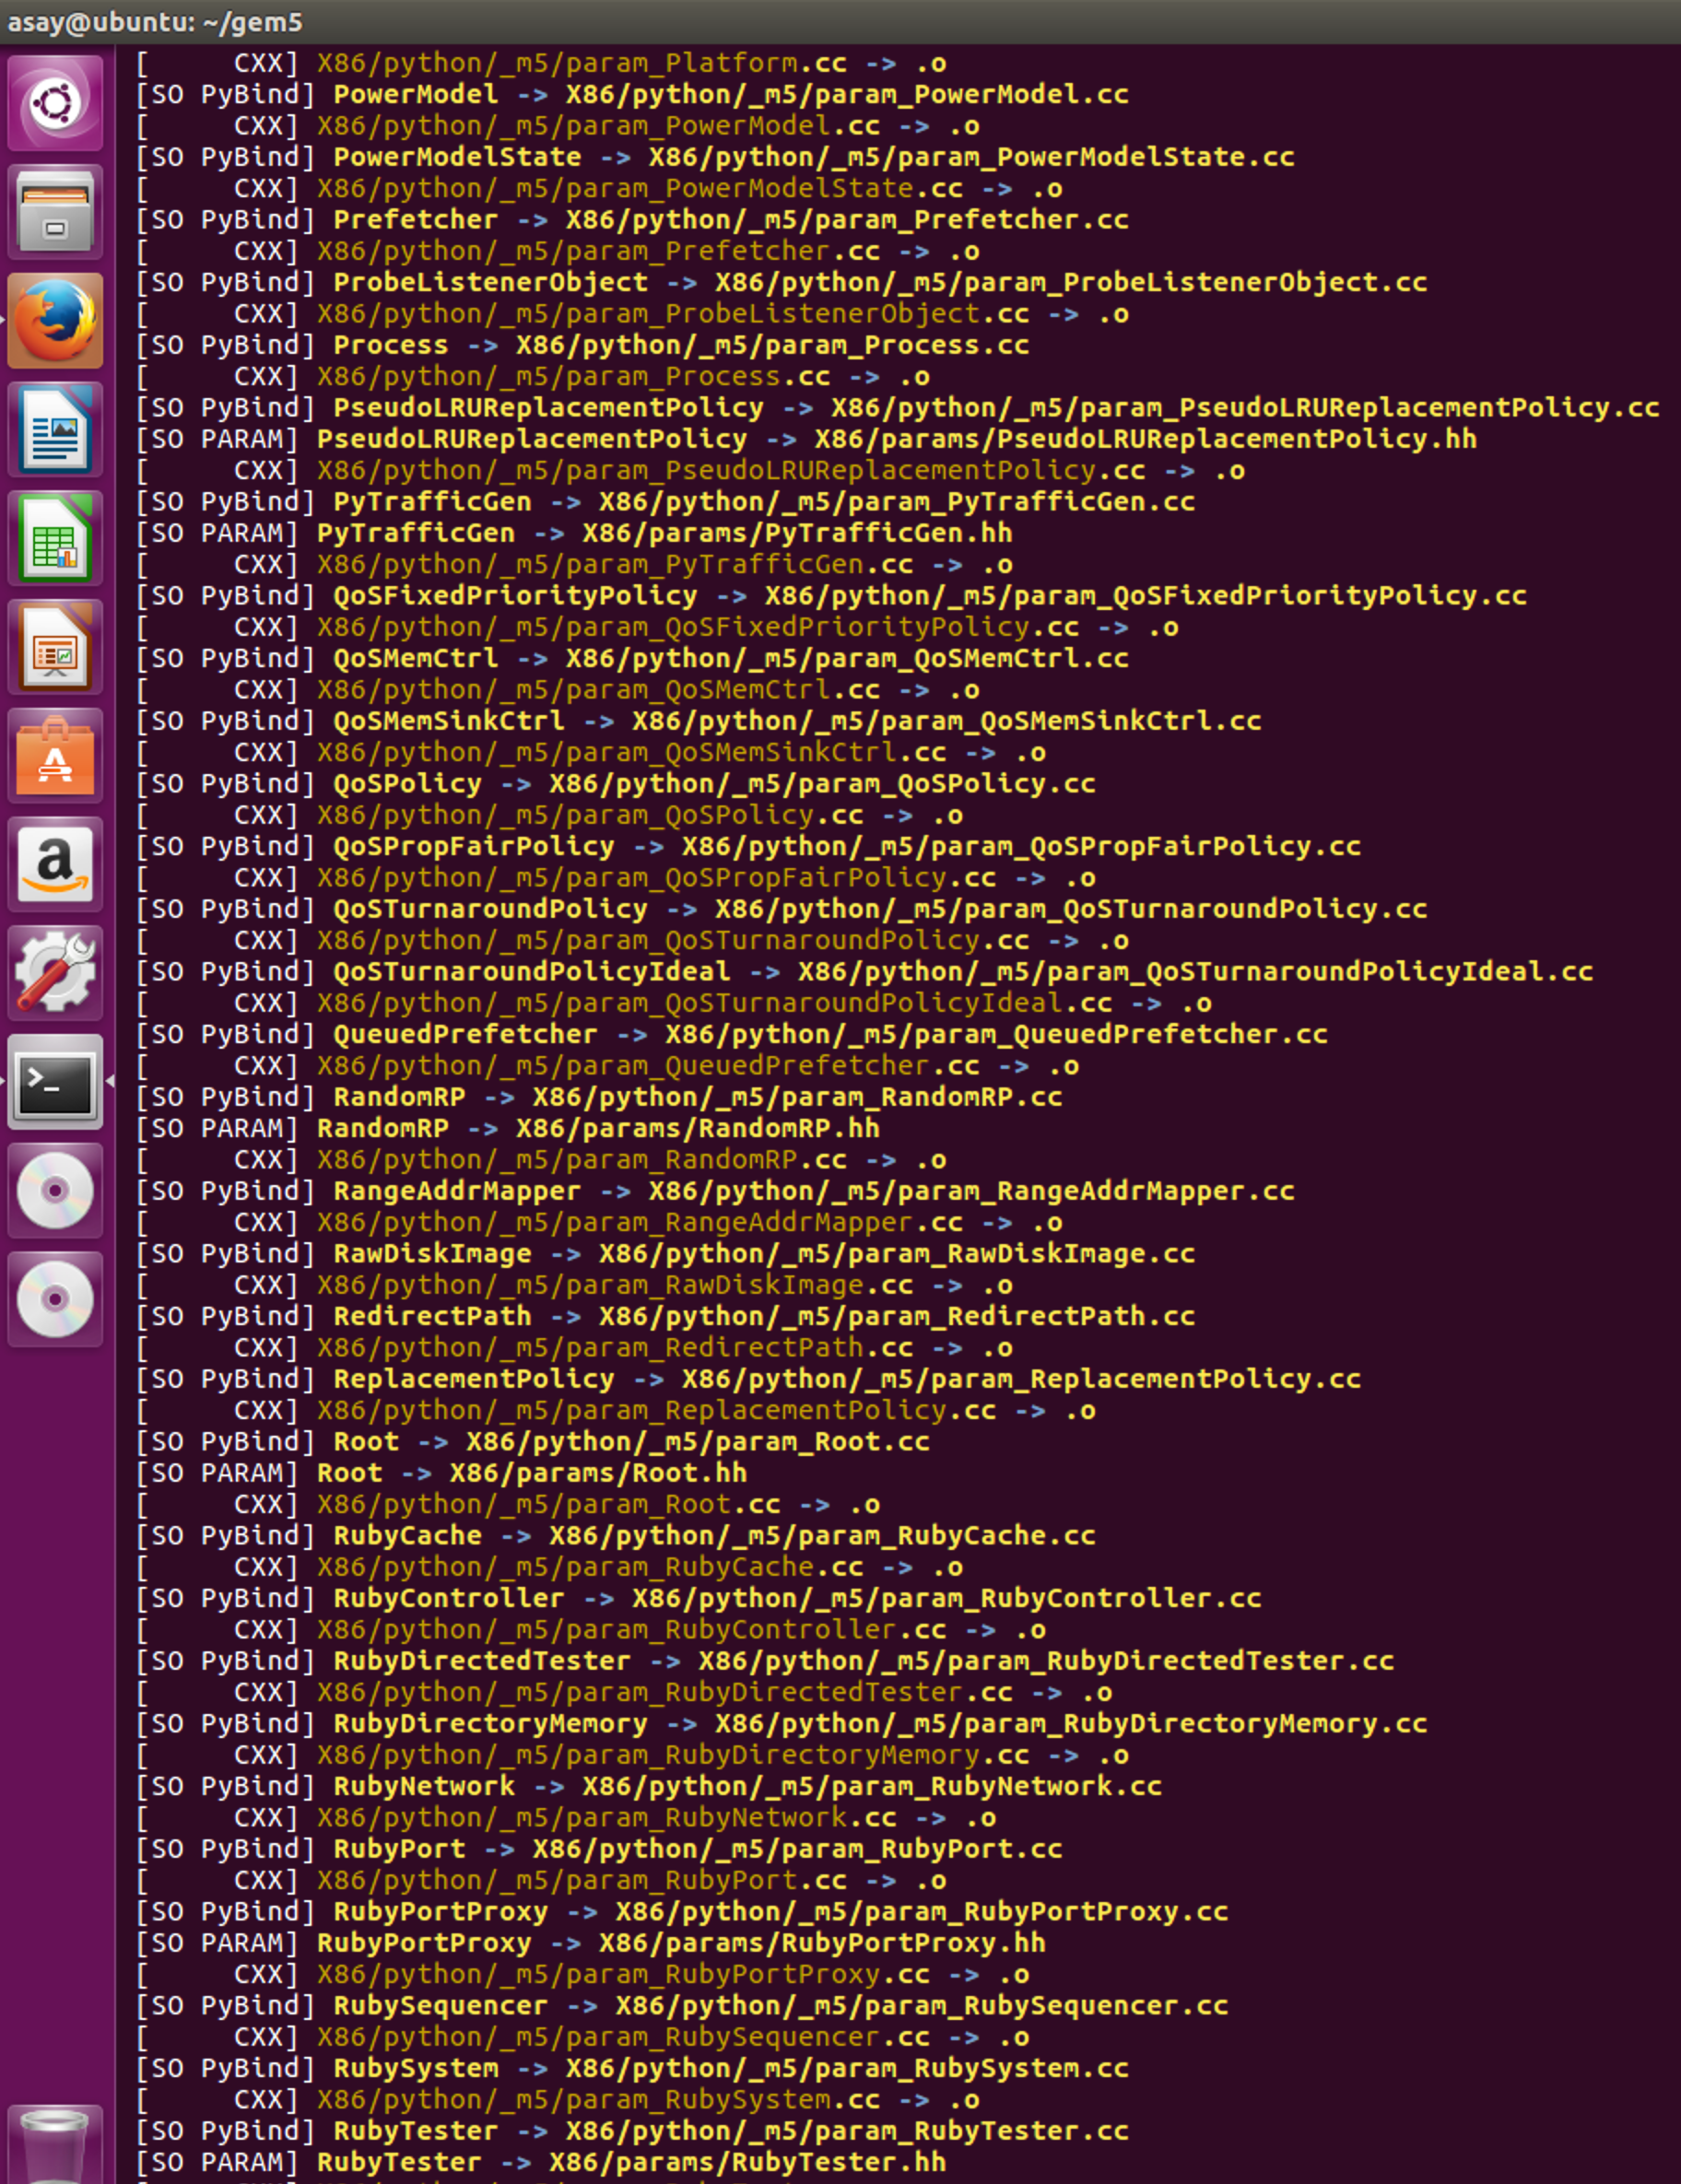
\includegraphics[width=1\textwidth]{build23}
%	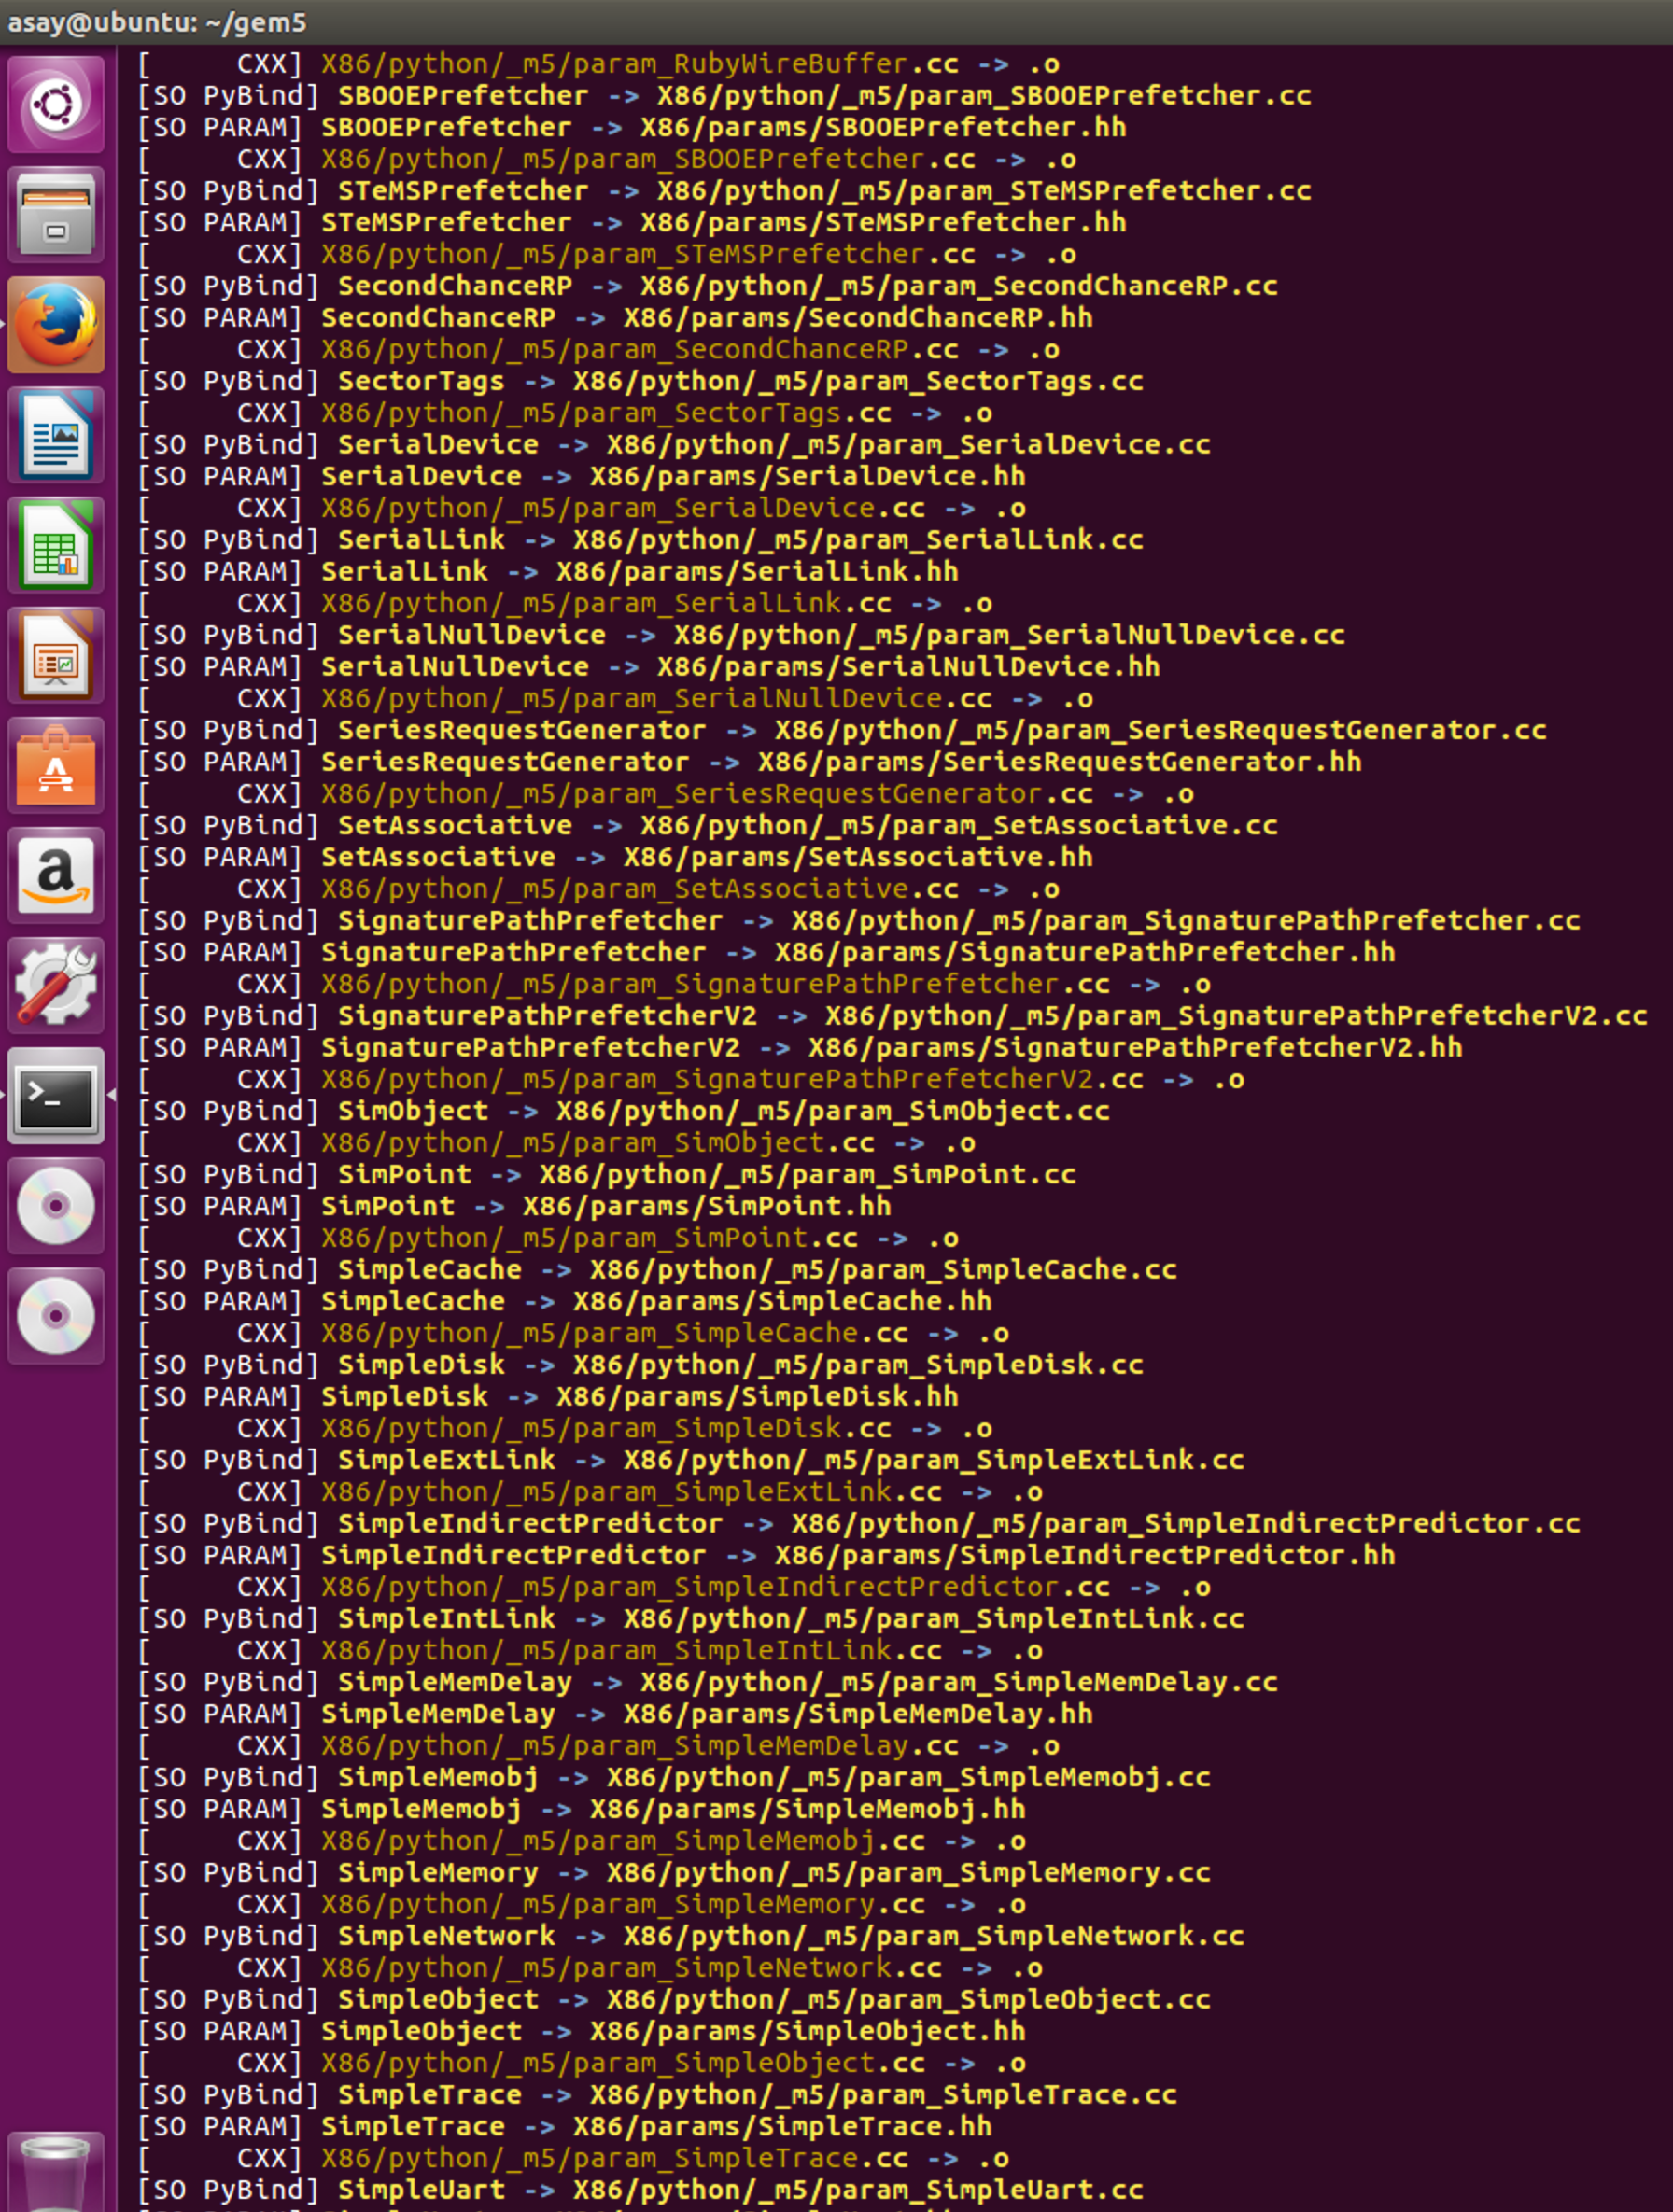
\includegraphics[width=1\textwidth]{build22}
%	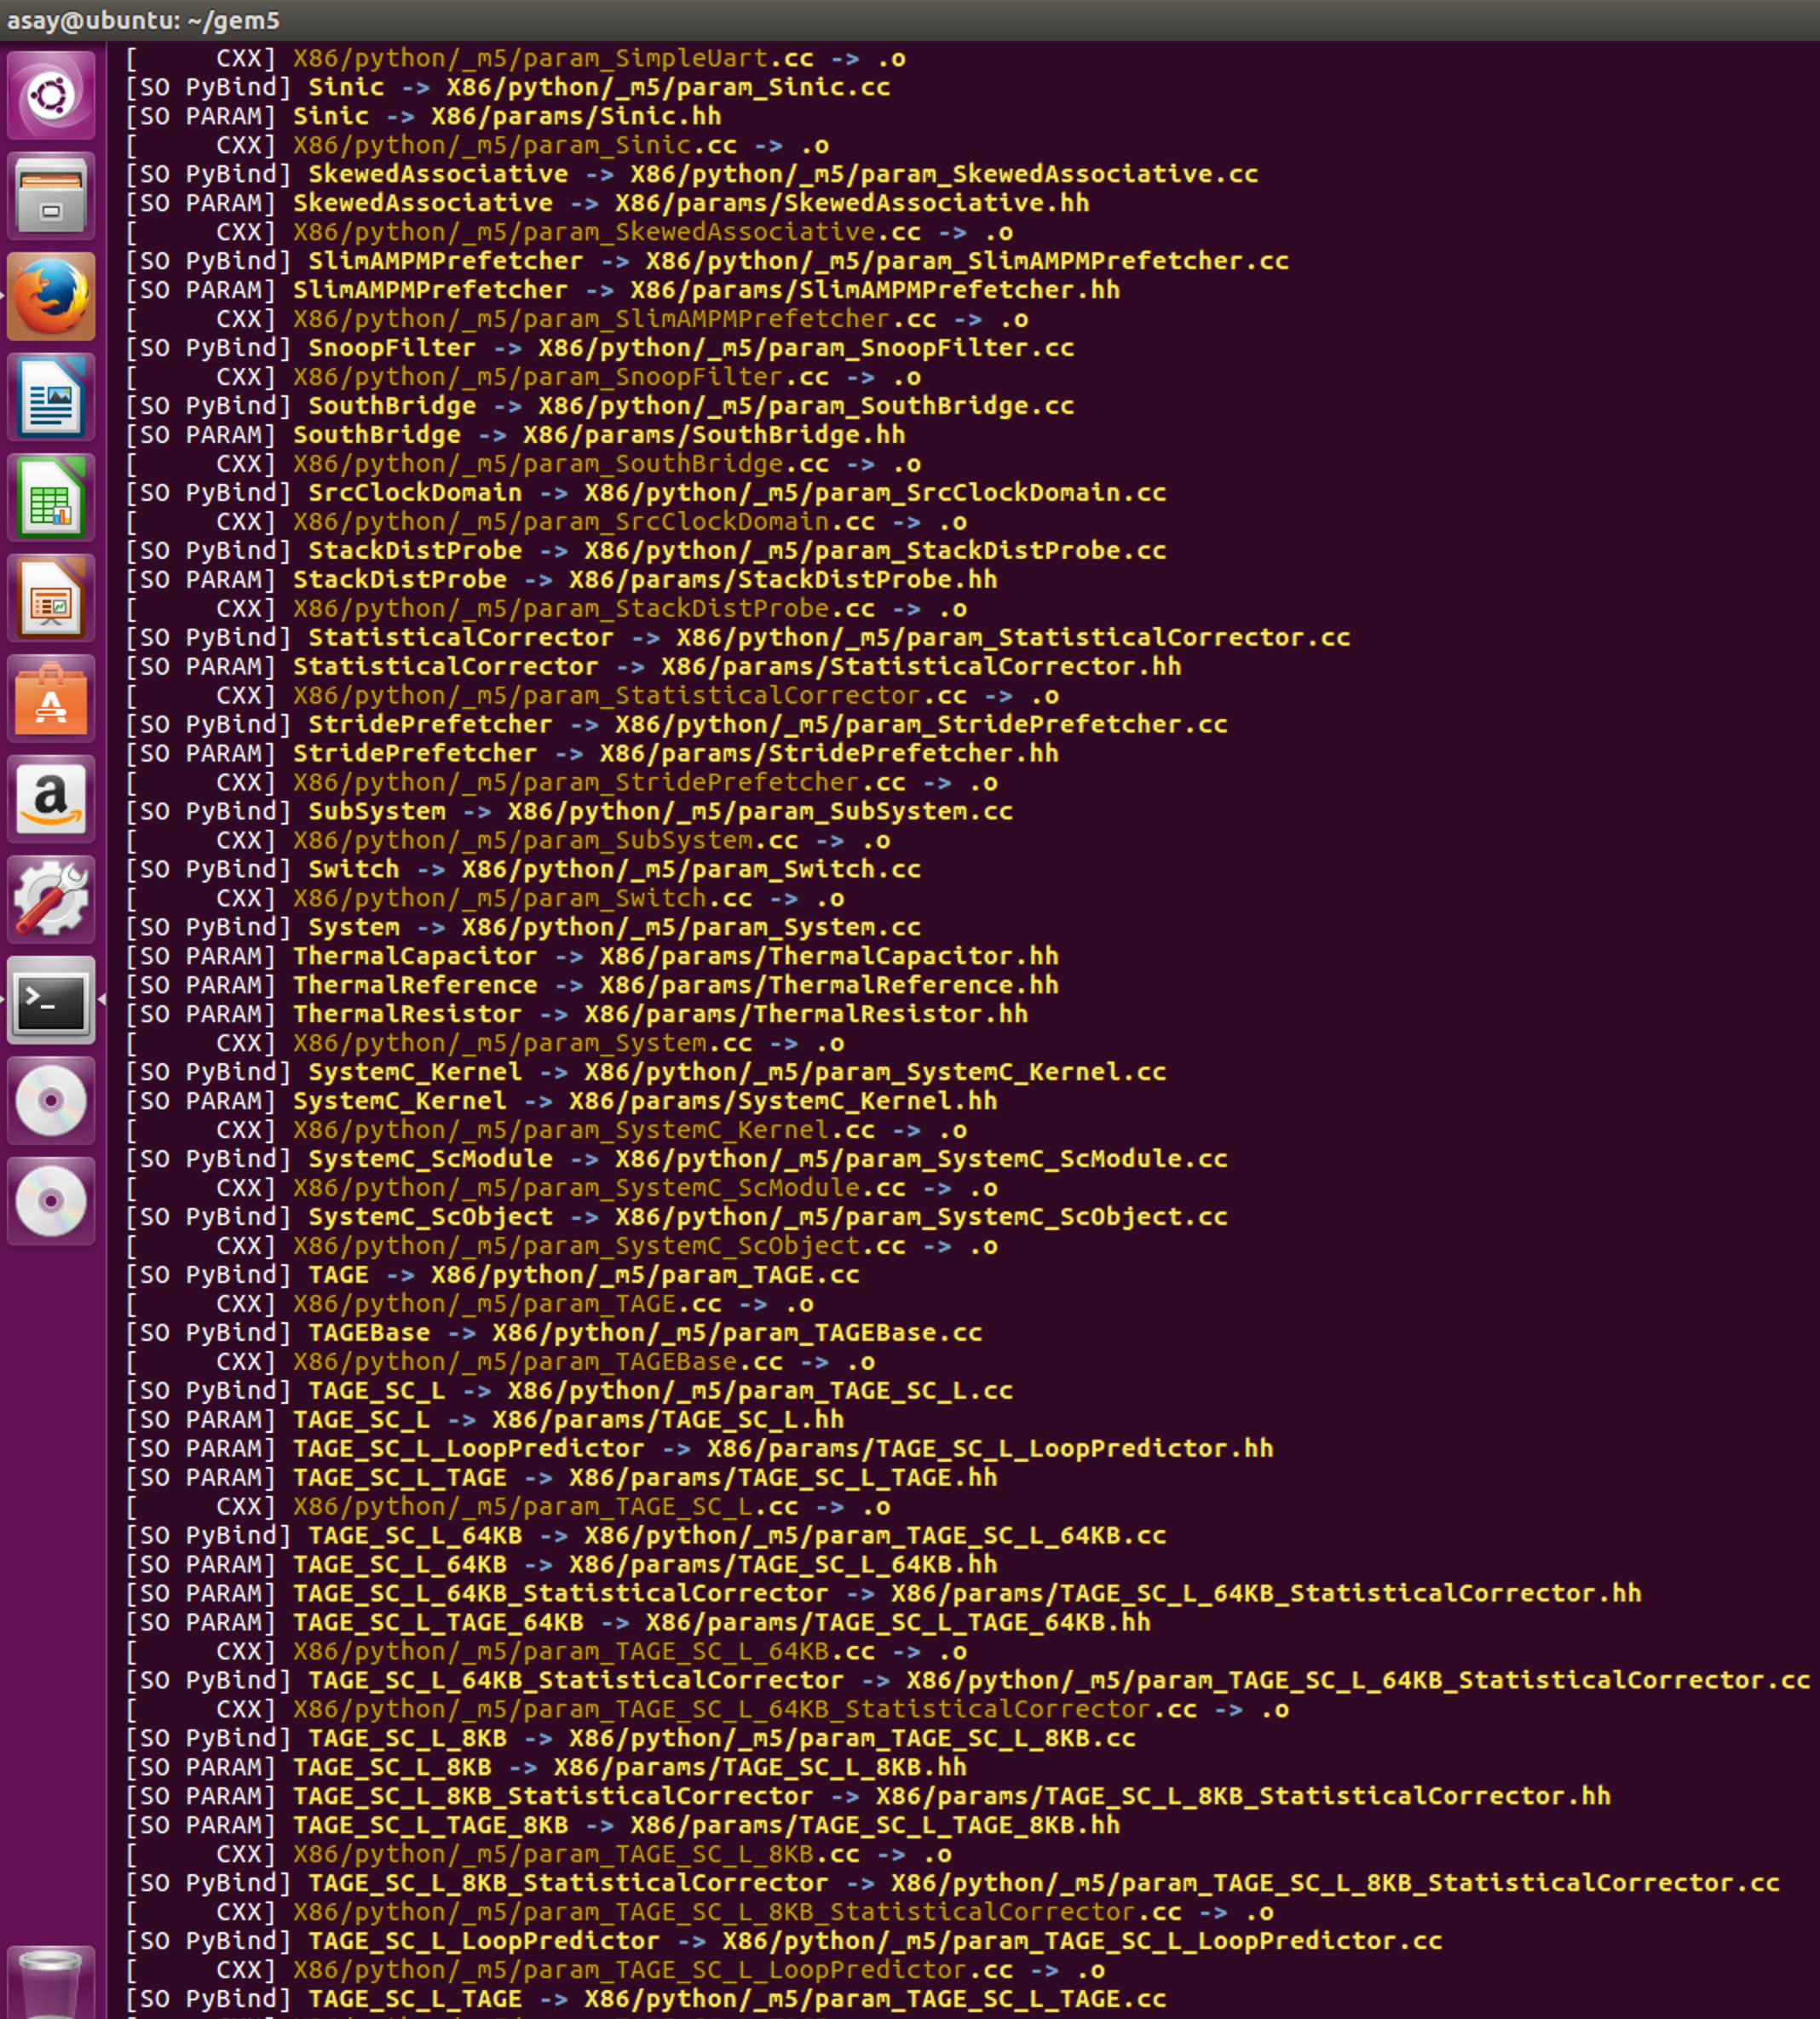
\includegraphics[width=1\textwidth]{build21}
%	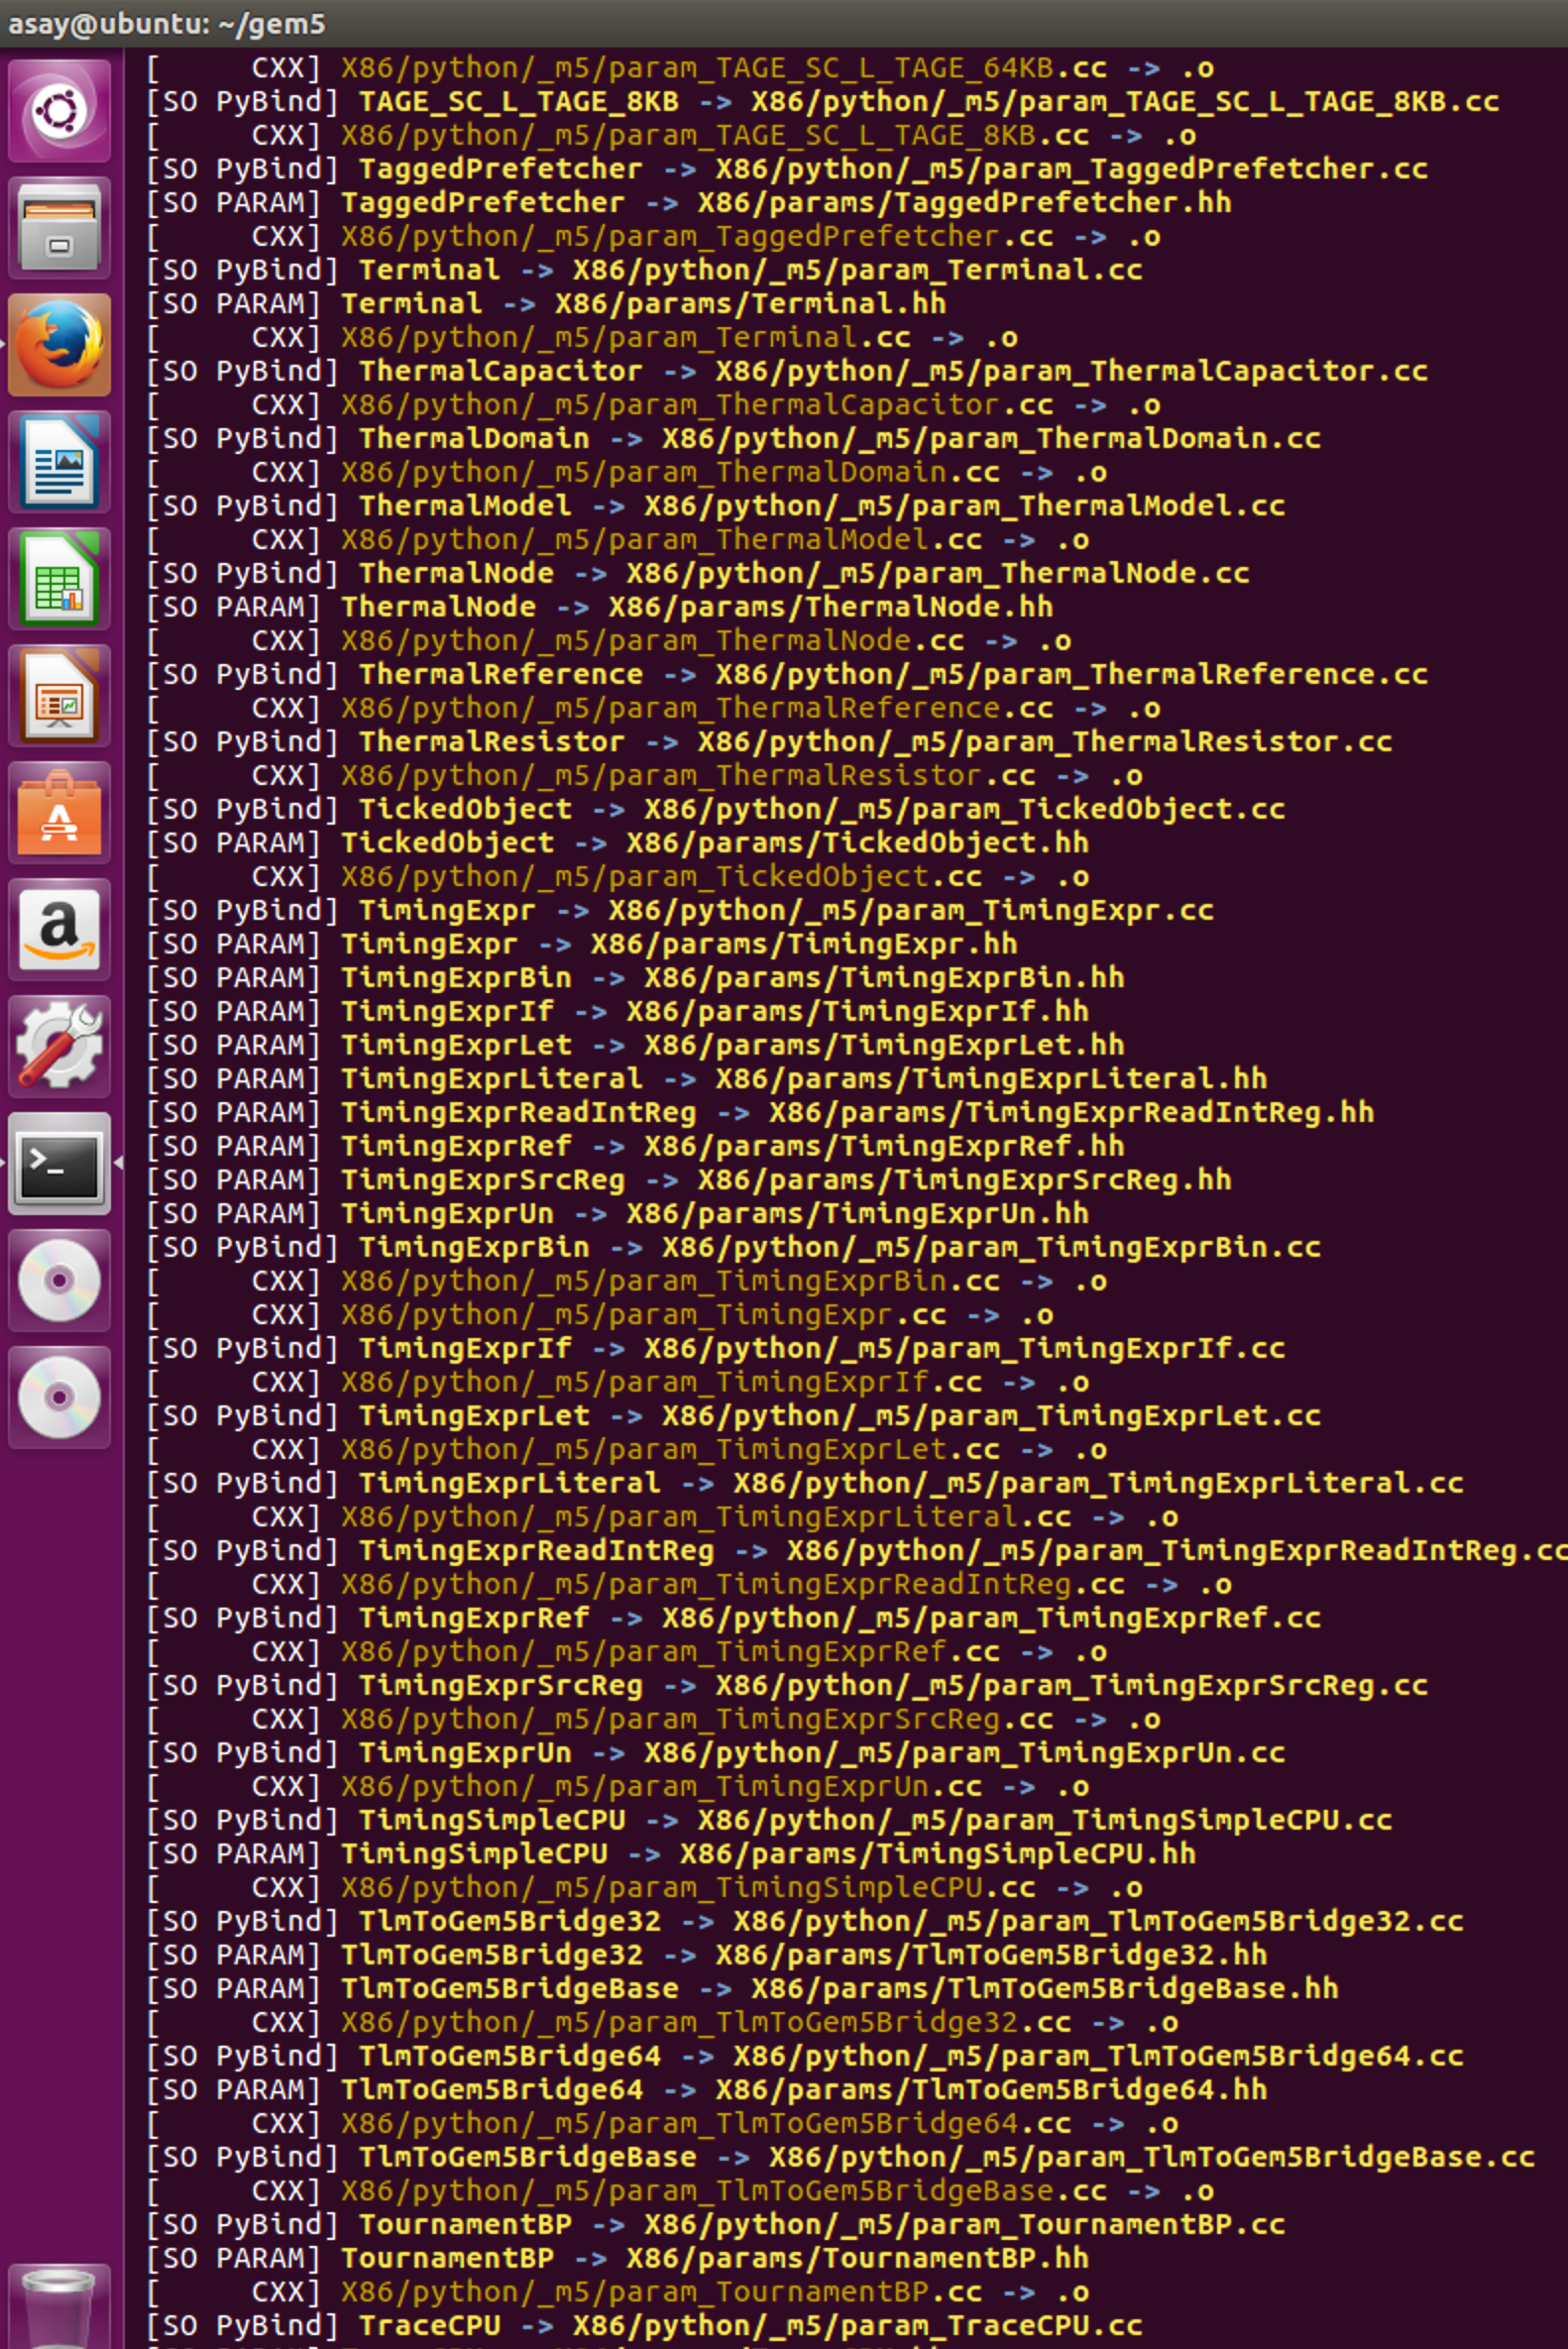
\includegraphics[width=1\textwidth]{build20}
%	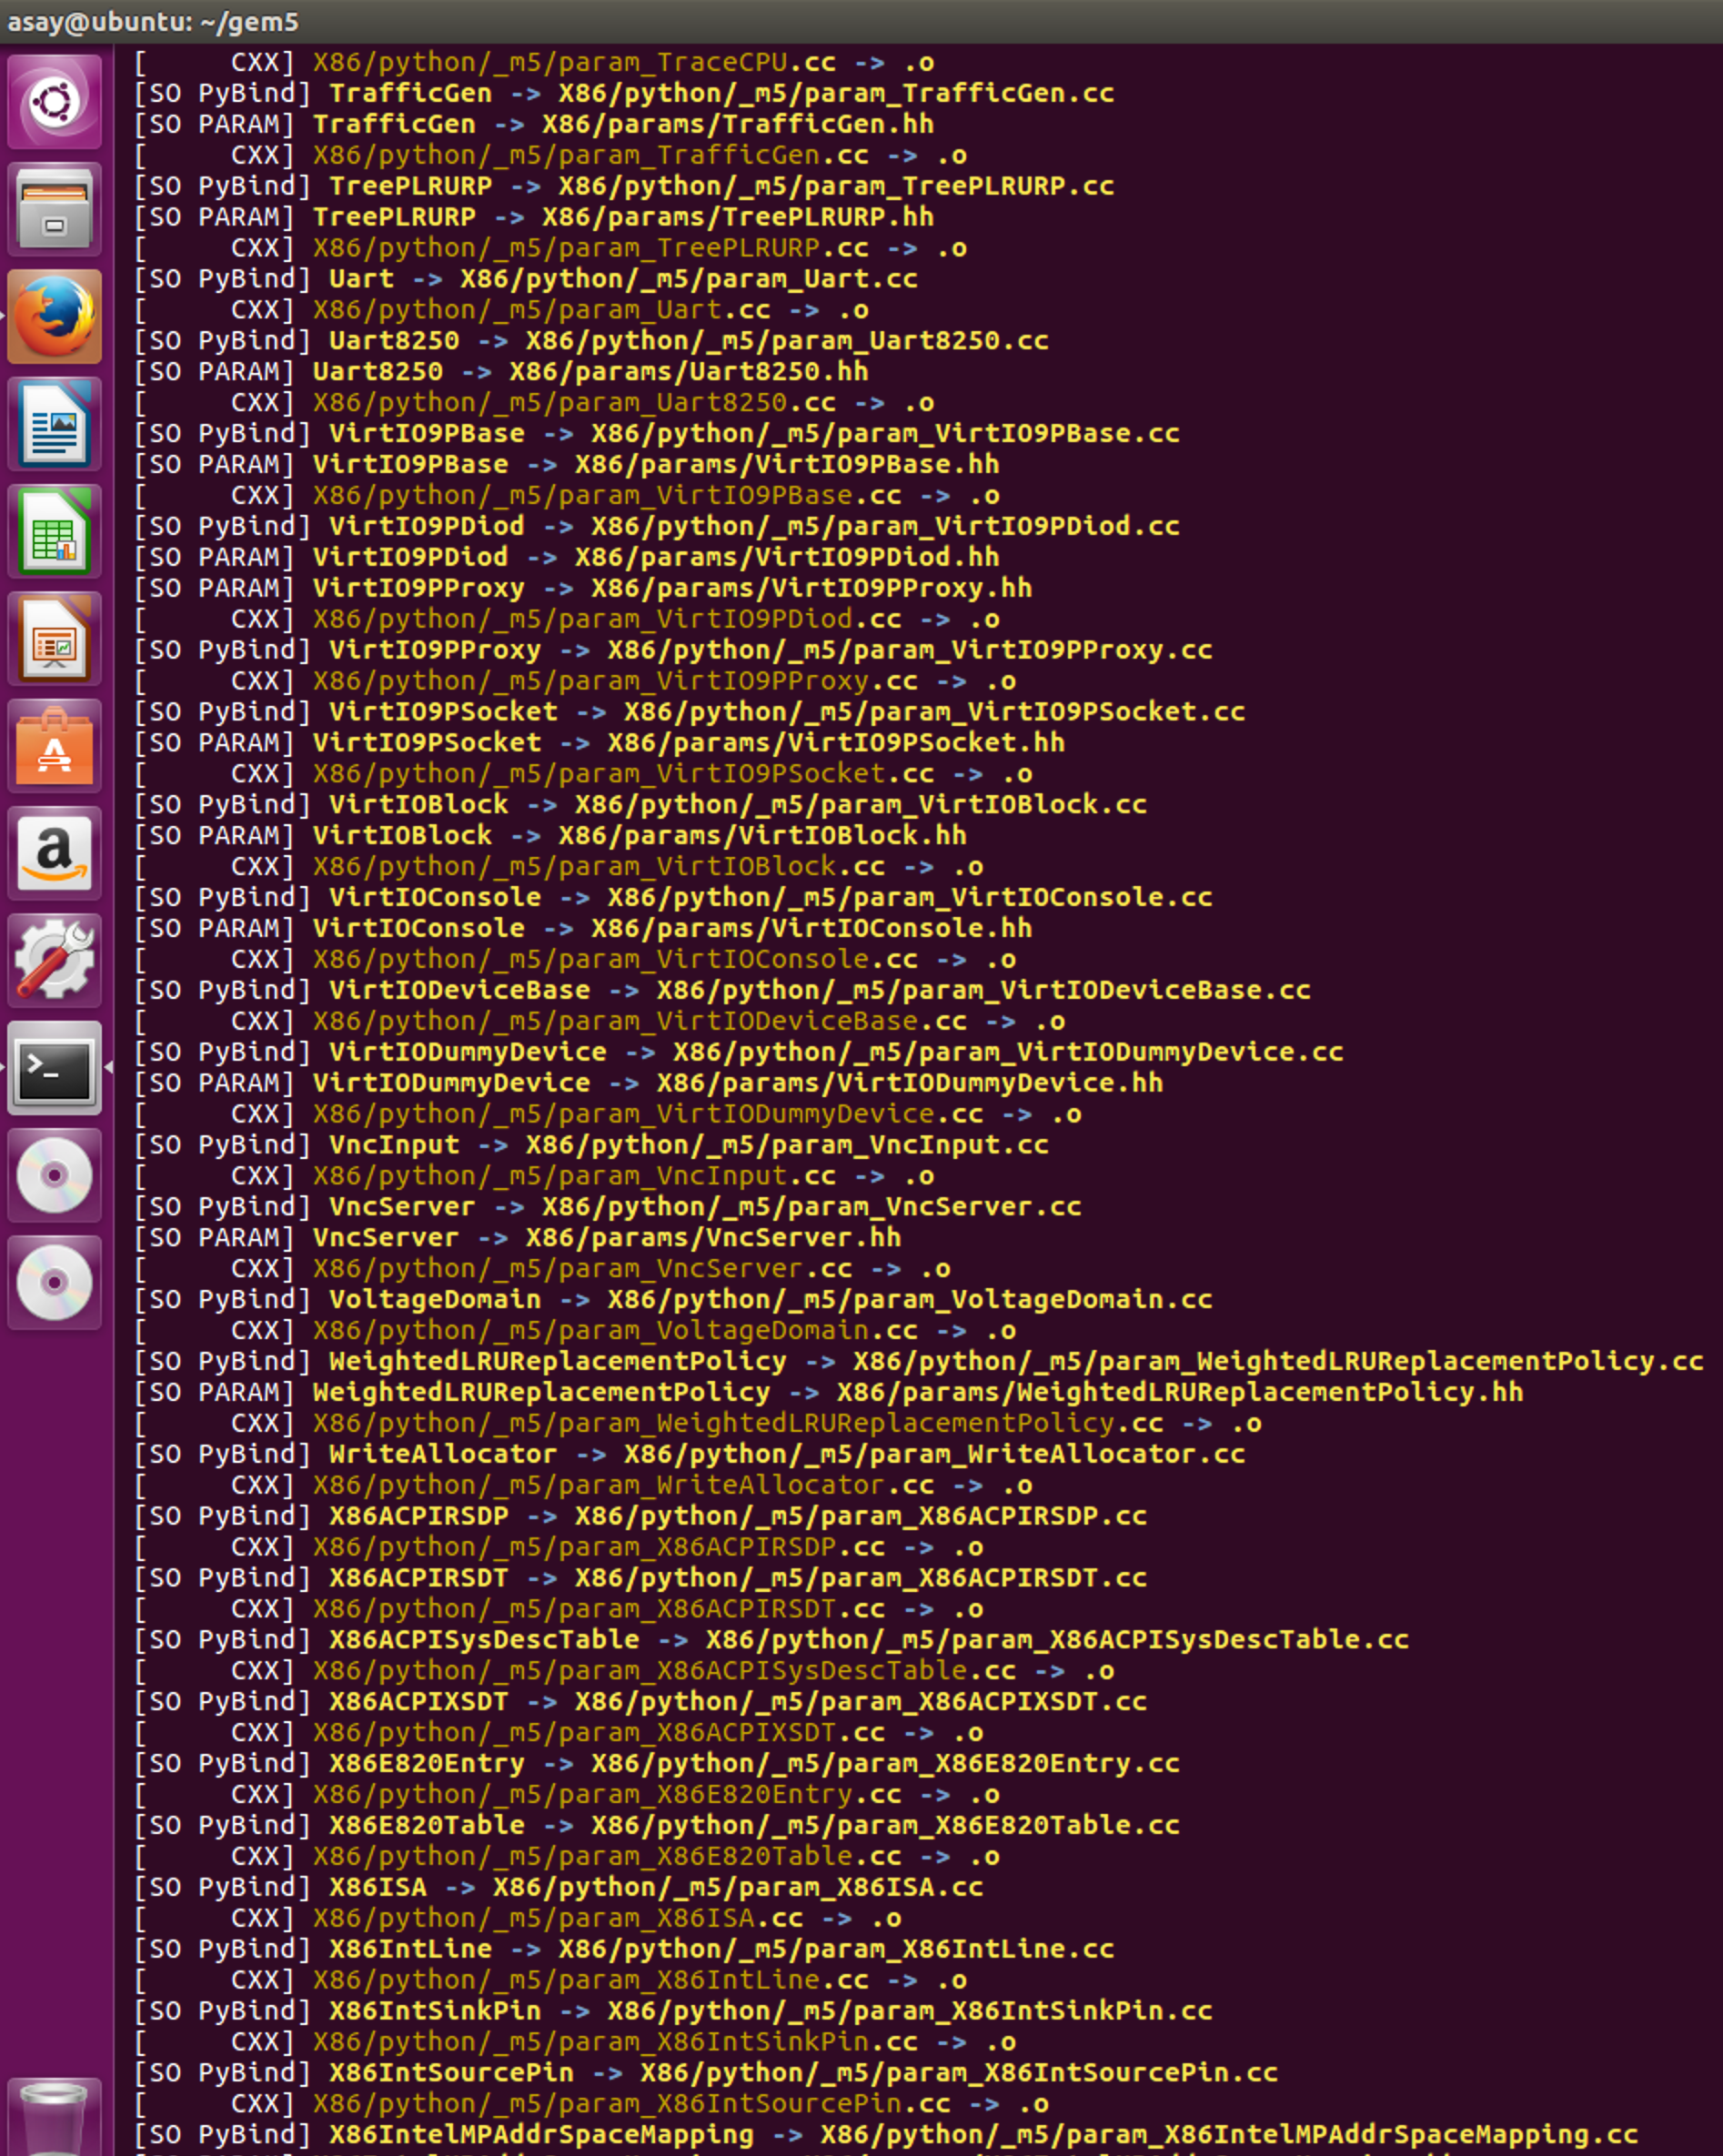
\includegraphics[width=1\textwidth]{build19}
%	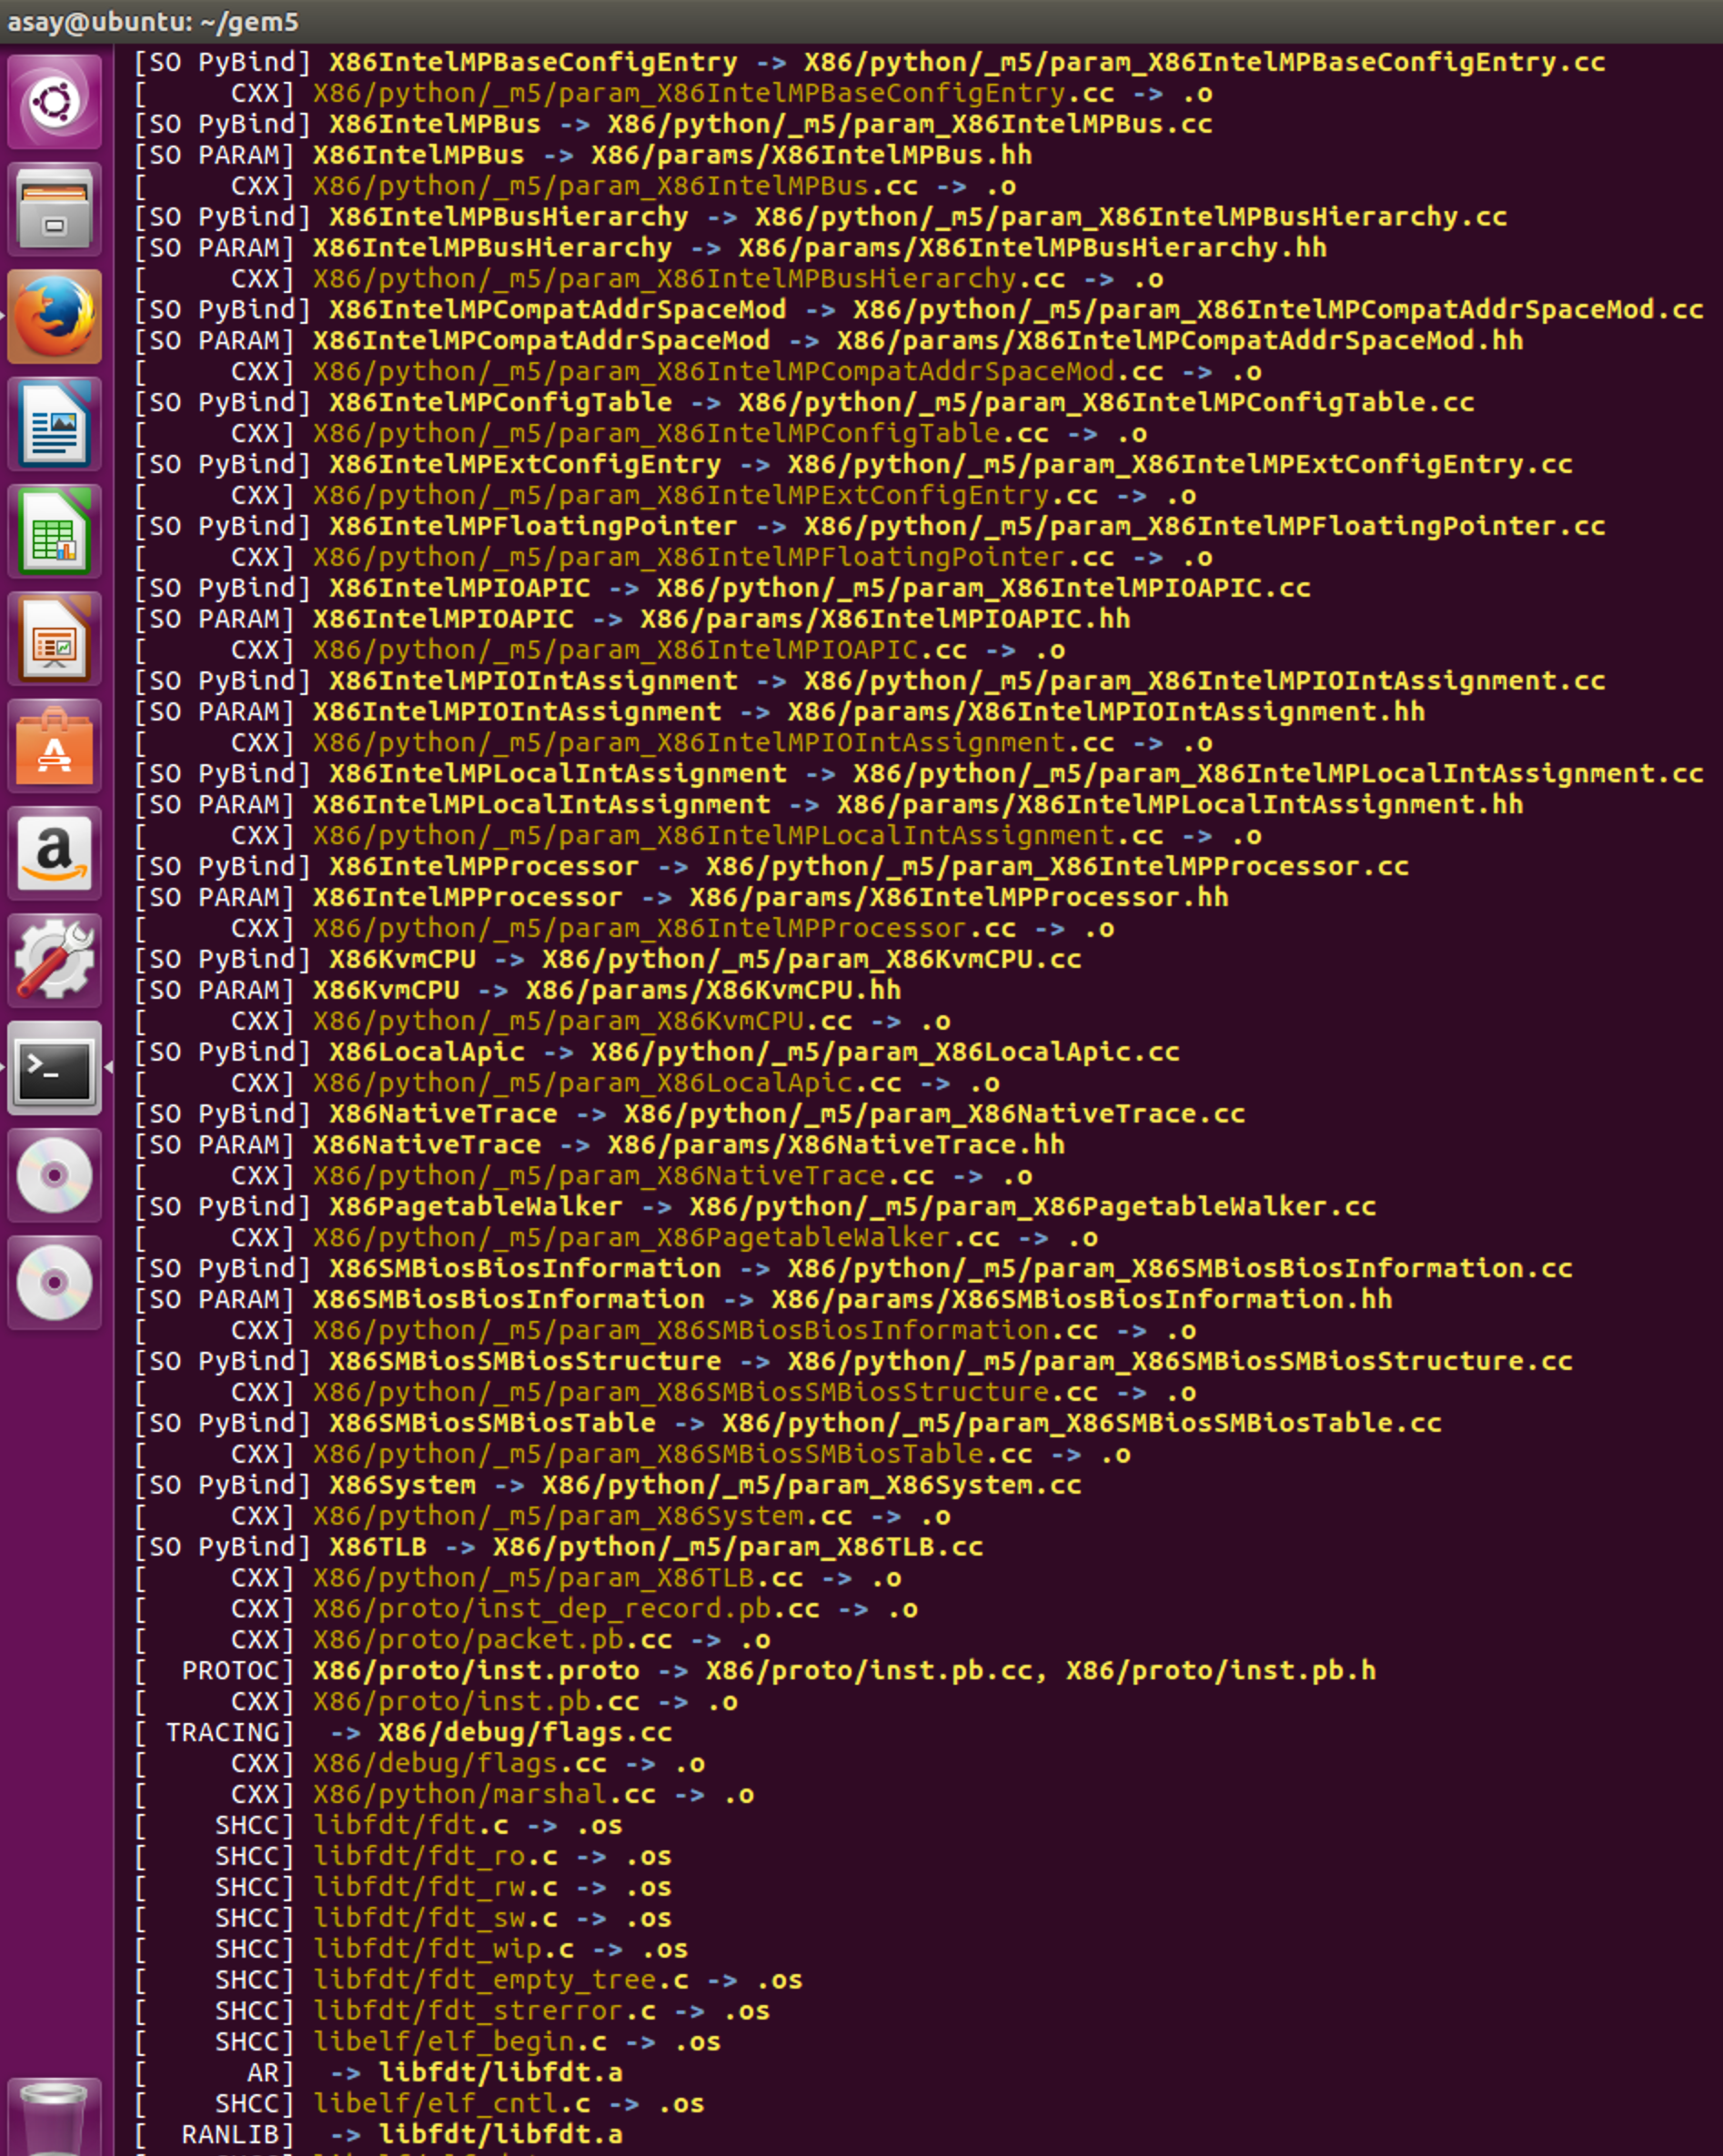
\includegraphics[width=1\textwidth]{build18}
%	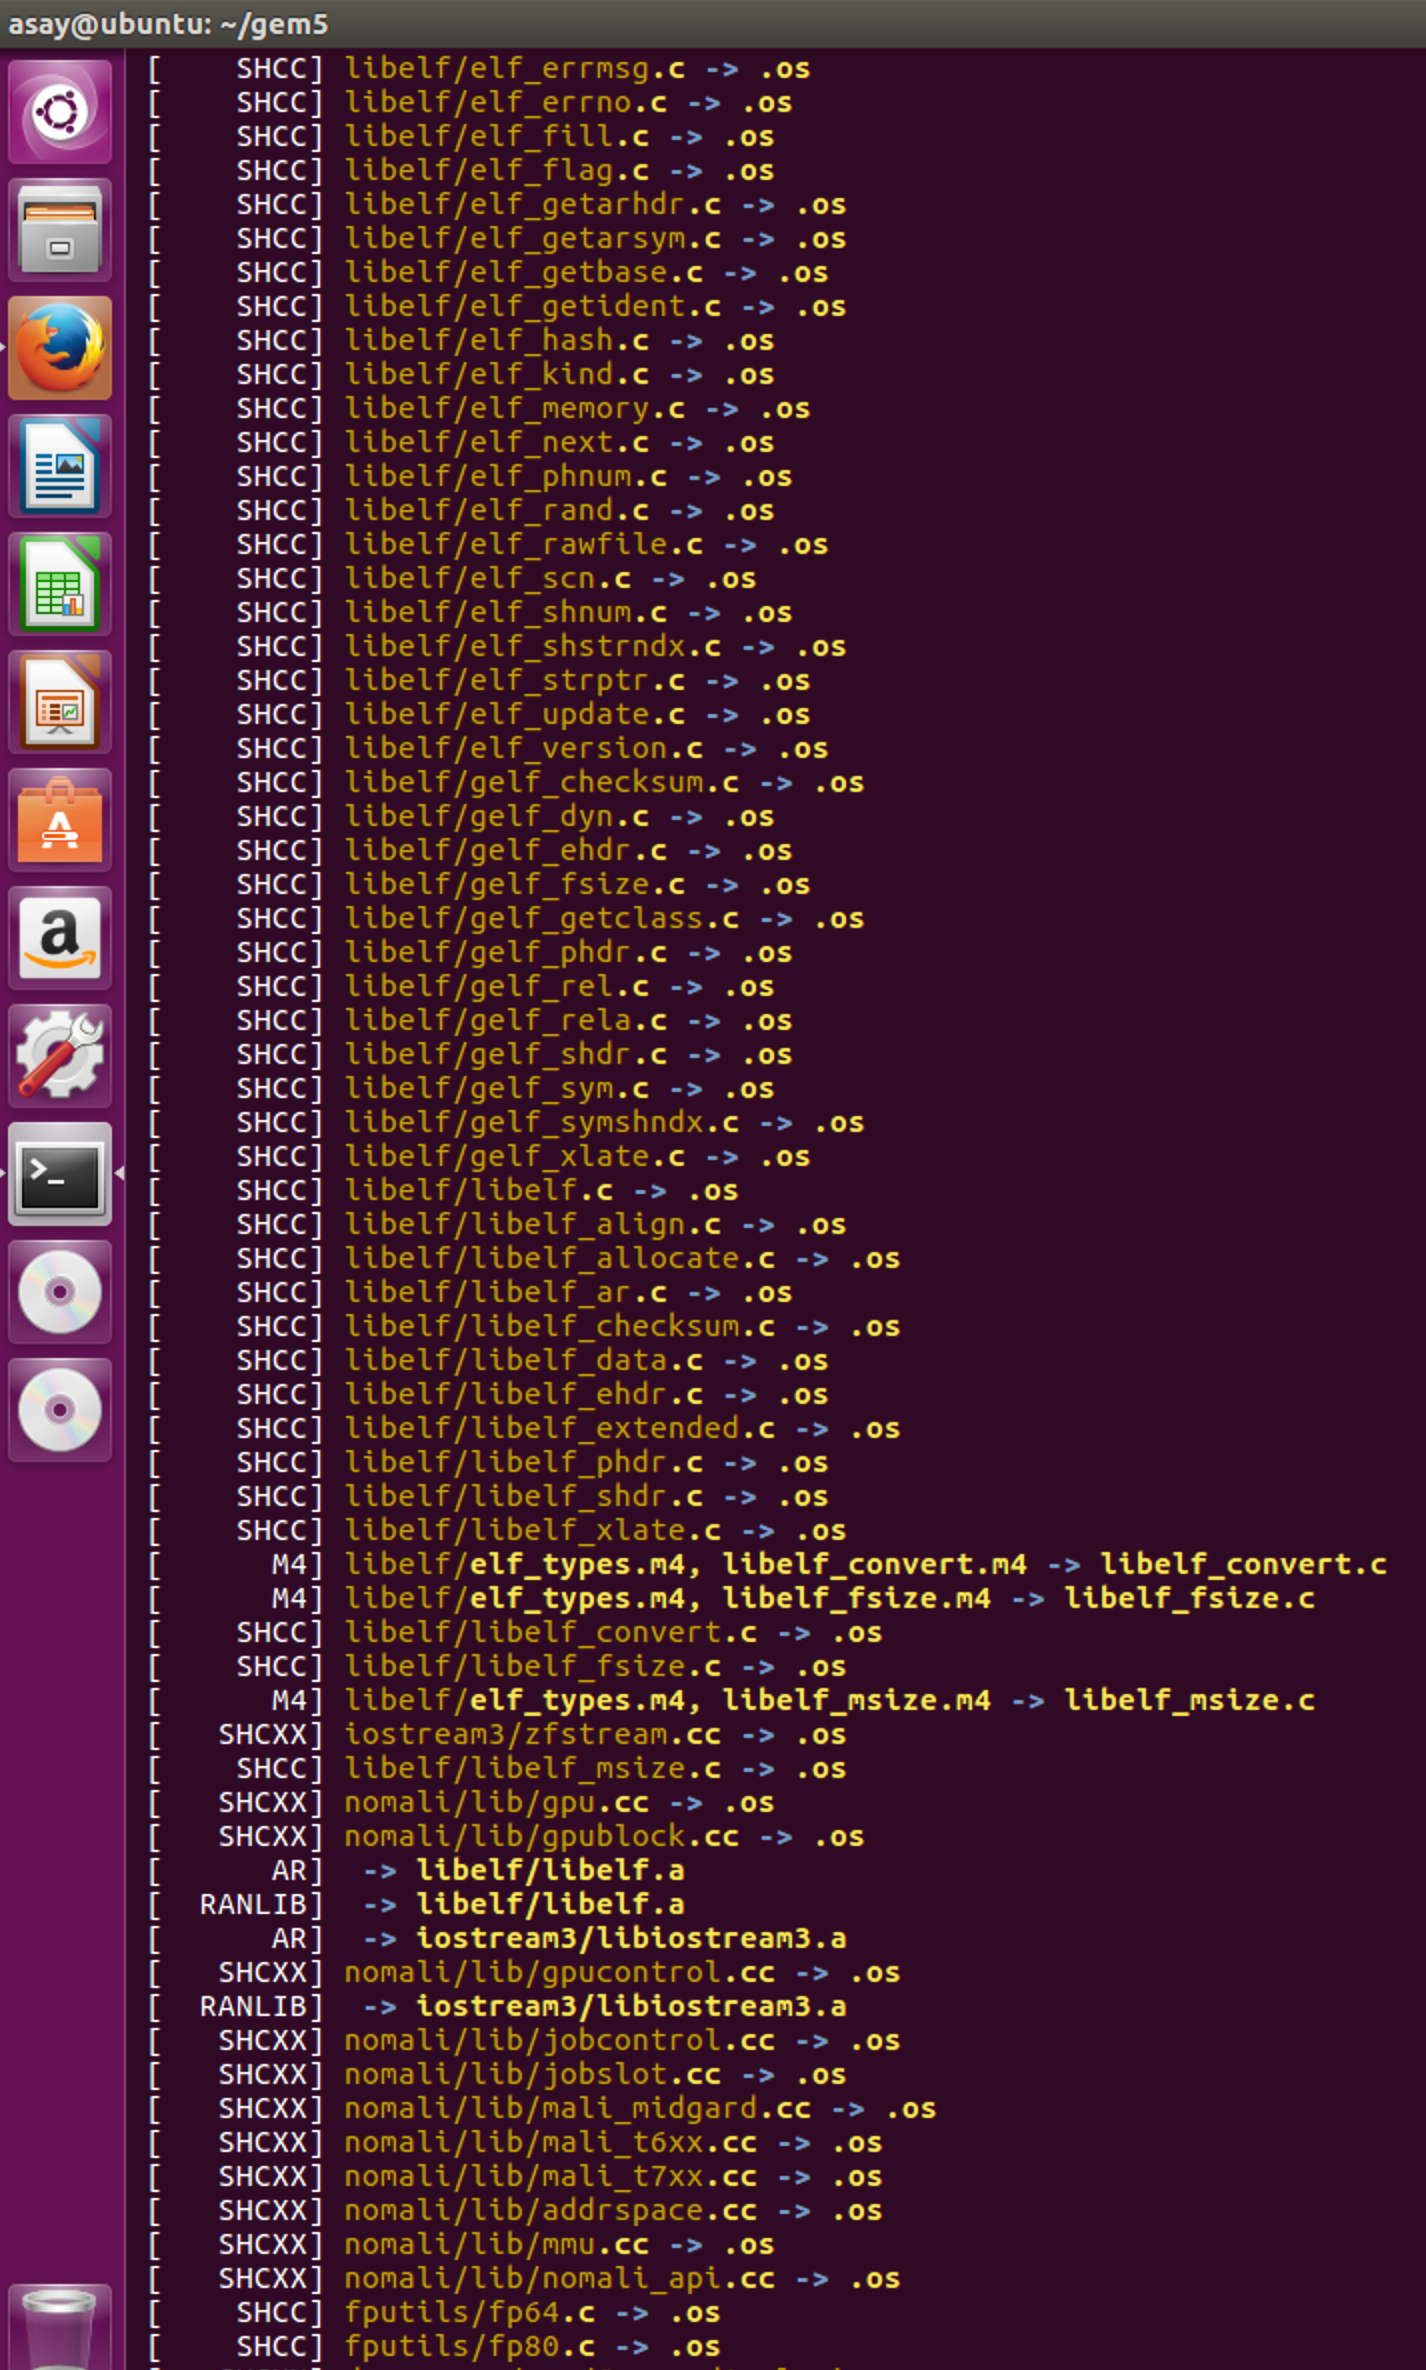
\includegraphics[width=1\textwidth]{build17}
%	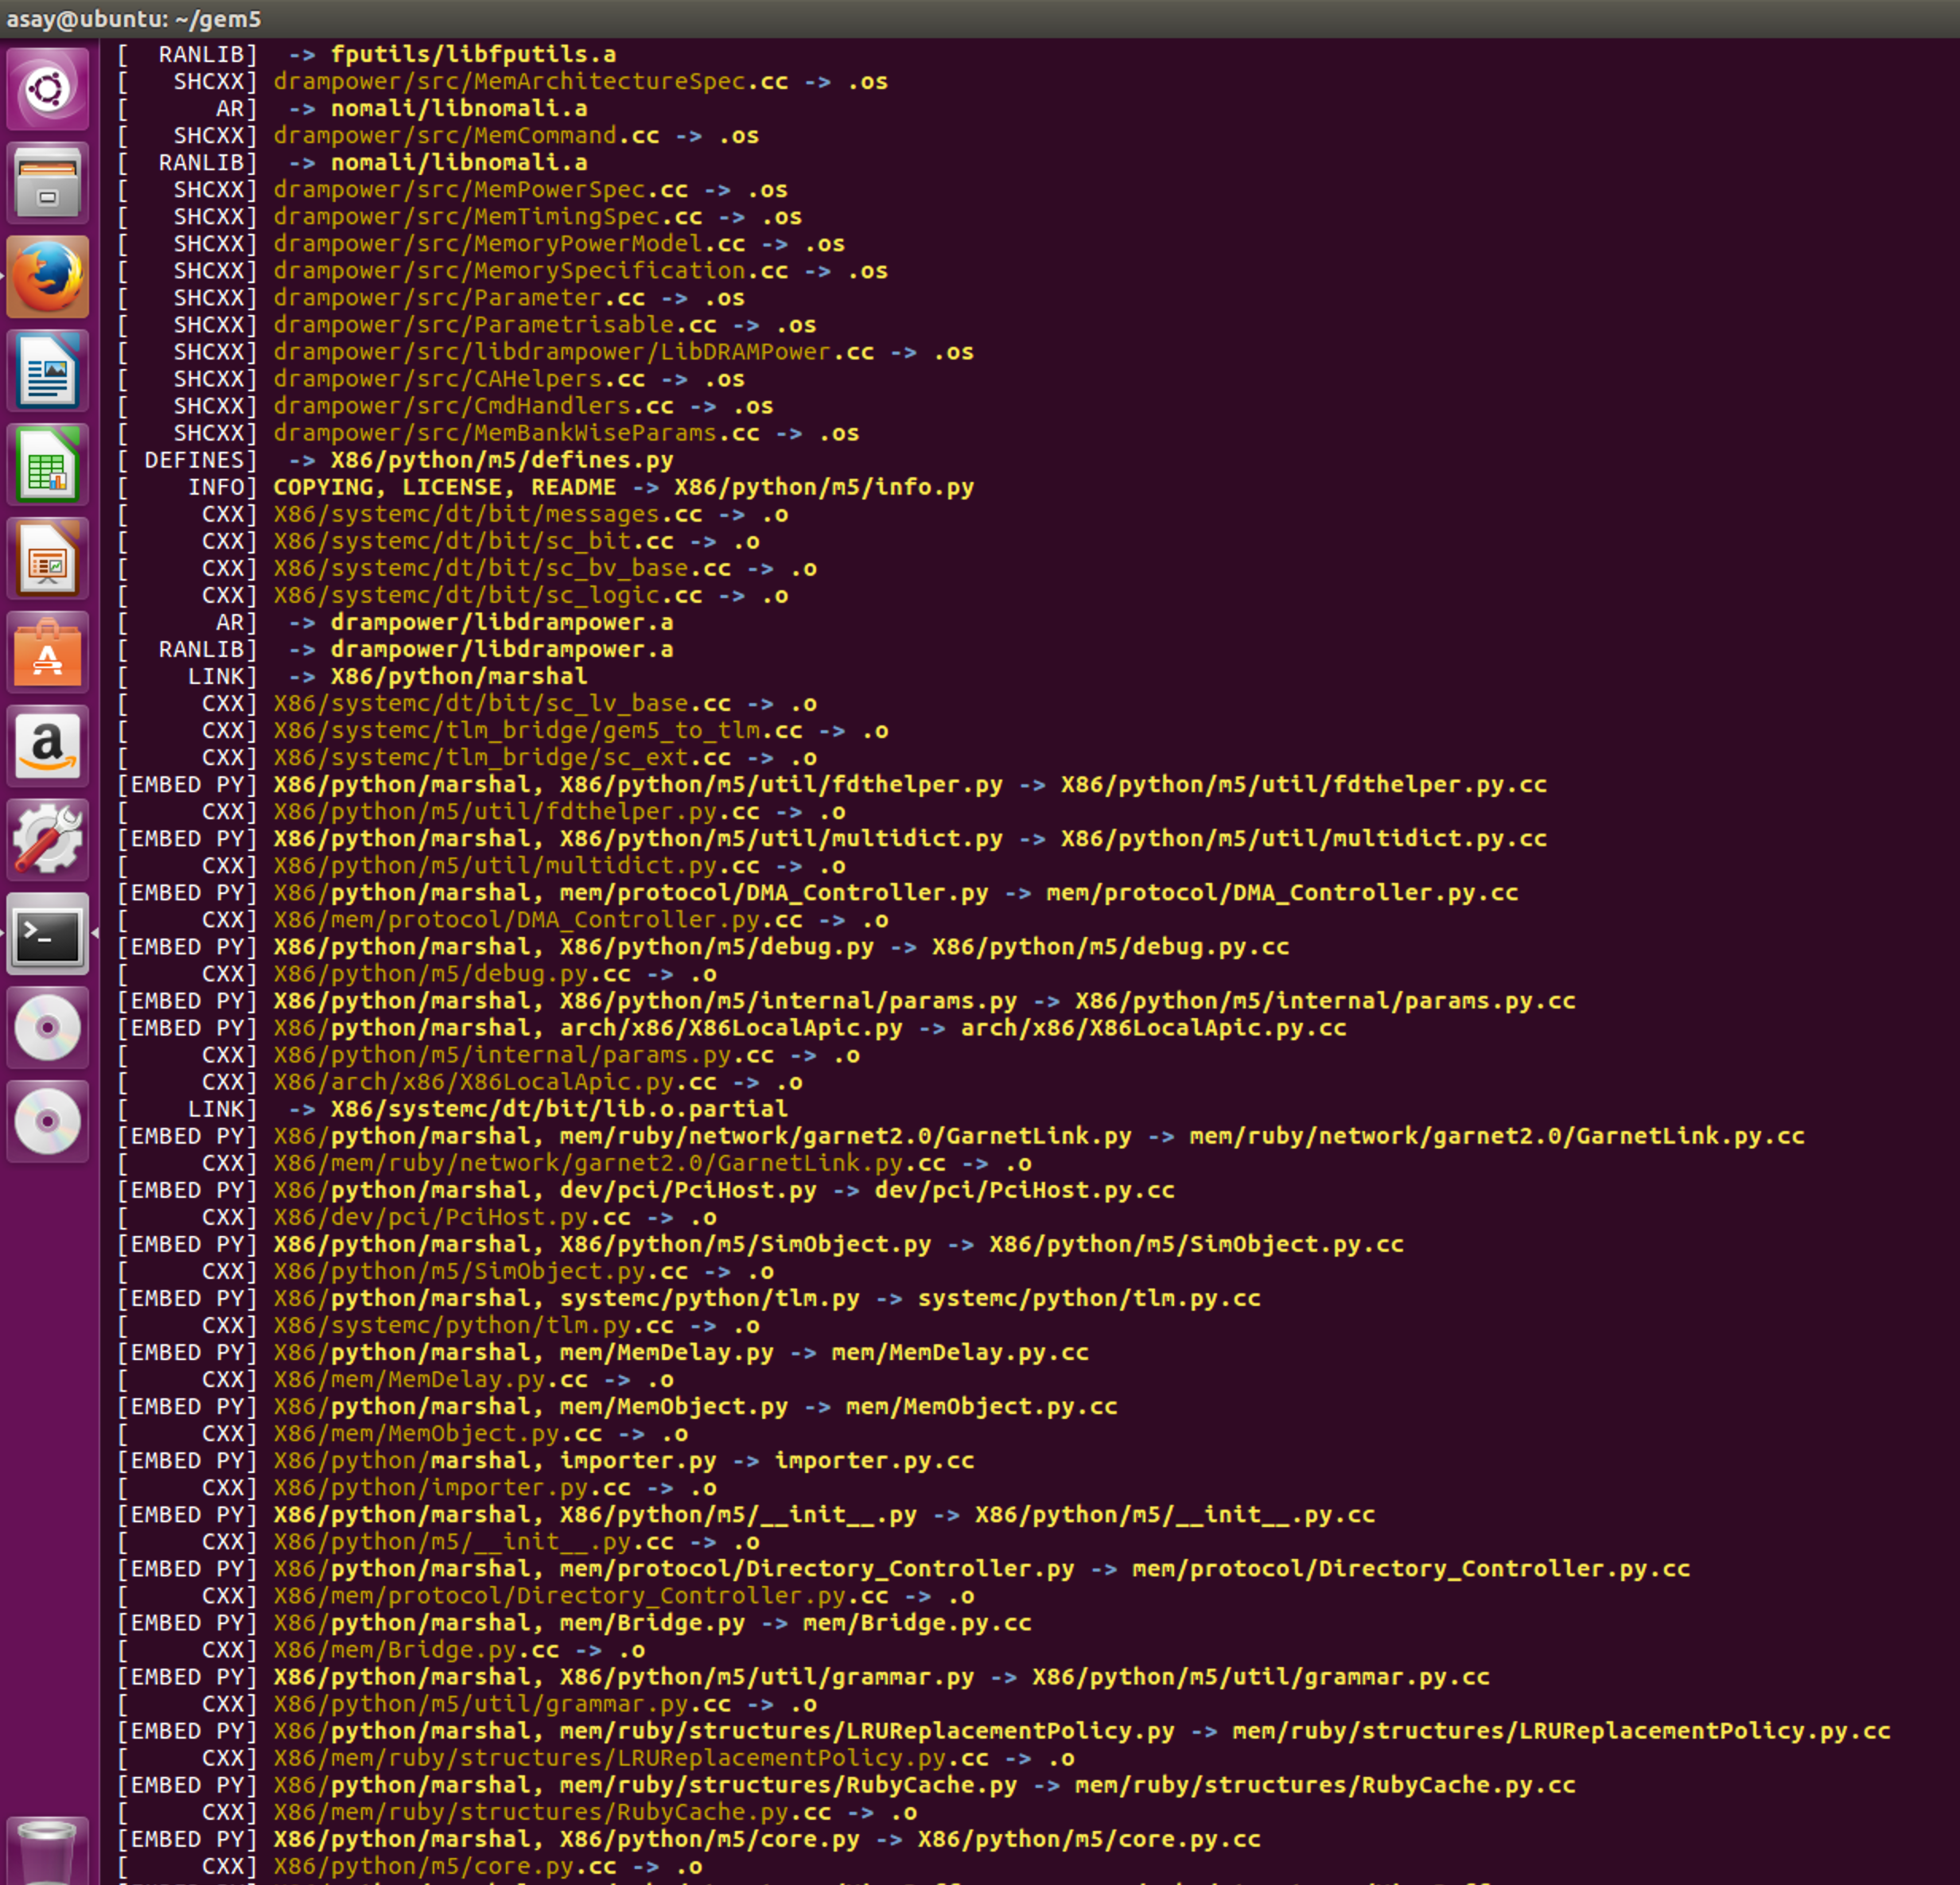
\includegraphics[width=1\textwidth]{build16}
%	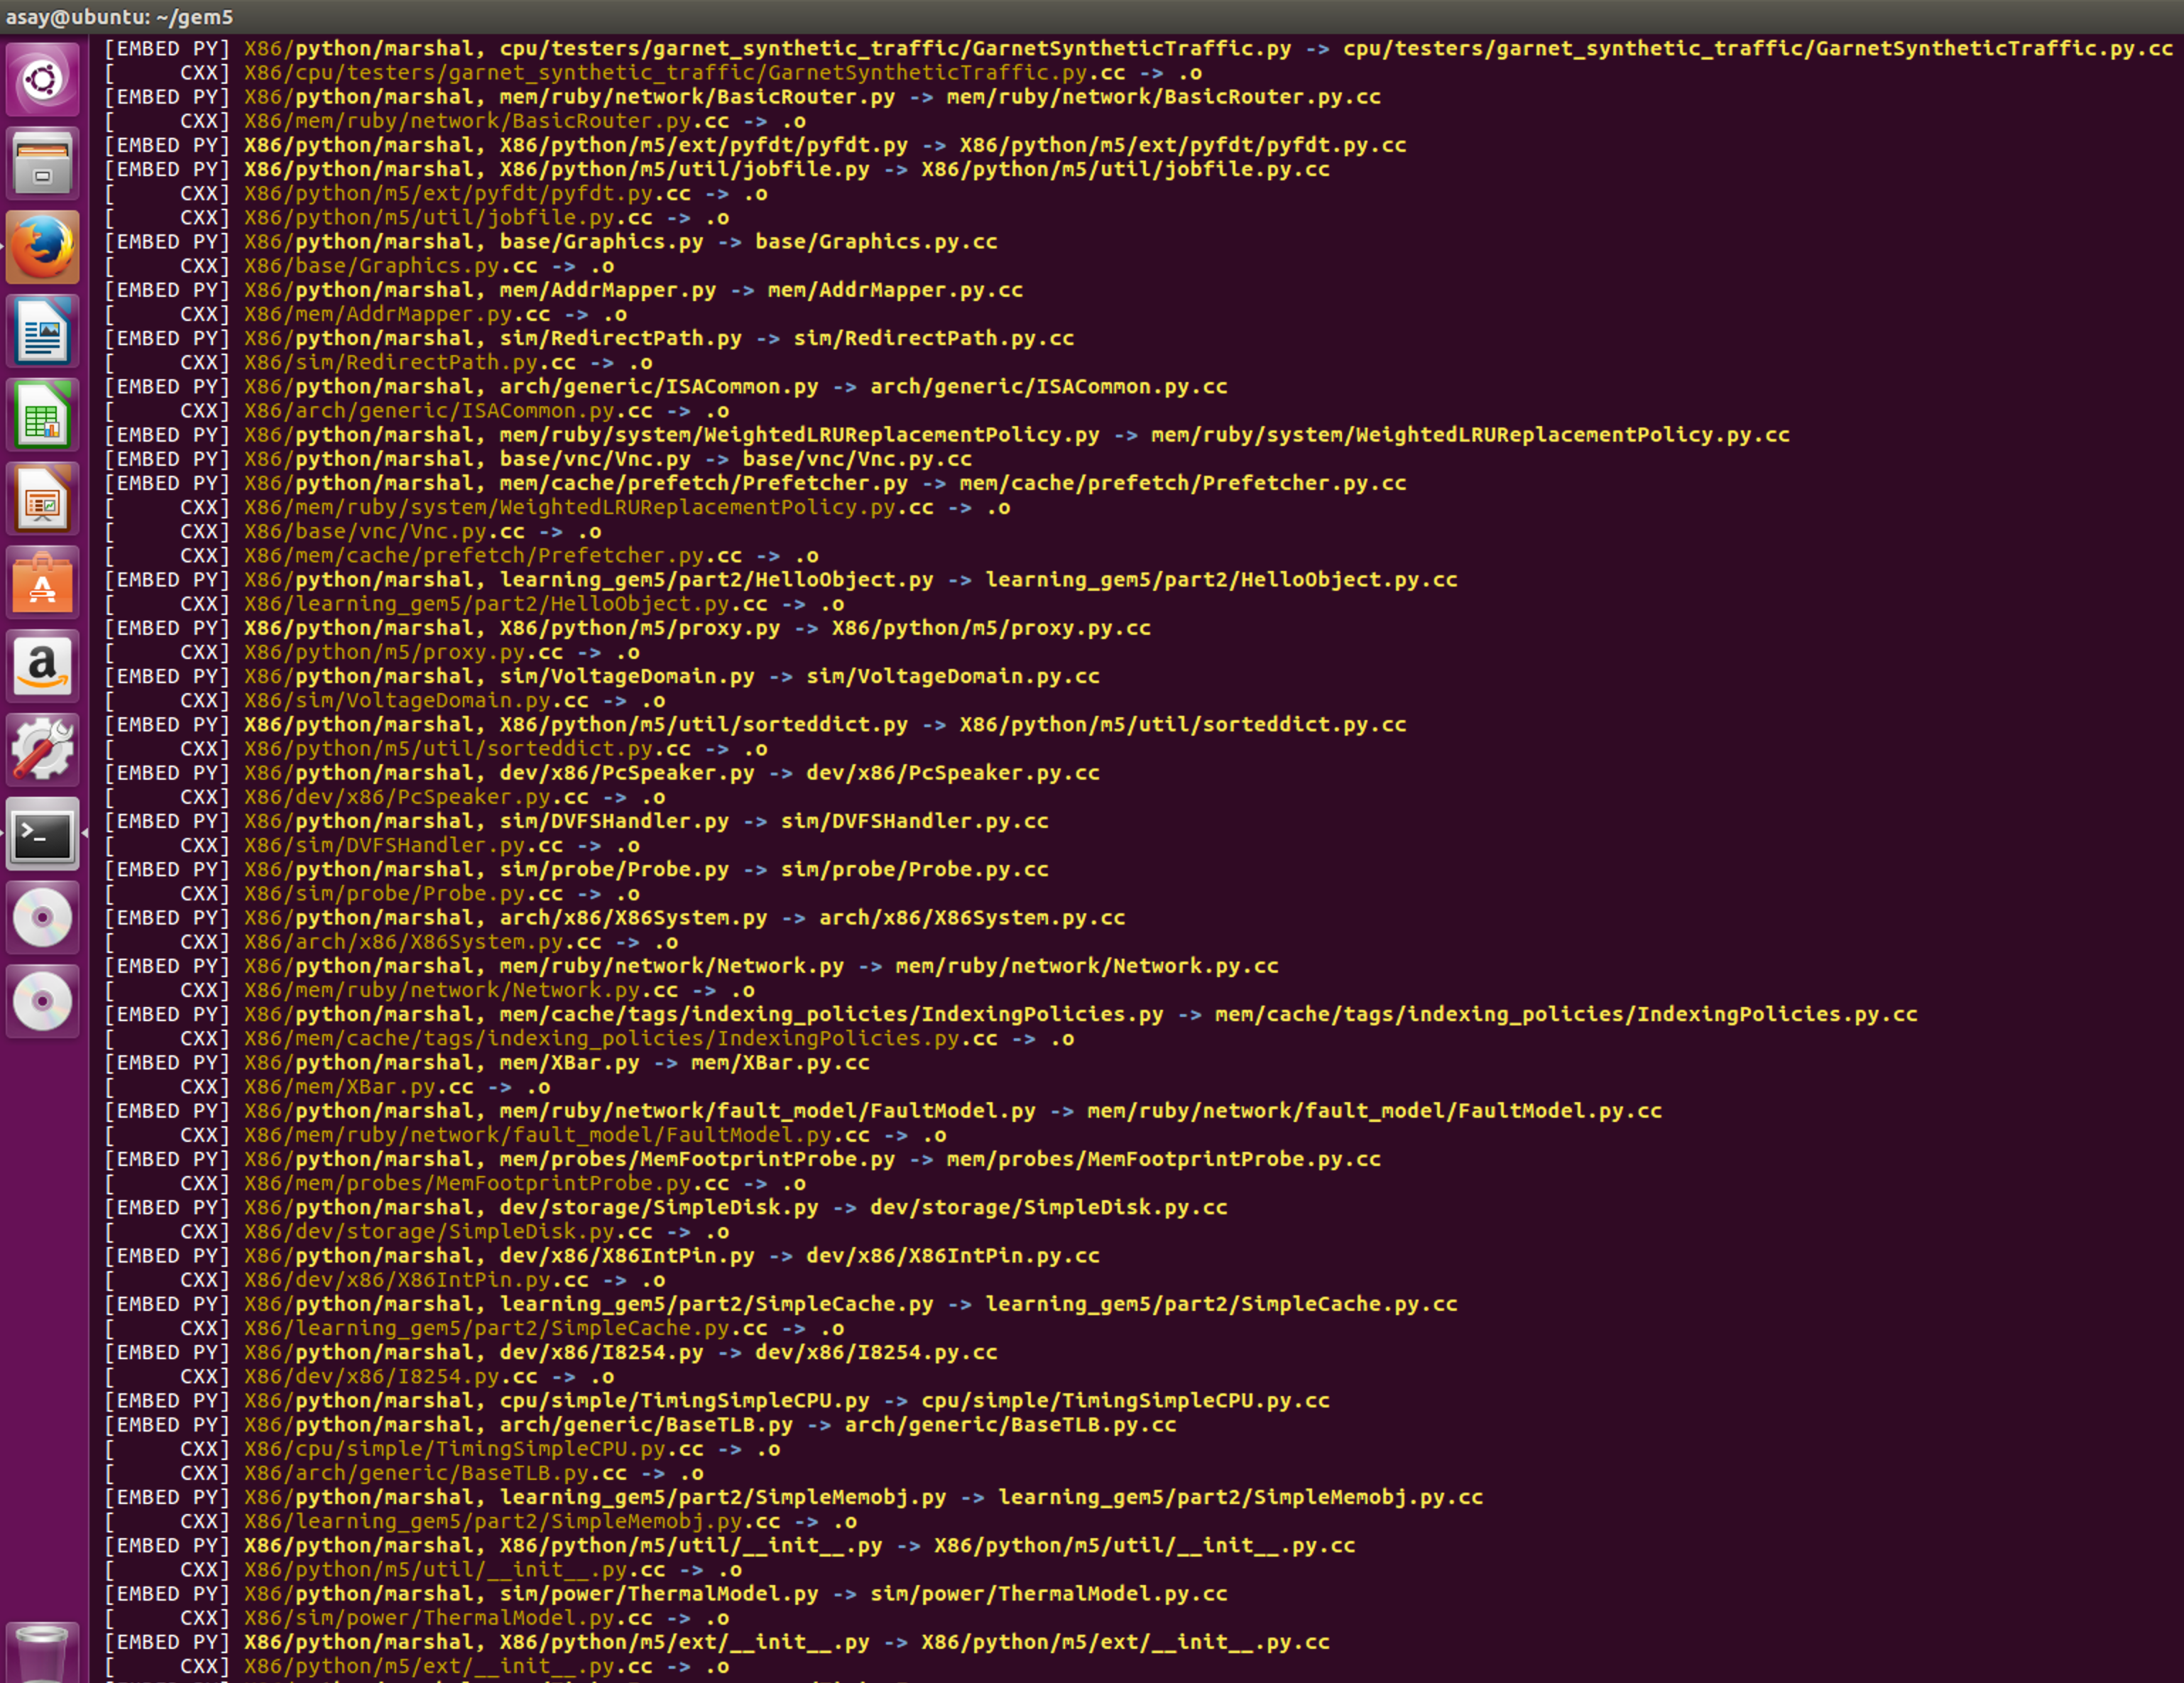
\includegraphics[width=1\textwidth]{build15}
%	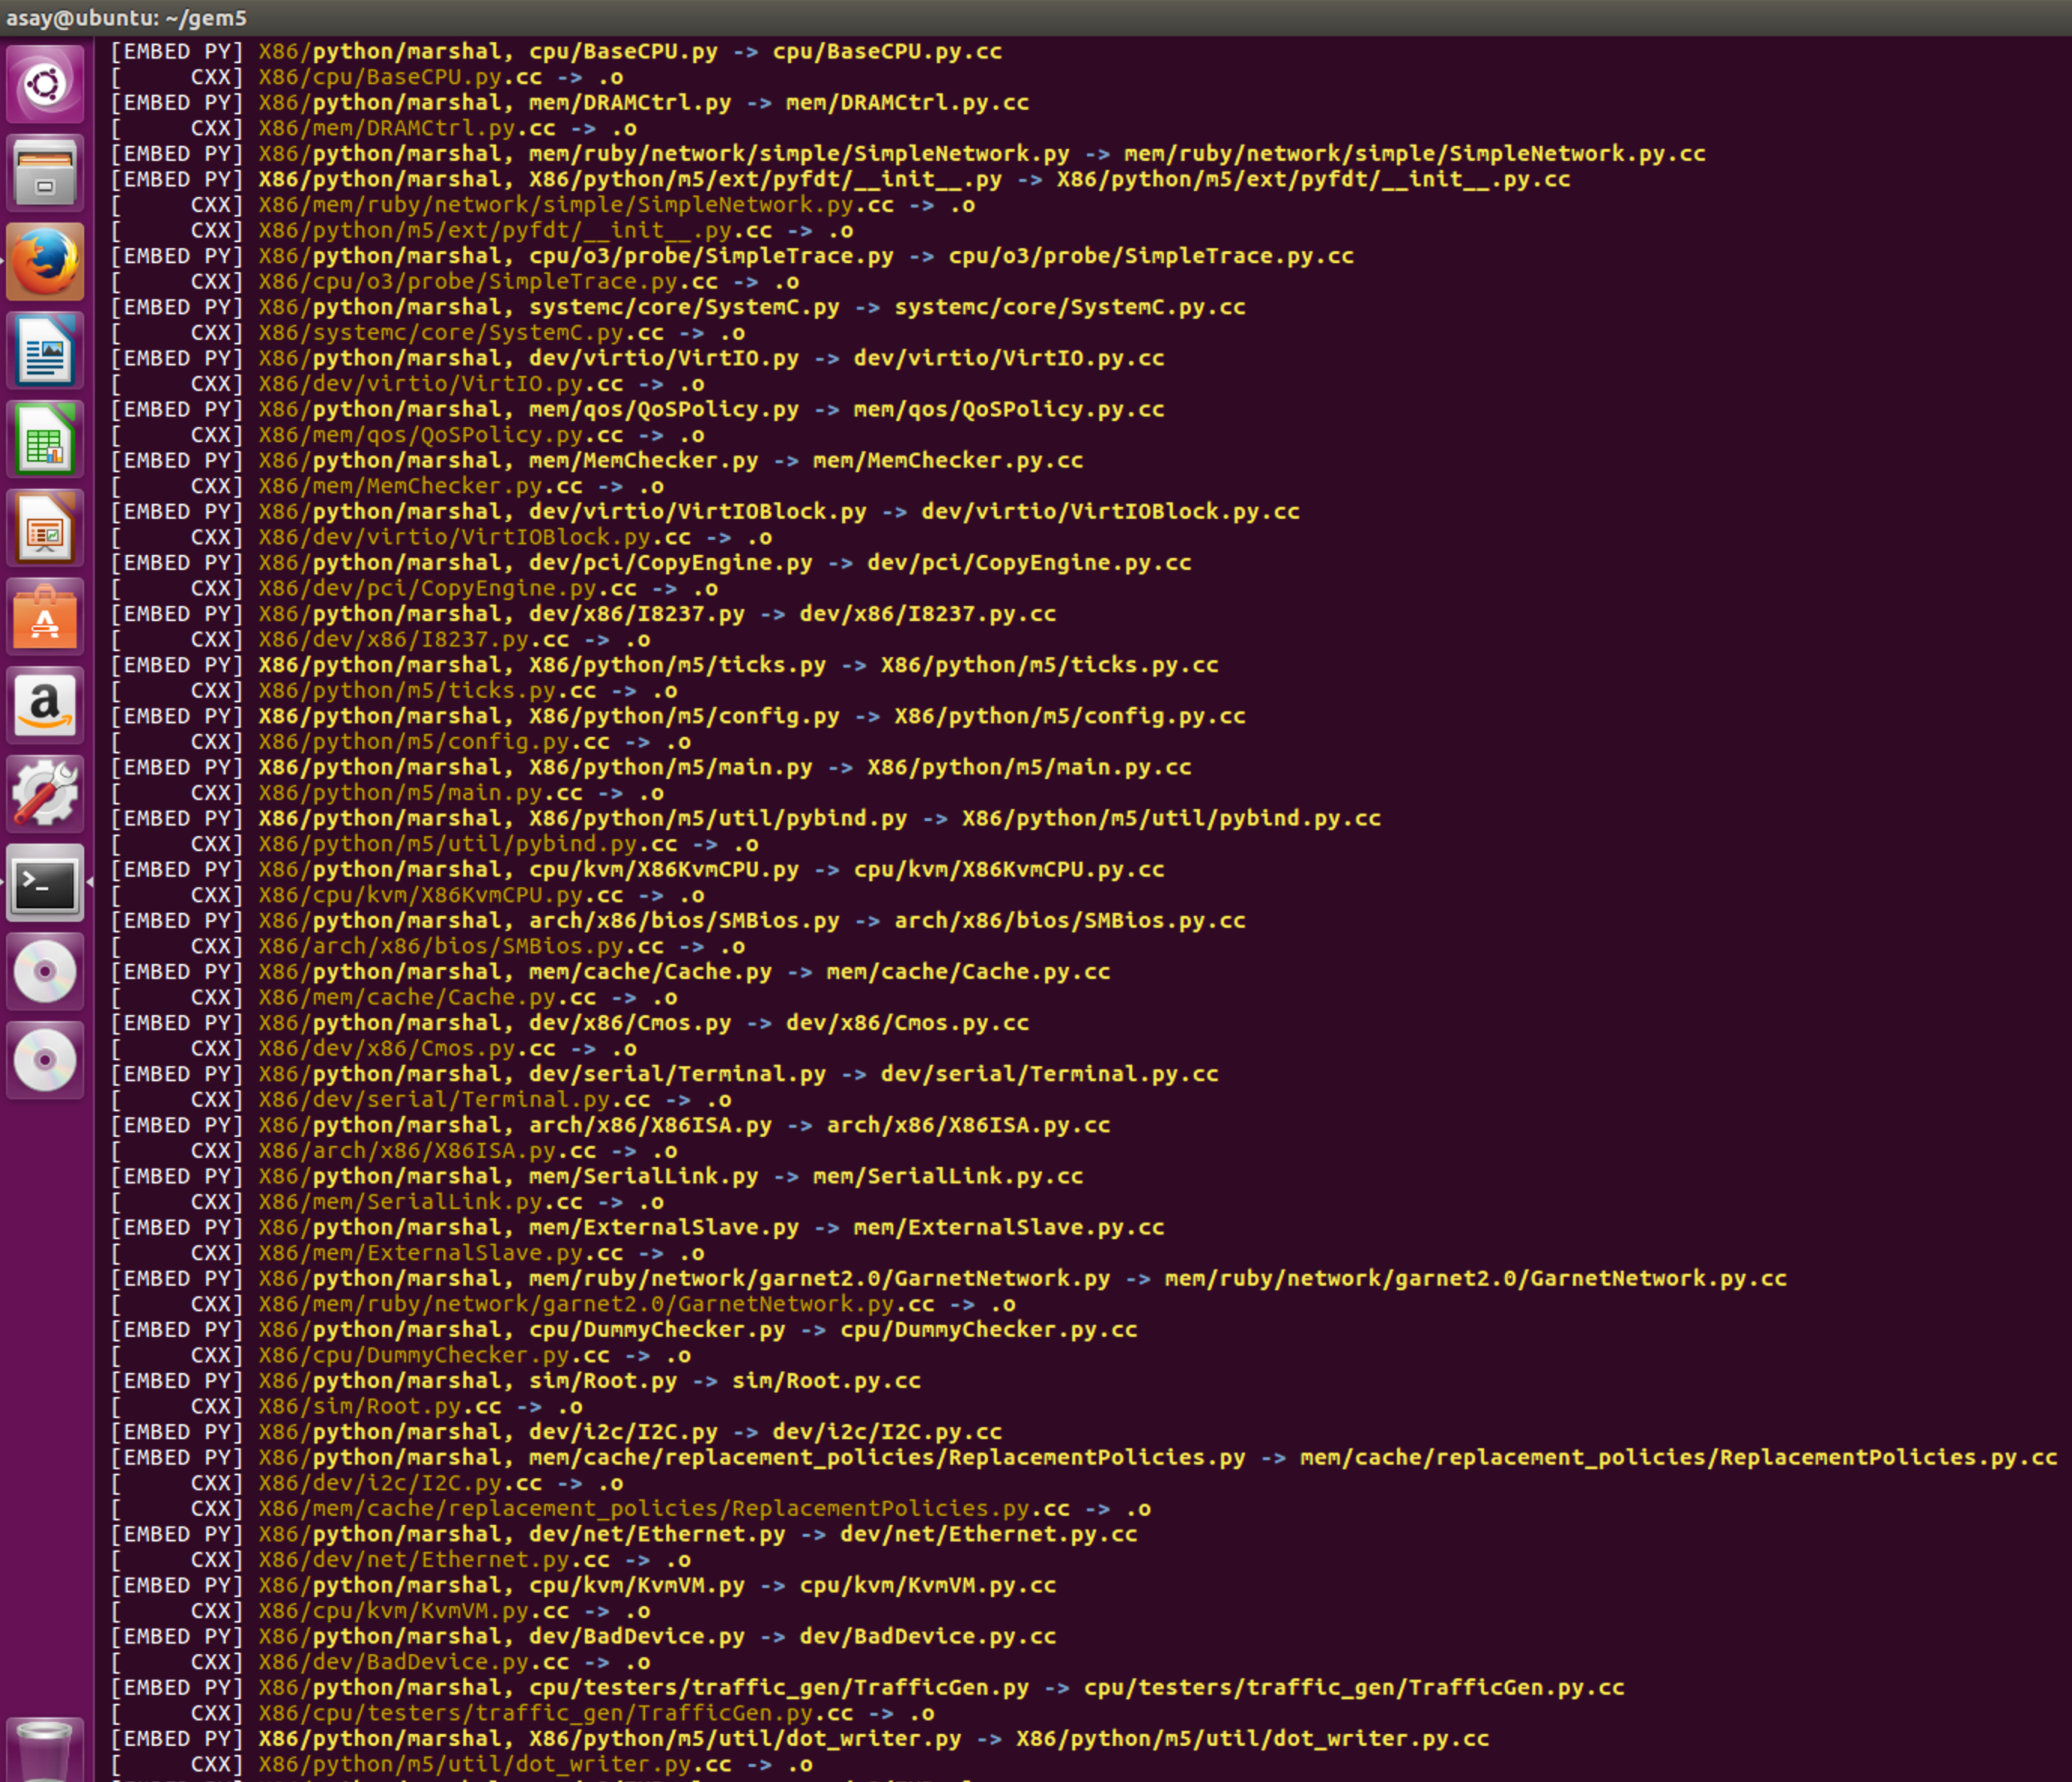
\includegraphics[width=1\textwidth]{build14}
%	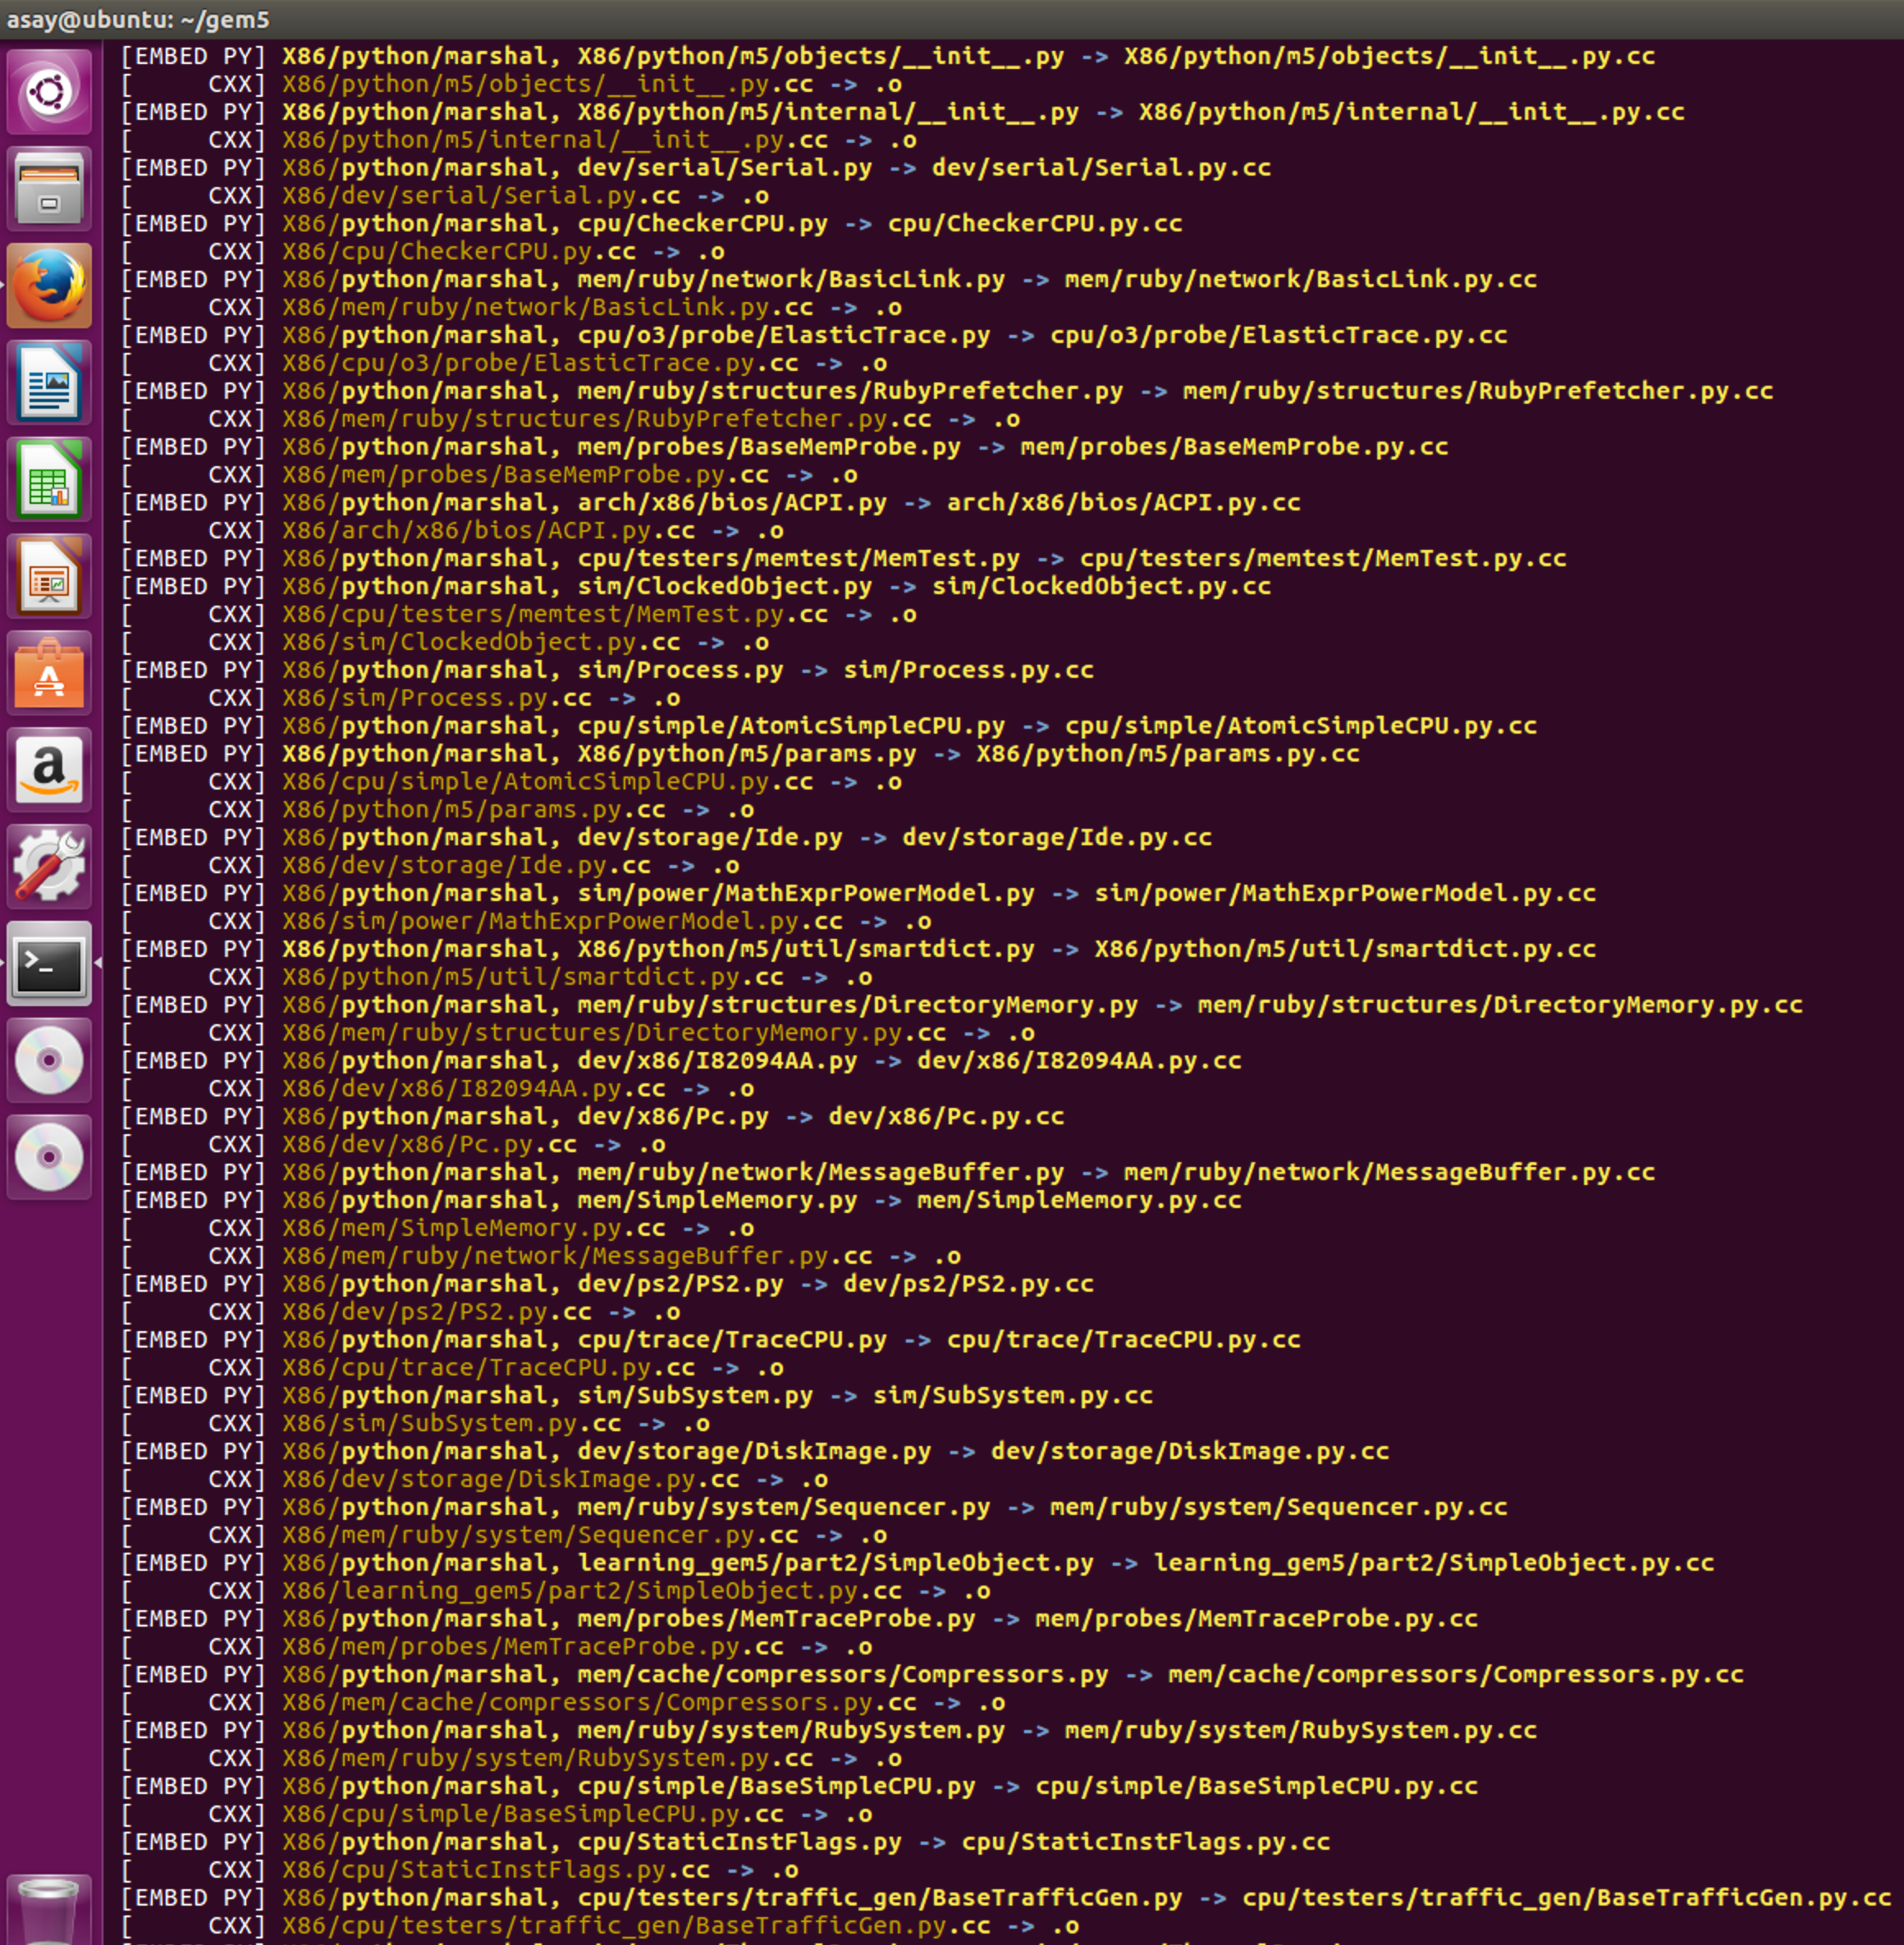
\includegraphics[width=1\textwidth]{build13}
%	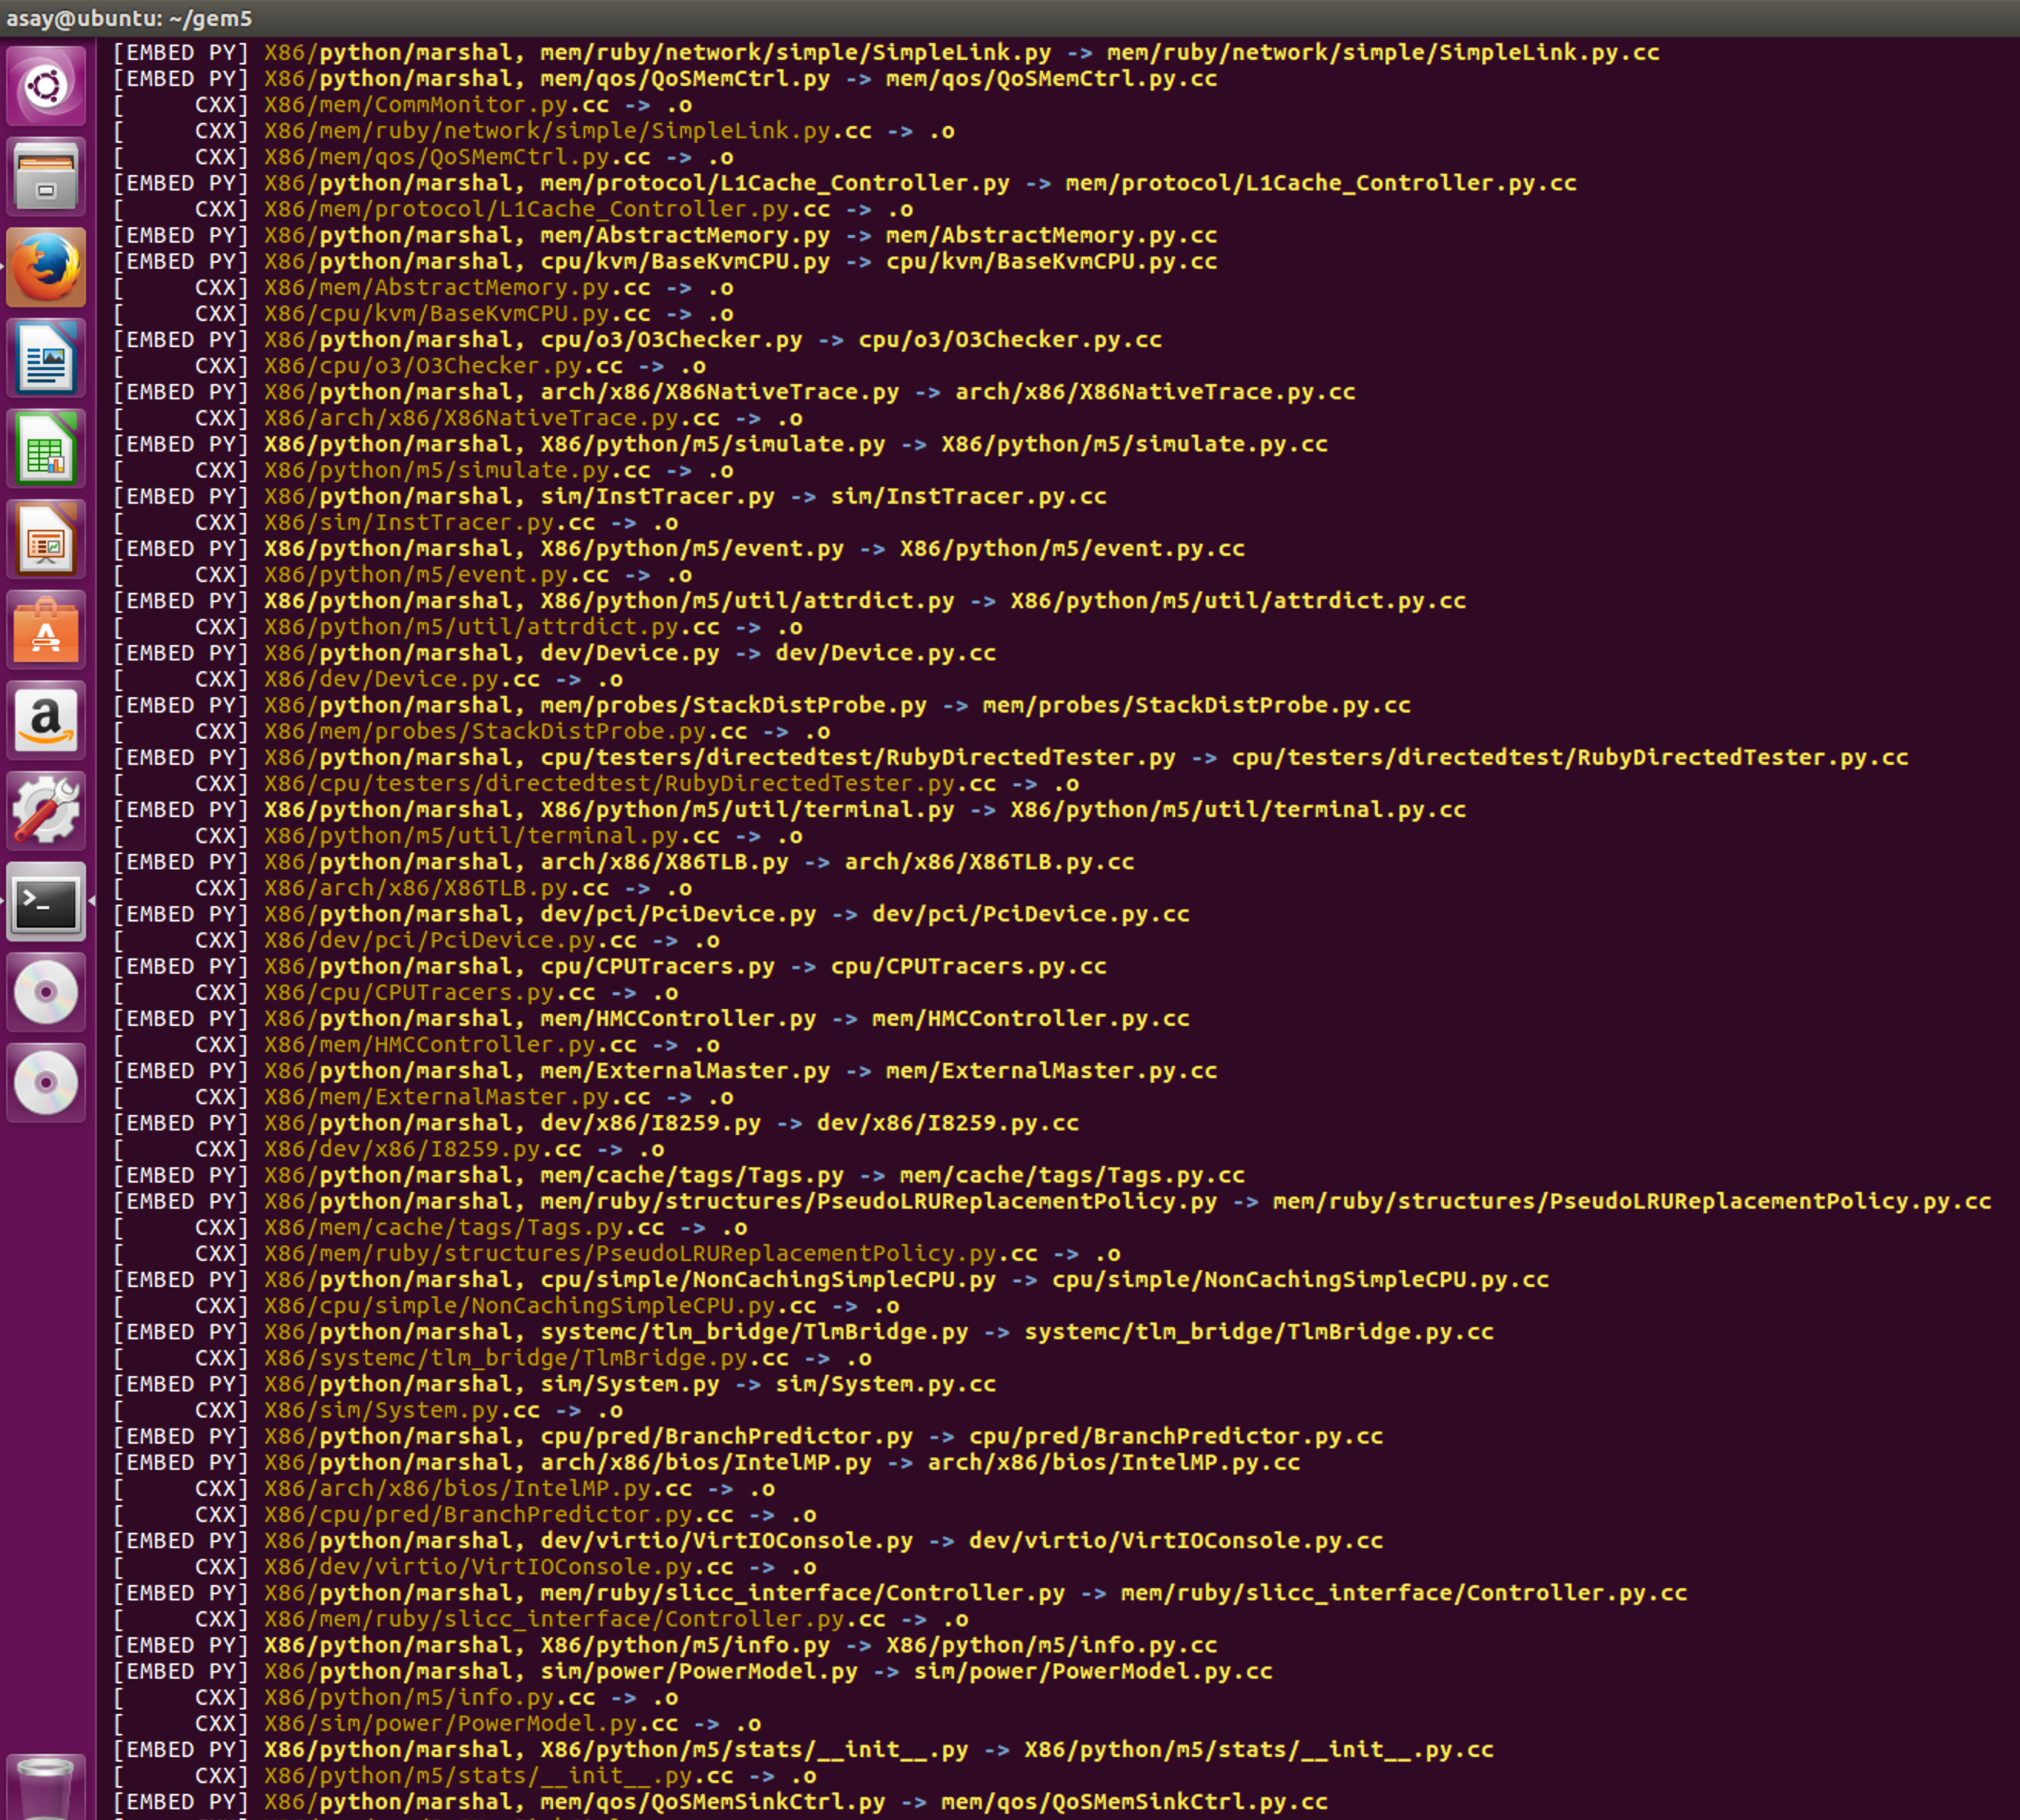
\includegraphics[width=1\textwidth]{build12}
%	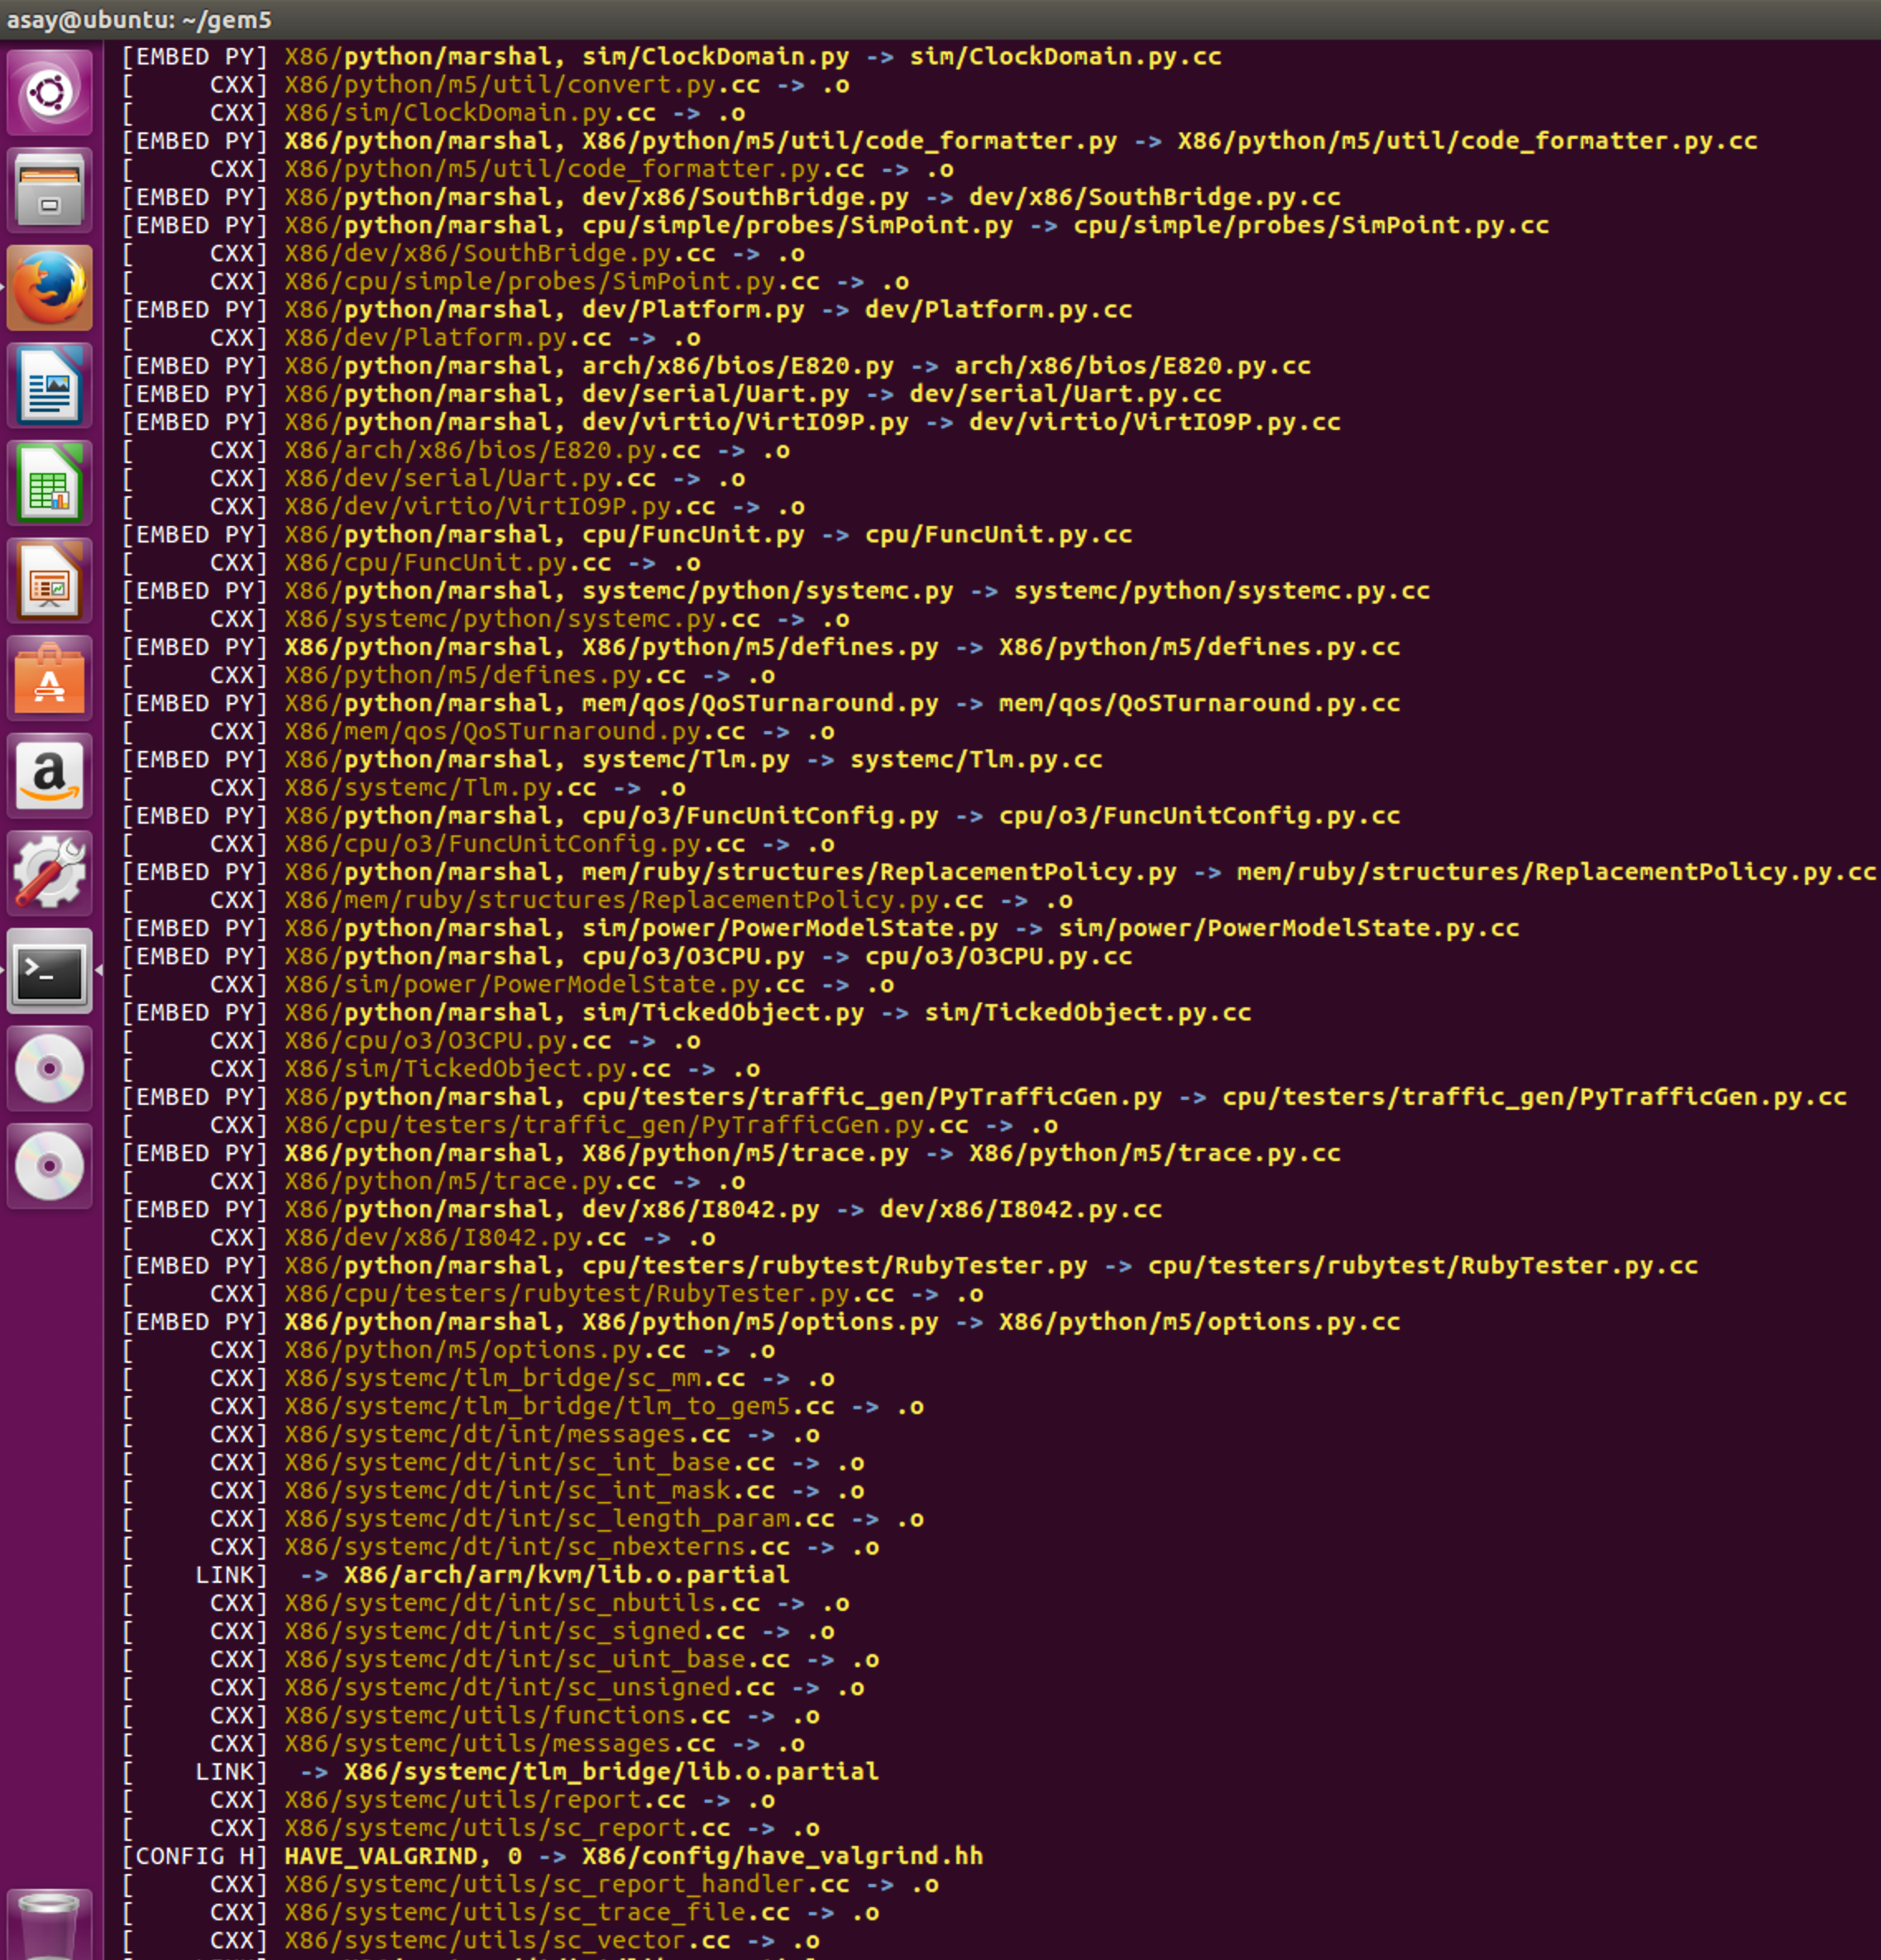
\includegraphics[width=1\textwidth]{build11}
%	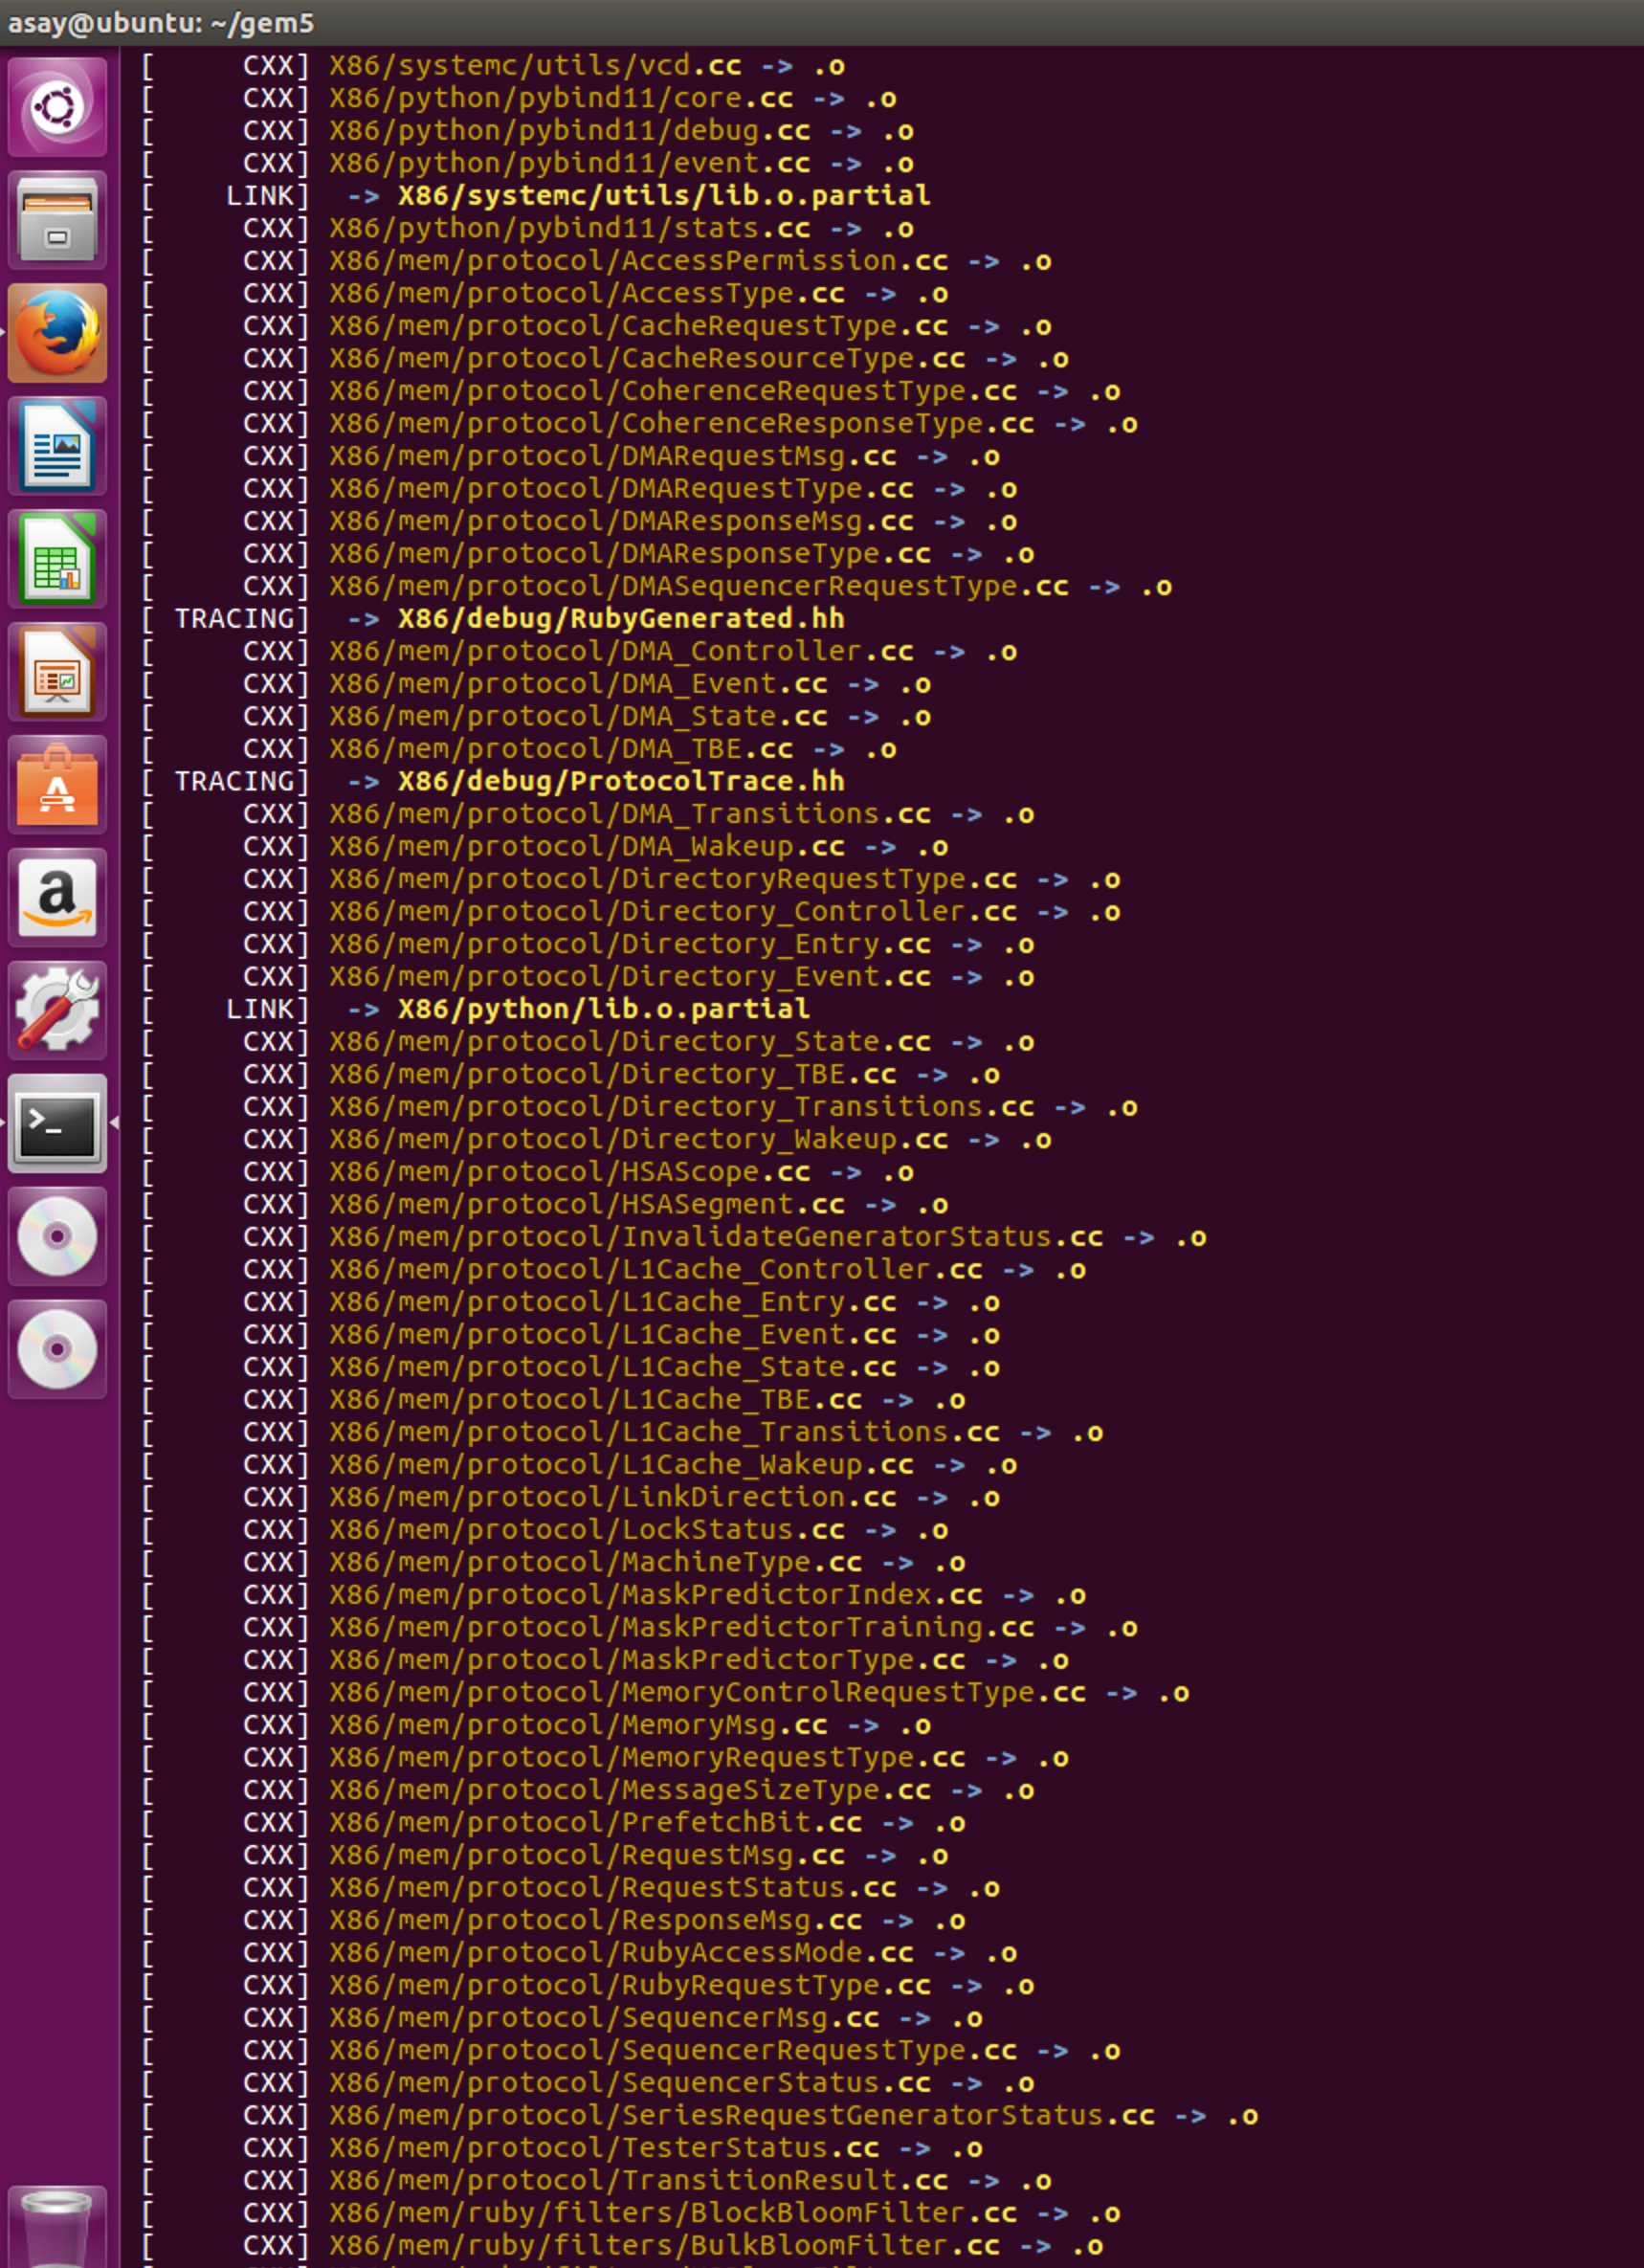
\includegraphics[width=1\textwidth]{build10}
%	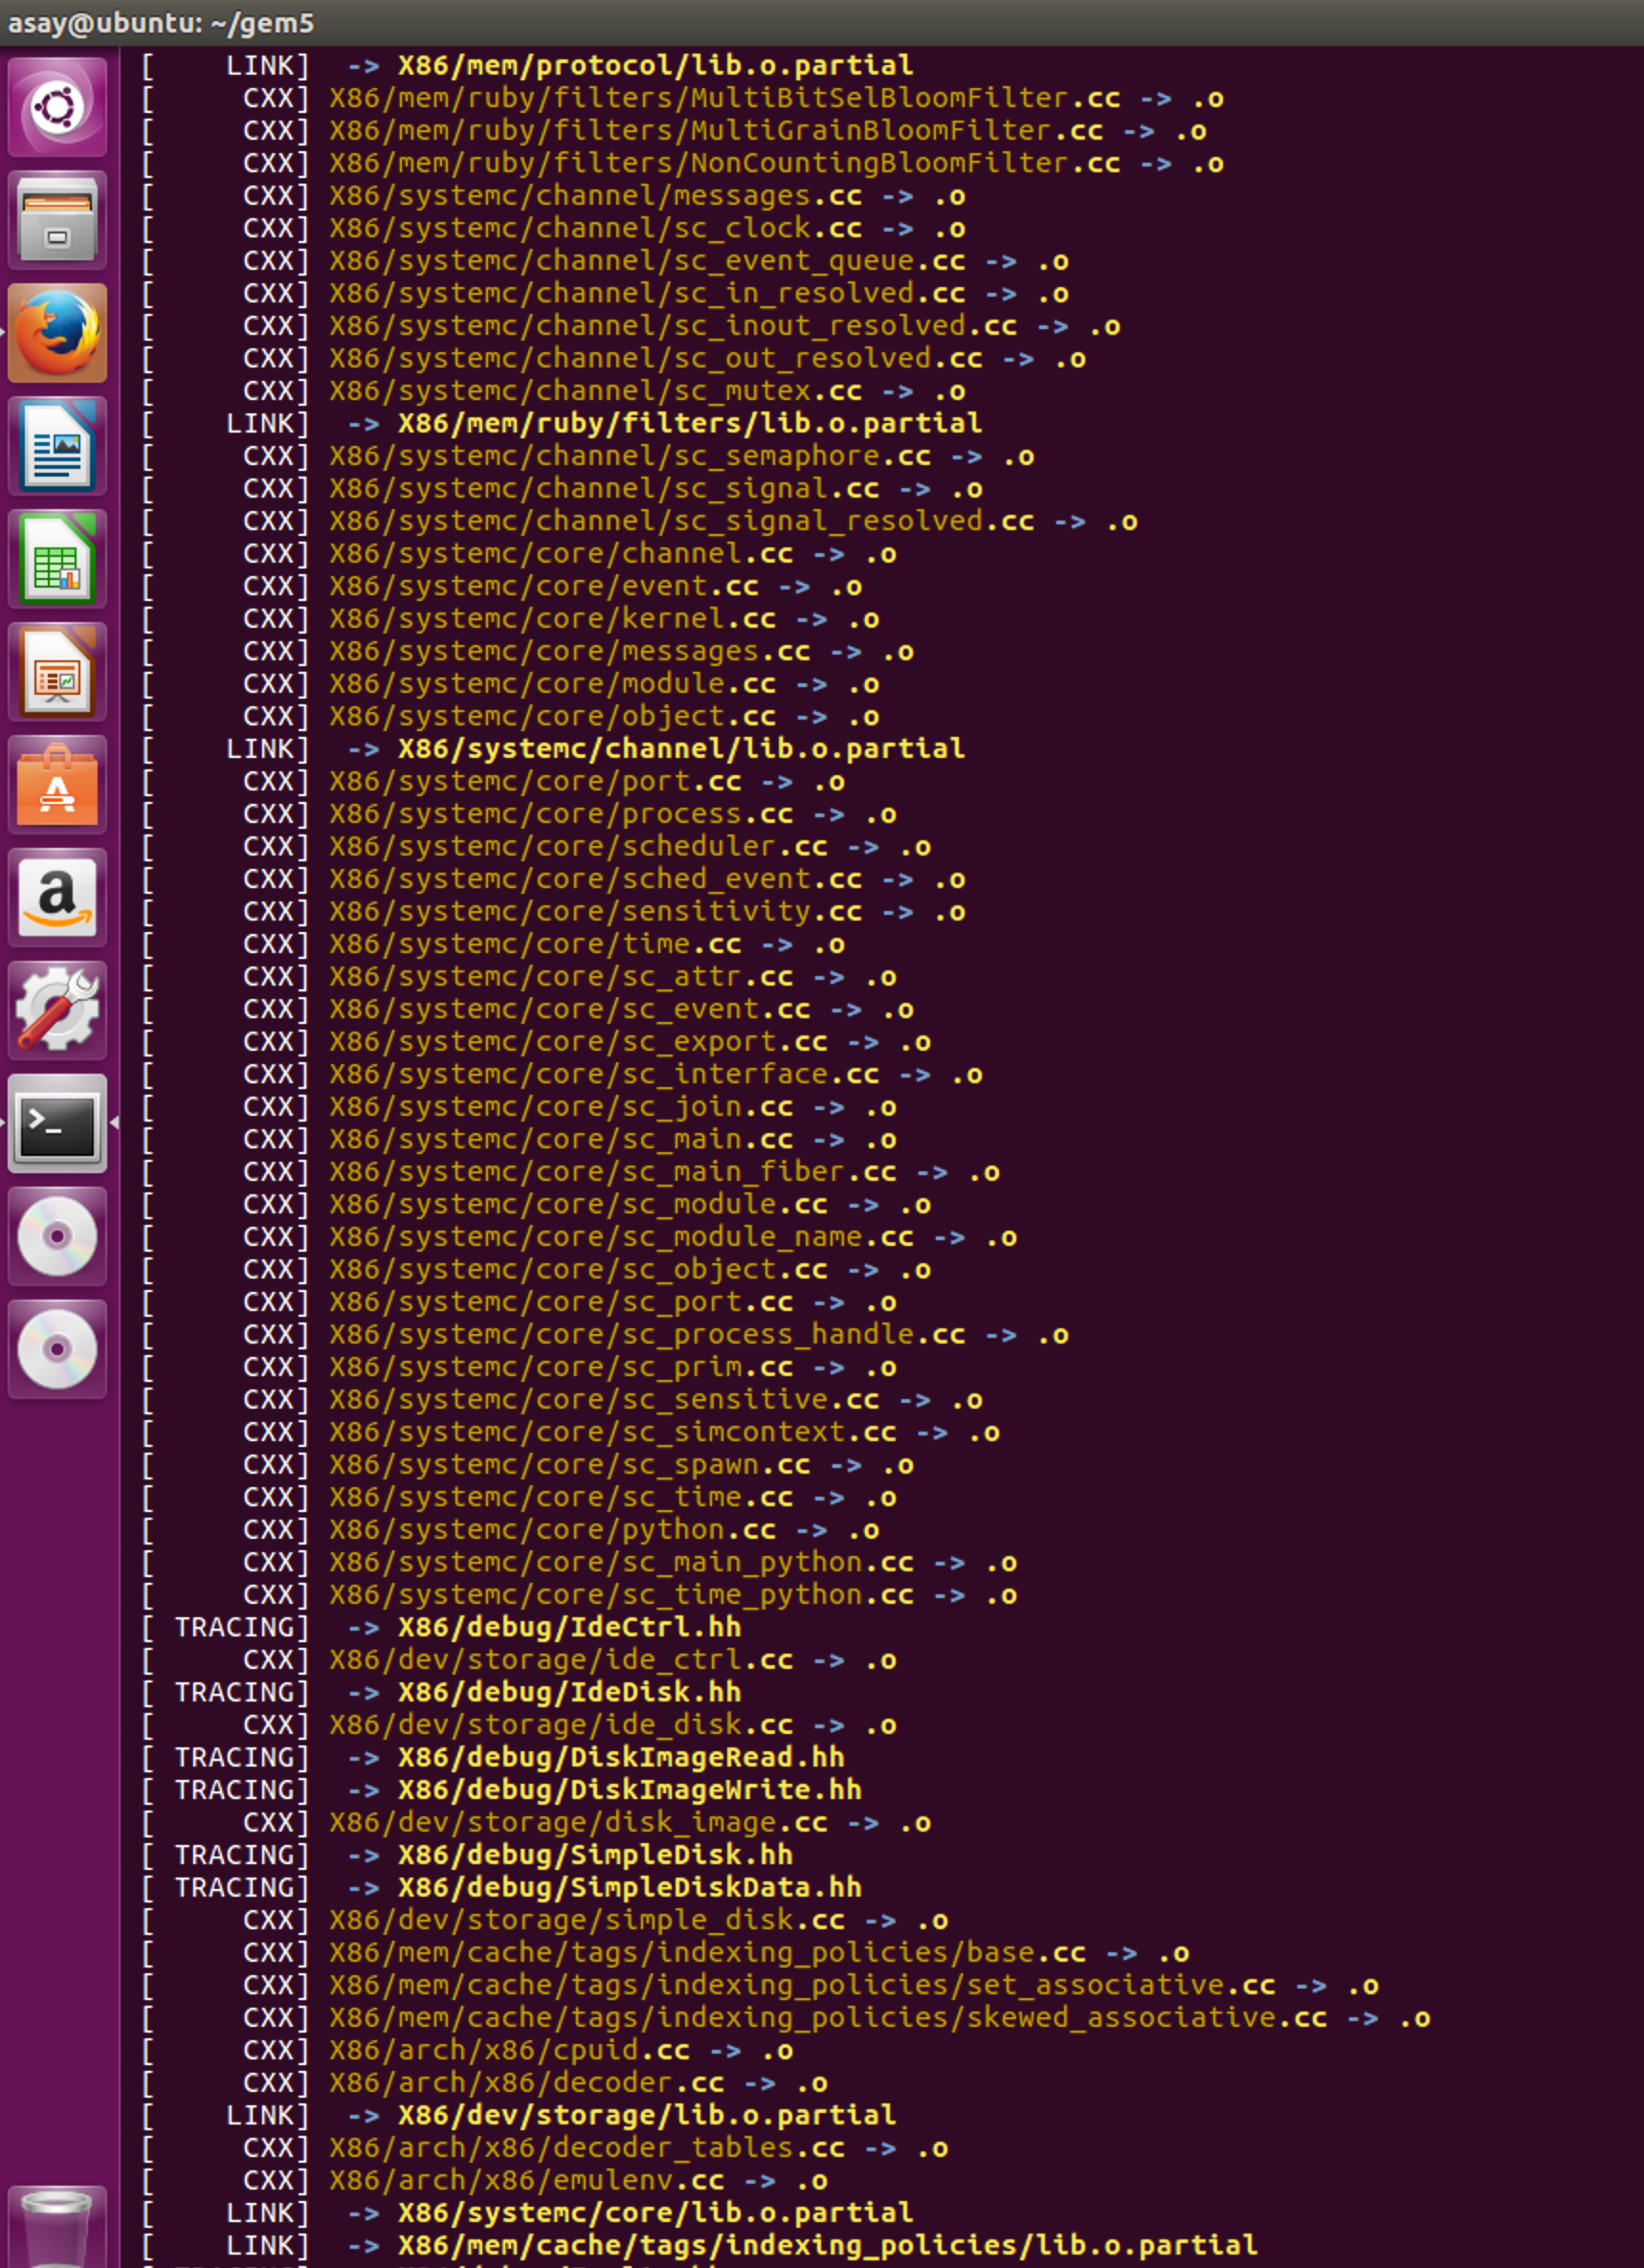
\includegraphics[width=1\textwidth]{build9}
%	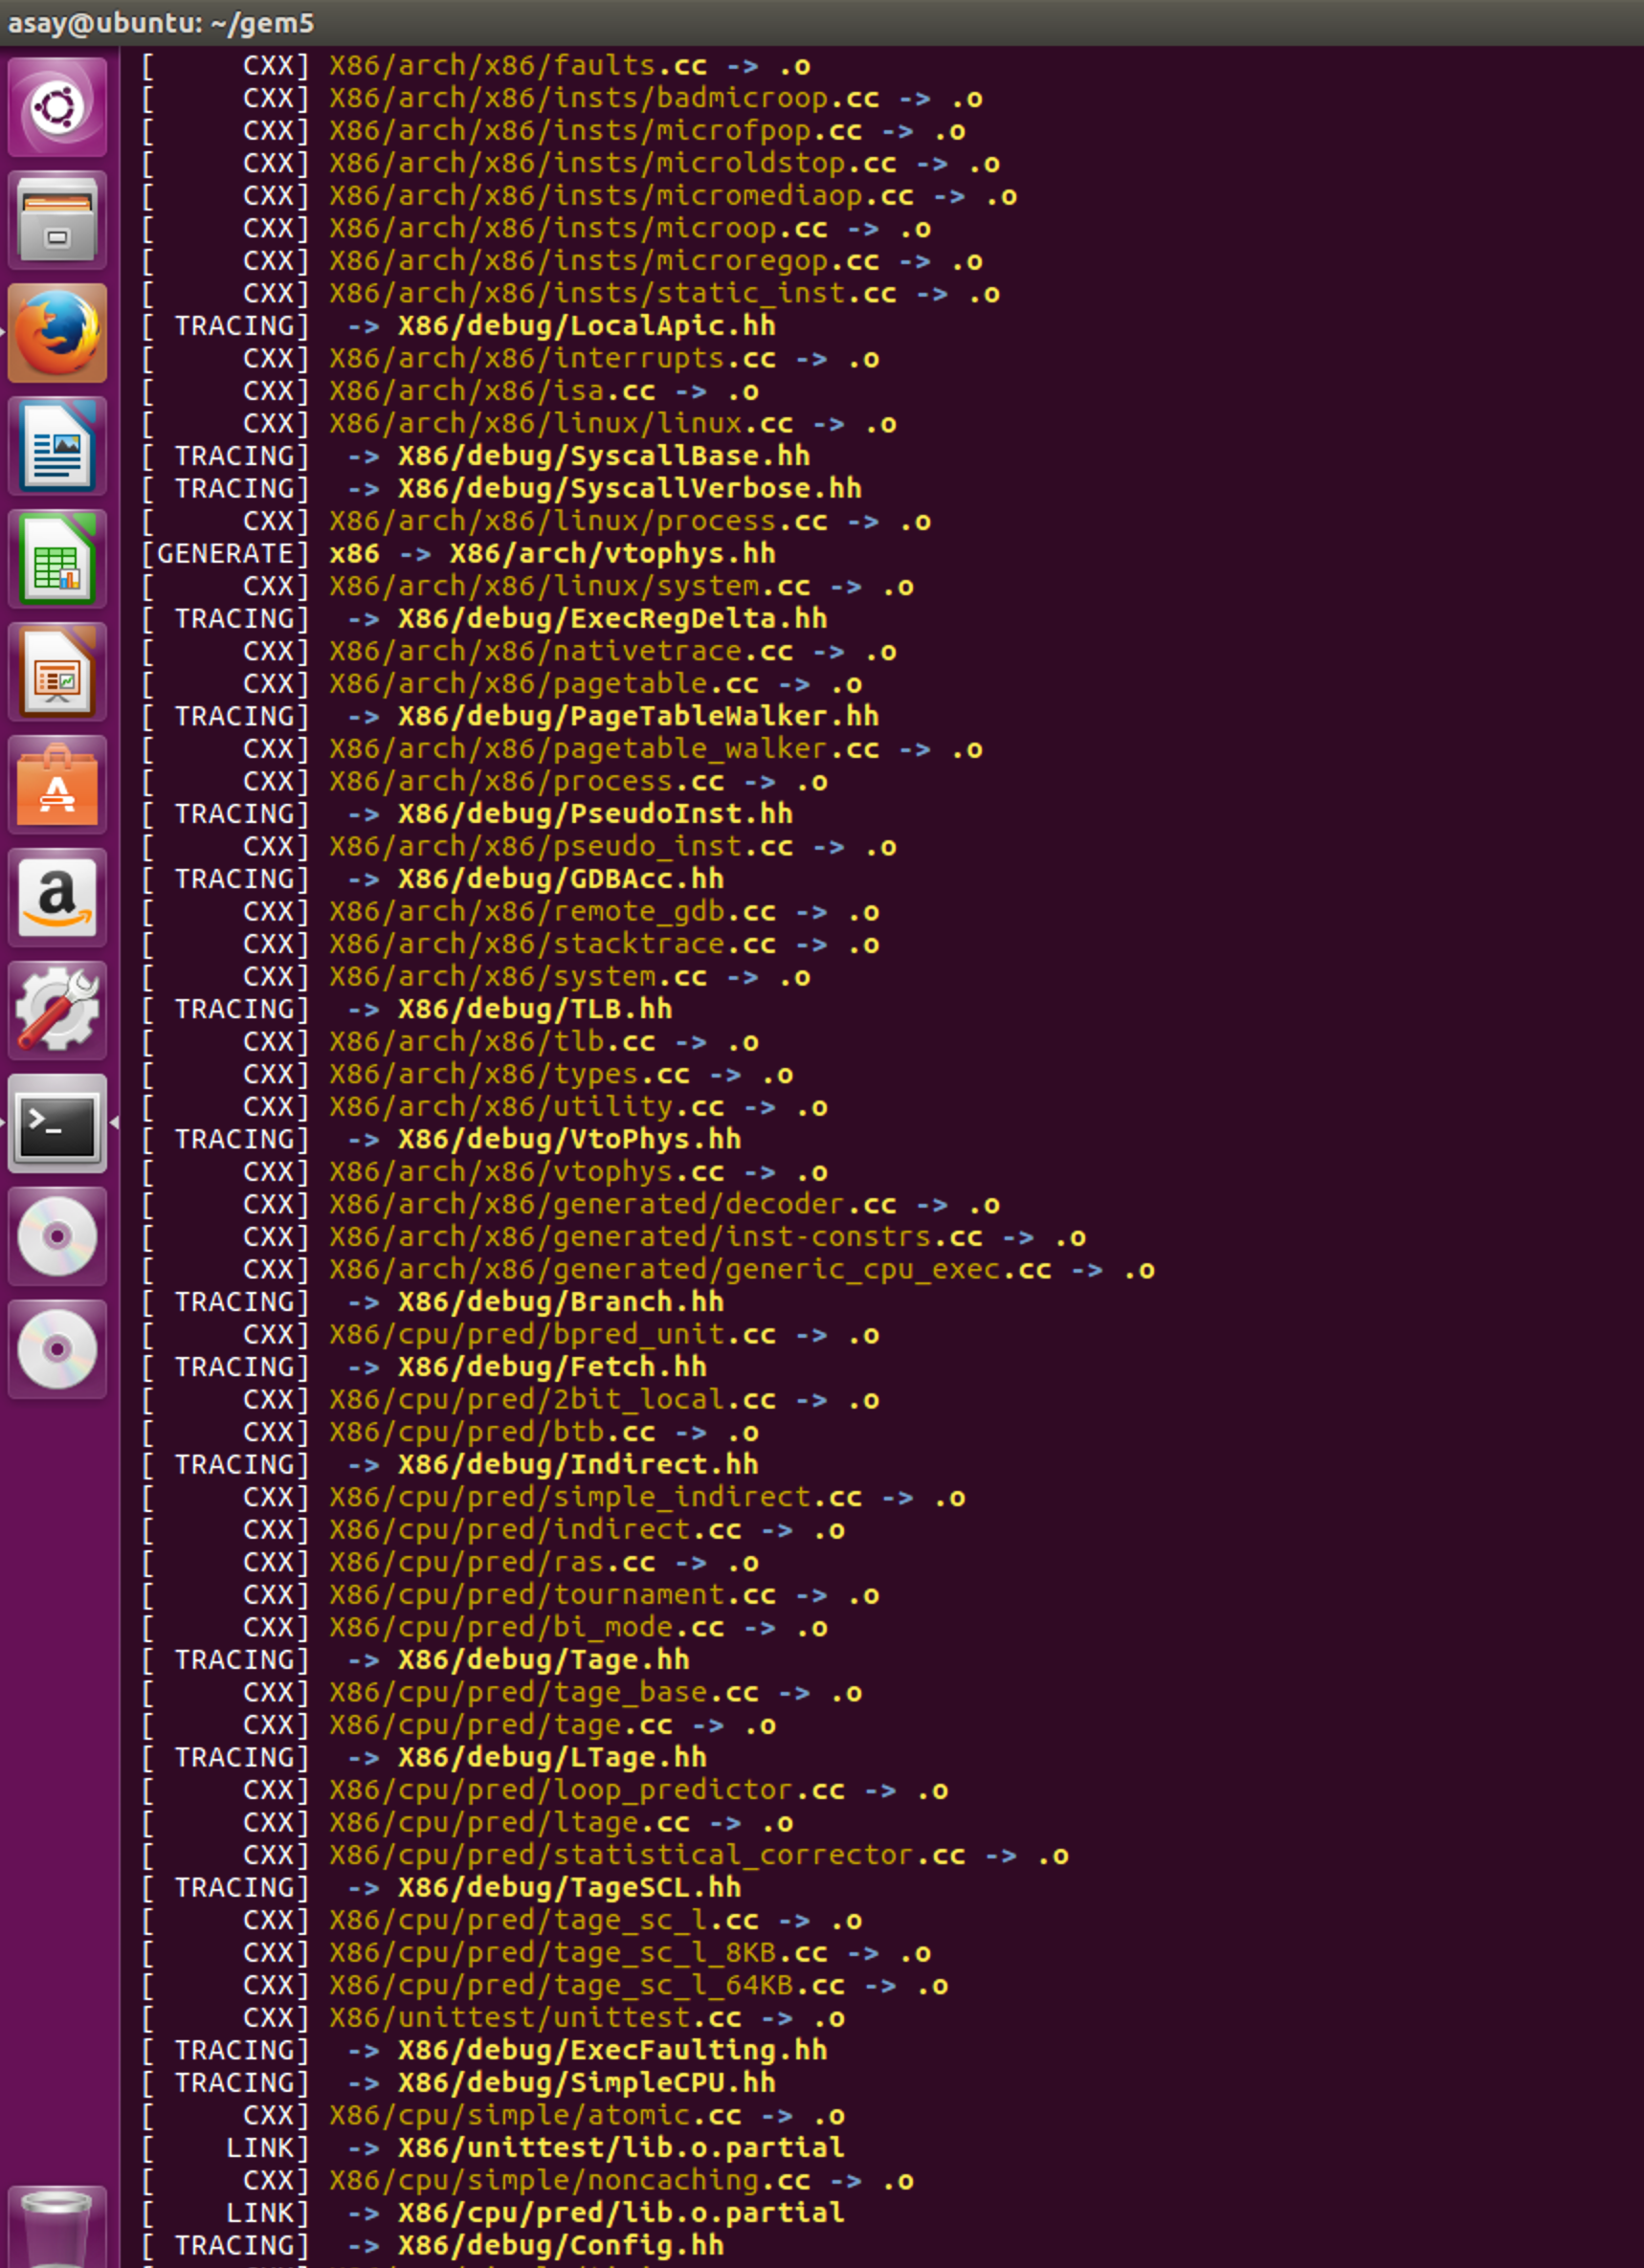
\includegraphics[width=1\textwidth]{build8}
%	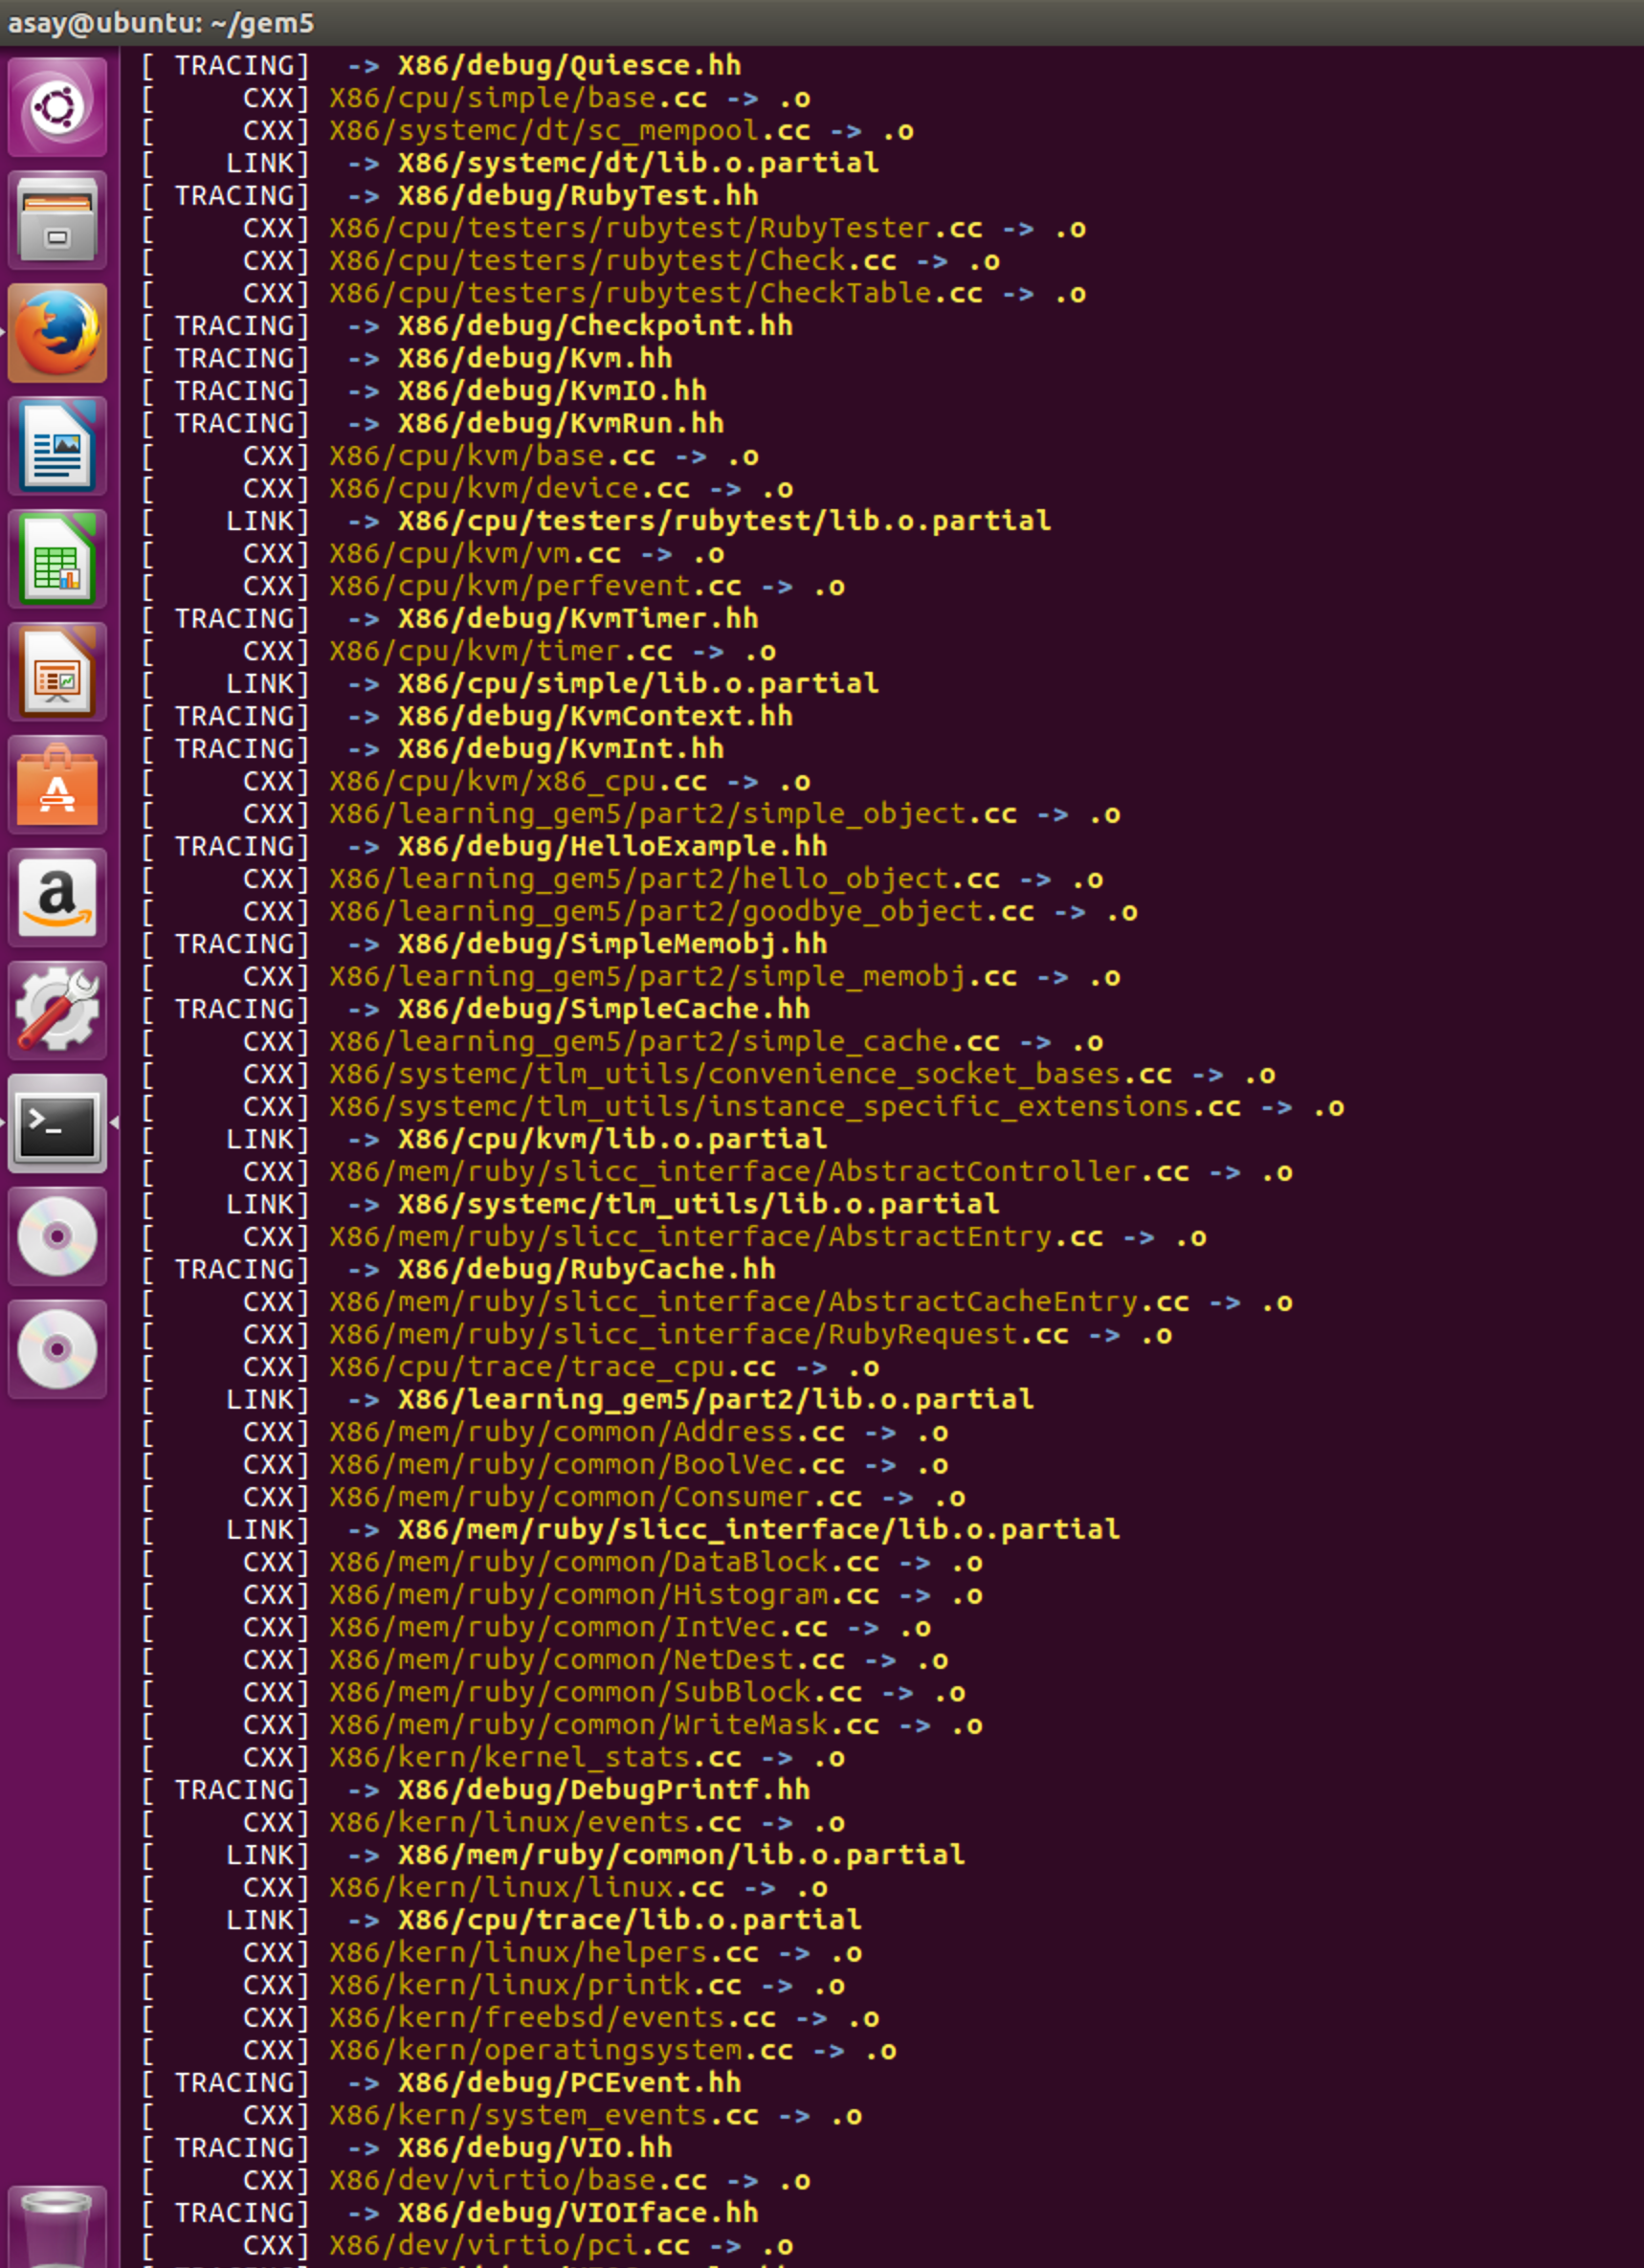
\includegraphics[width=1\textwidth]{build7}
%	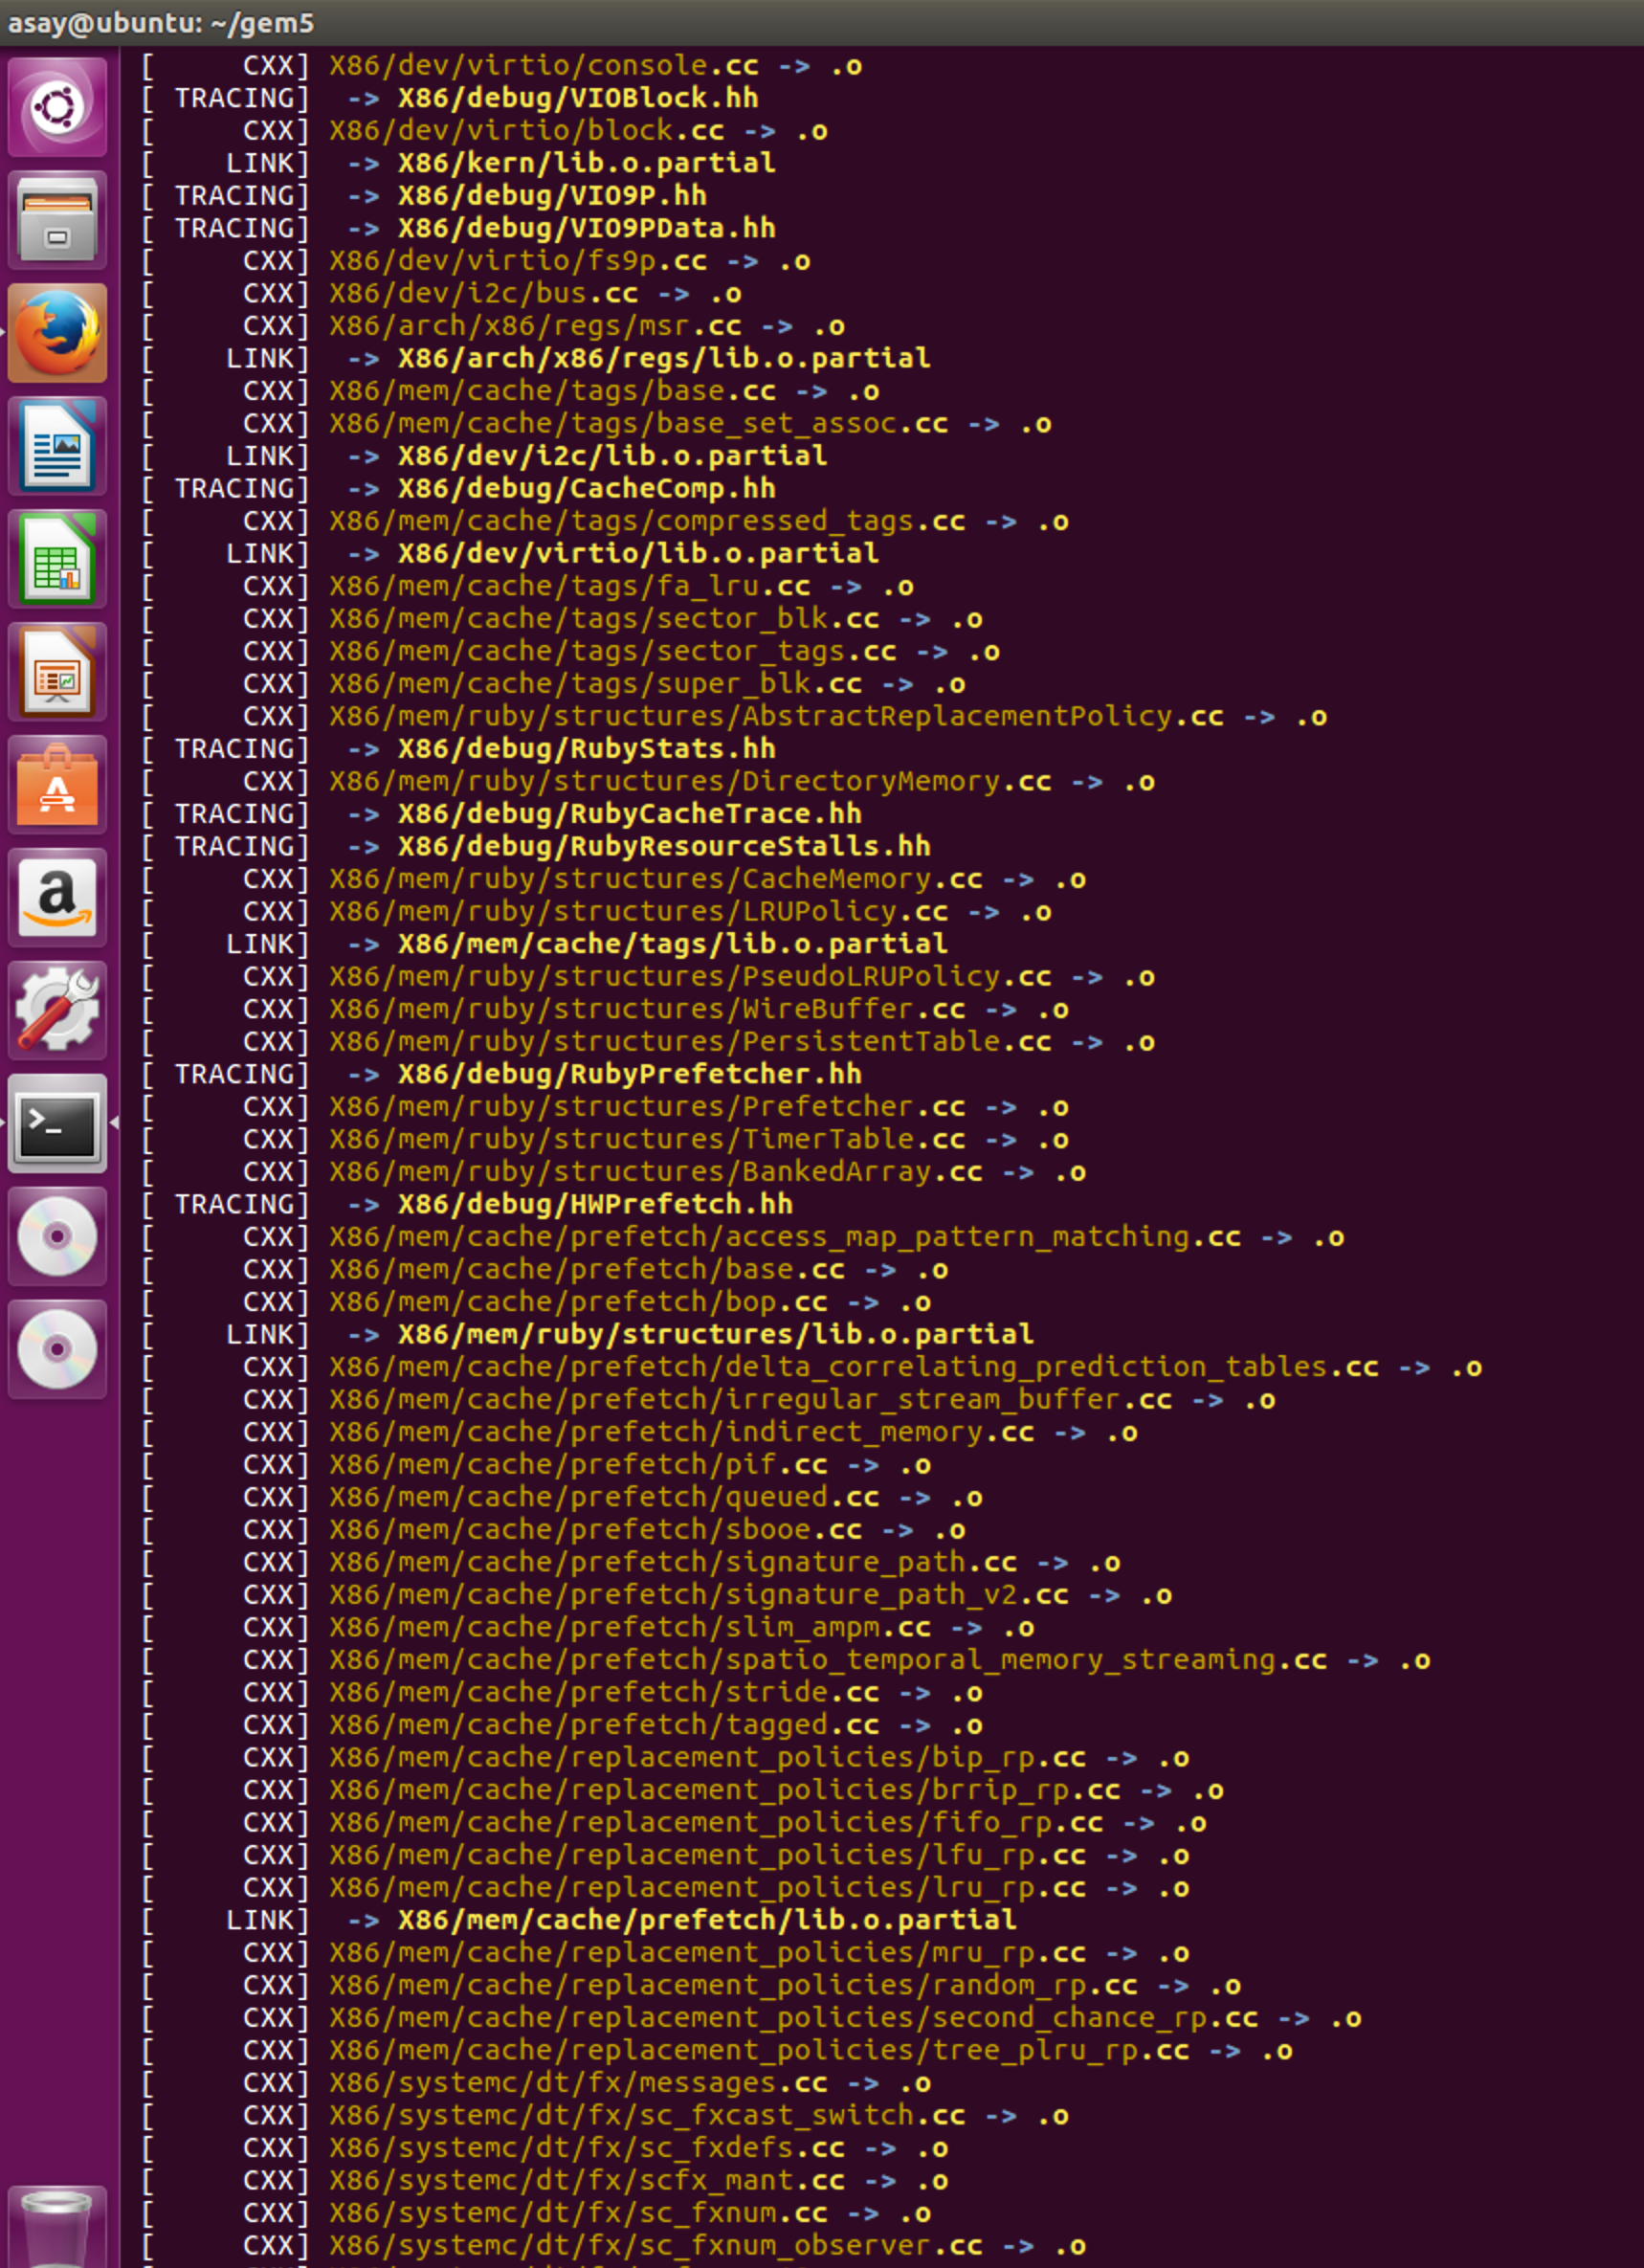
\includegraphics[width=1\textwidth]{build6}
%	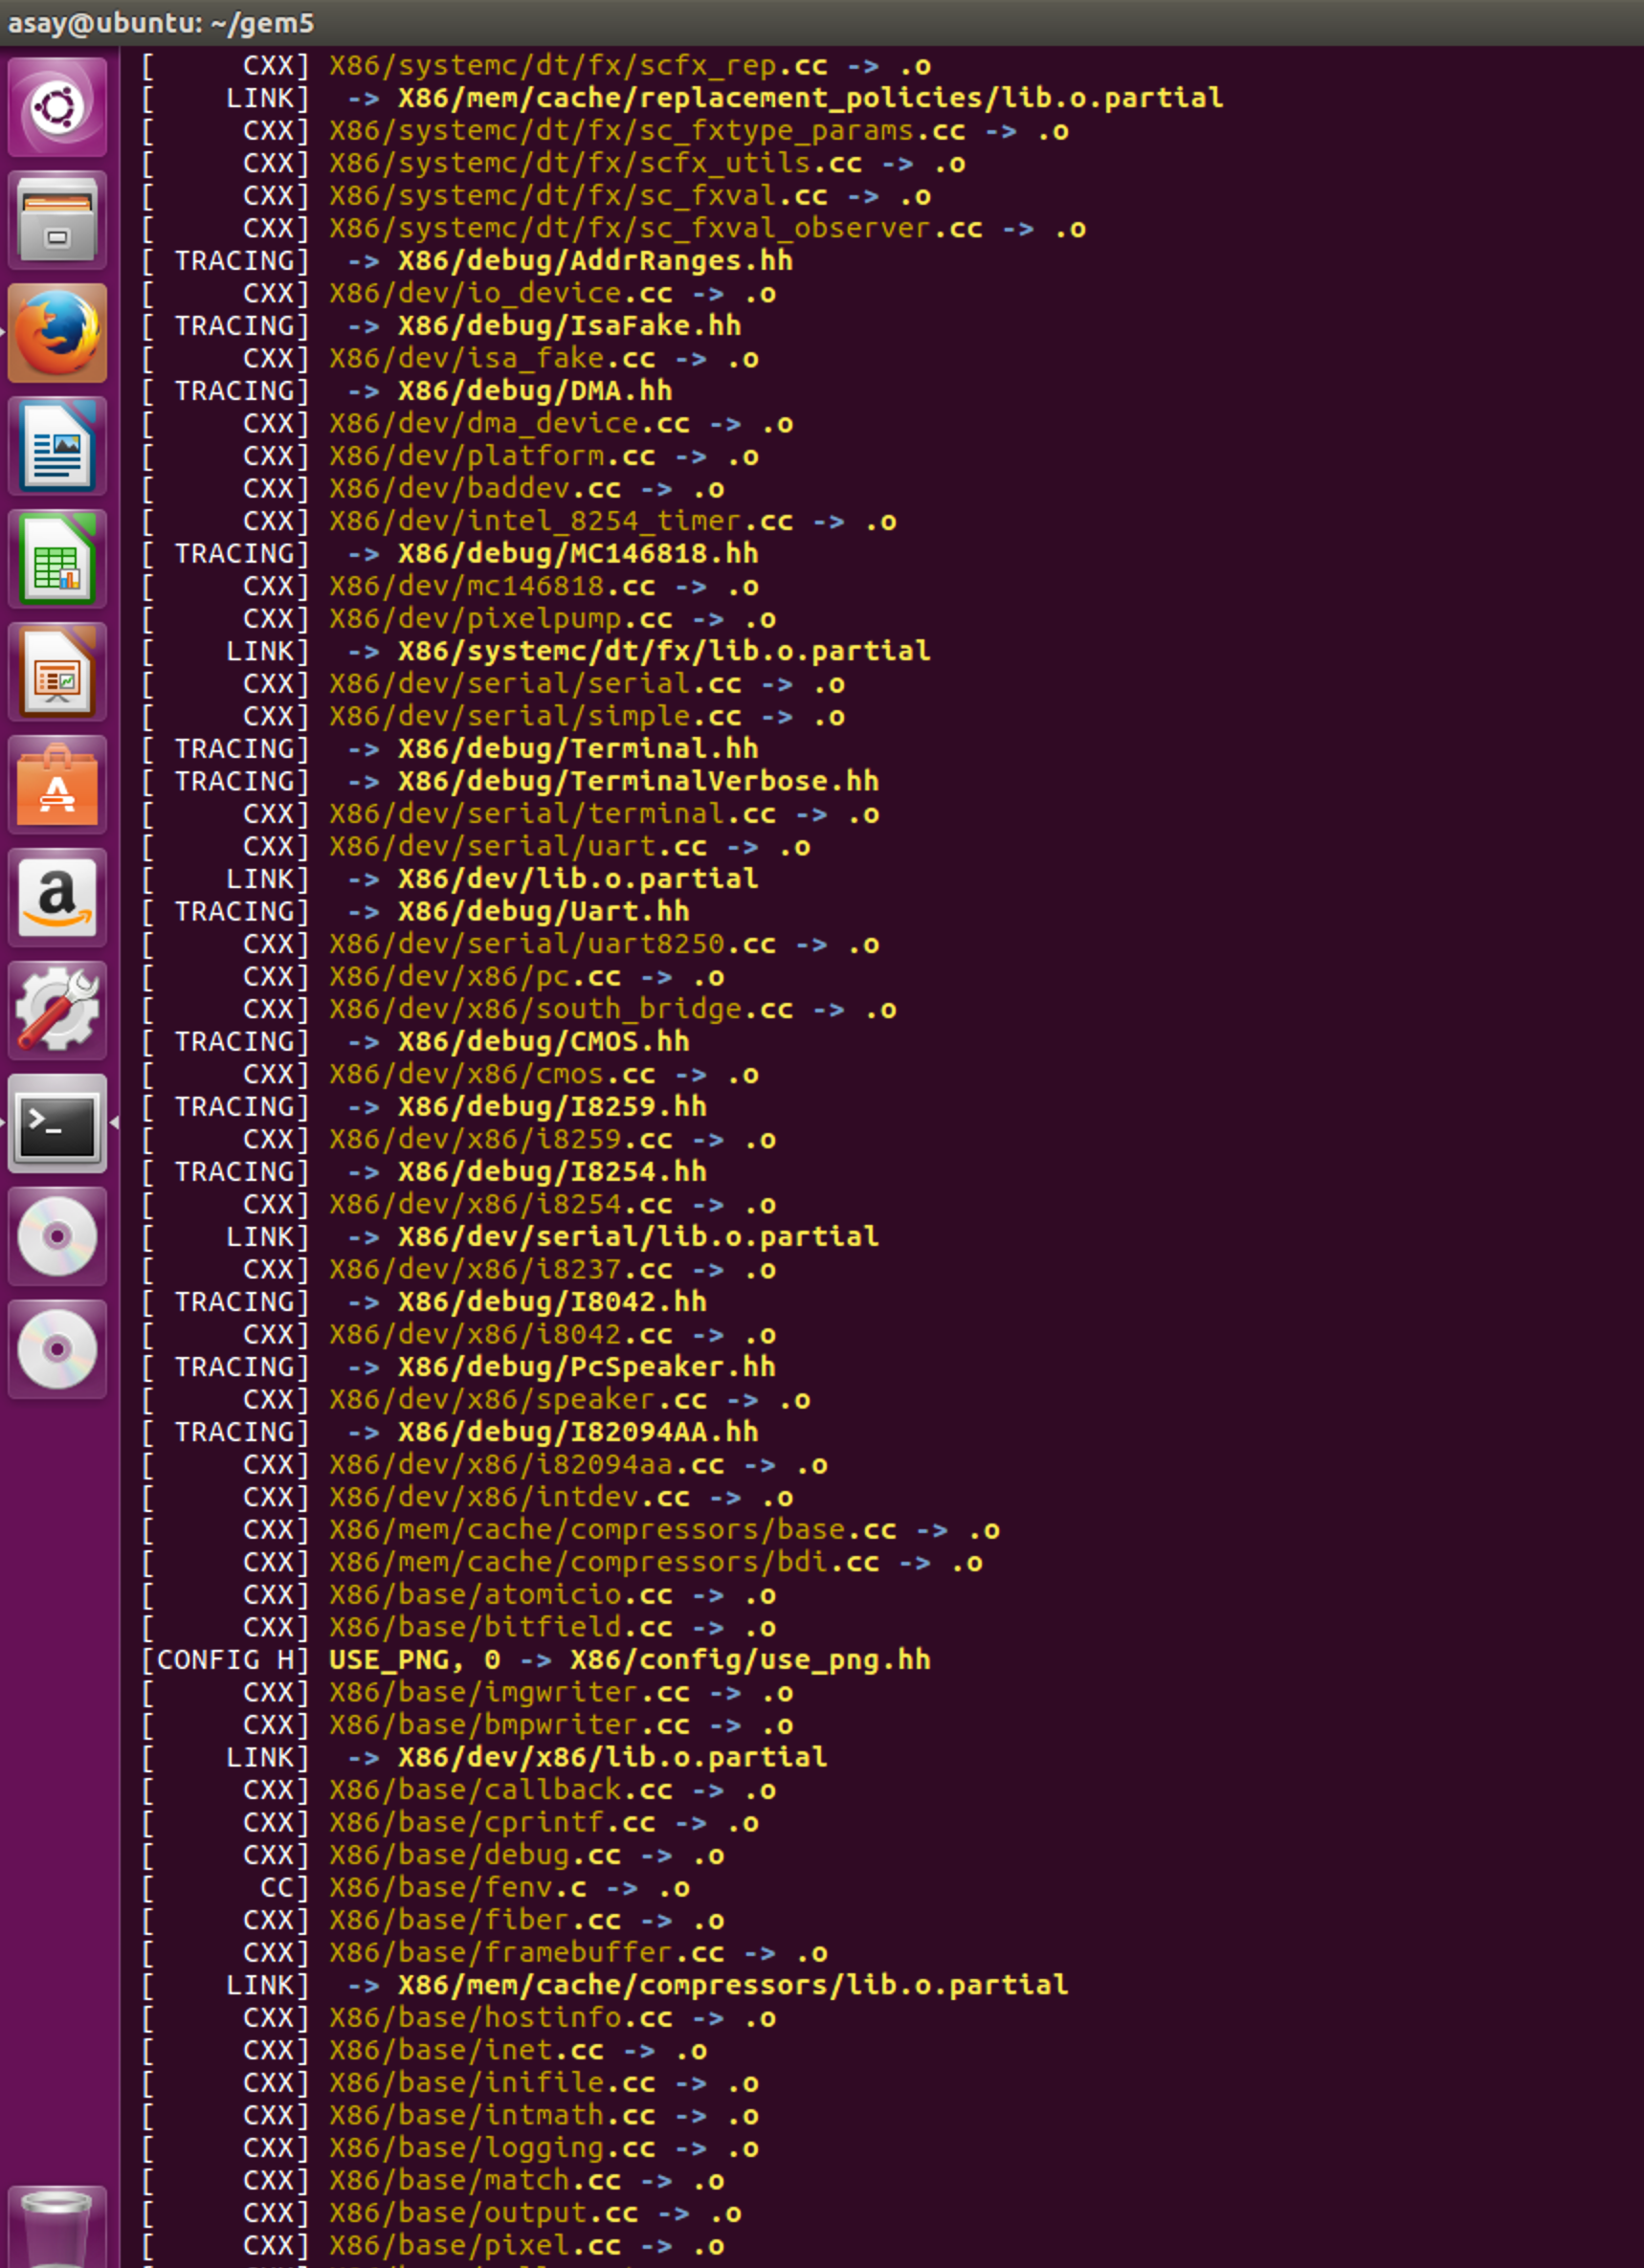
\includegraphics[width=1\textwidth]{build5}
%	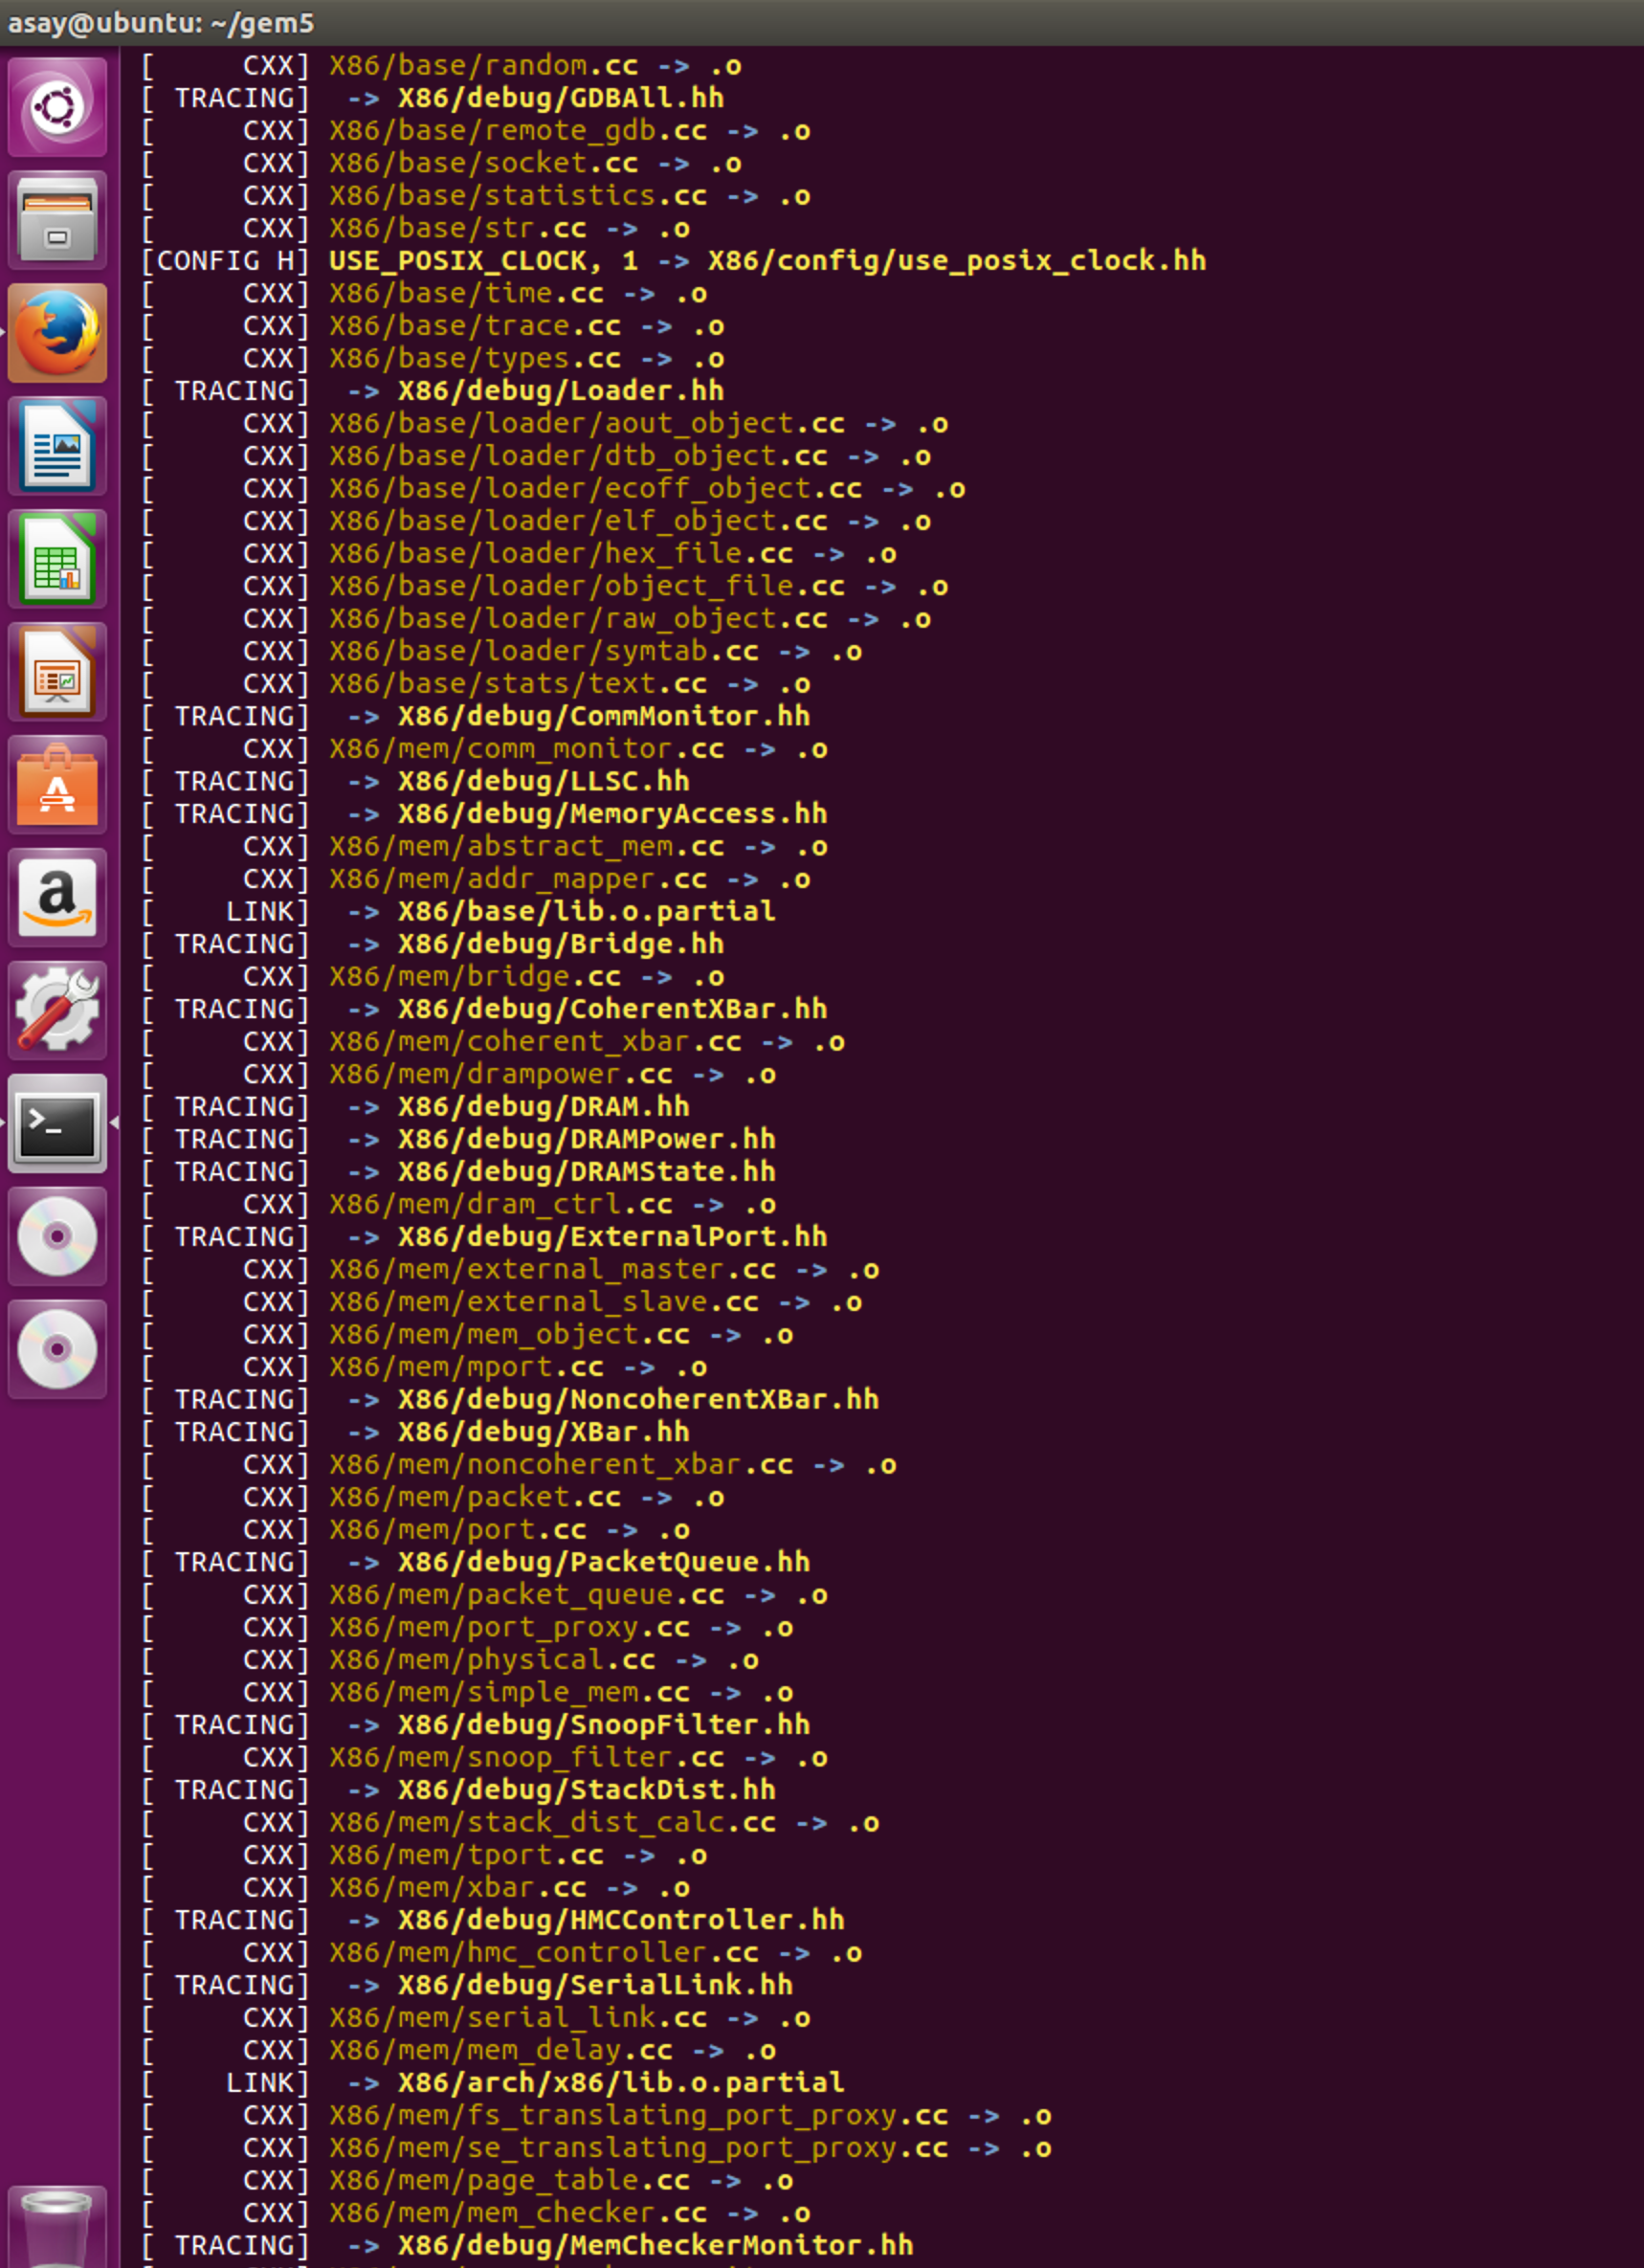
\includegraphics[width=1\textwidth]{build4}
%	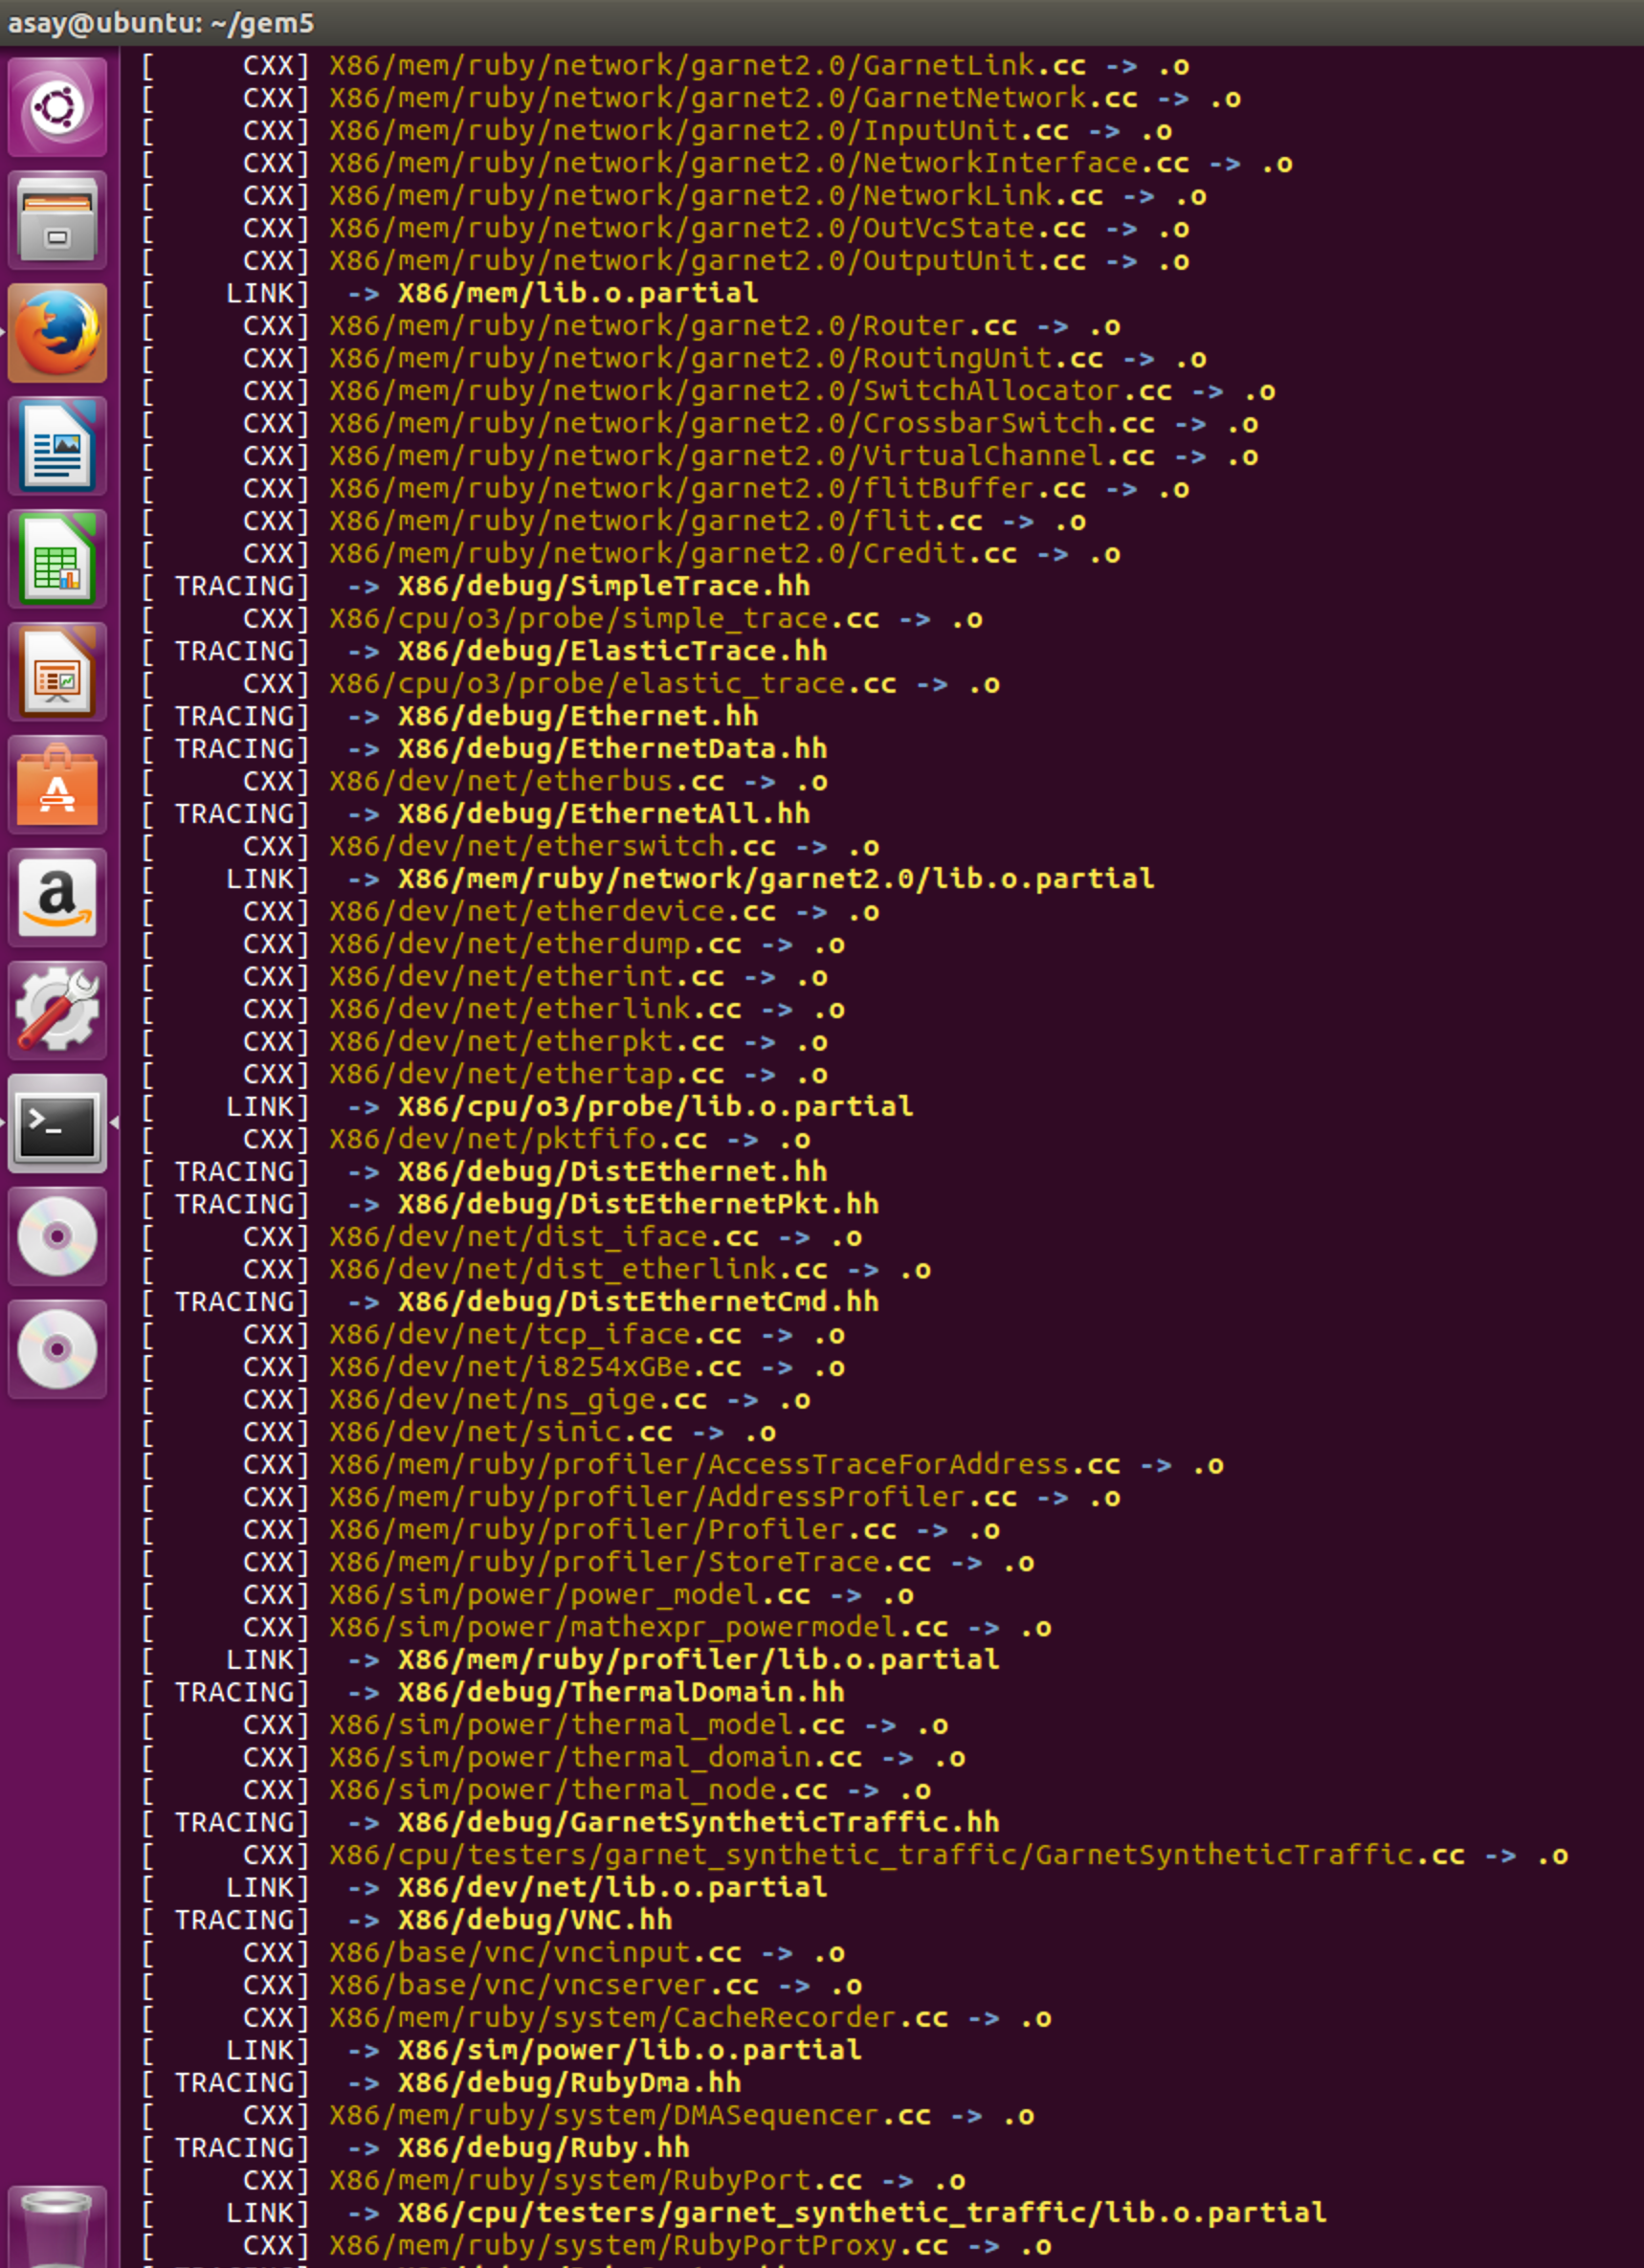
\includegraphics[width=1\textwidth]{build3}
	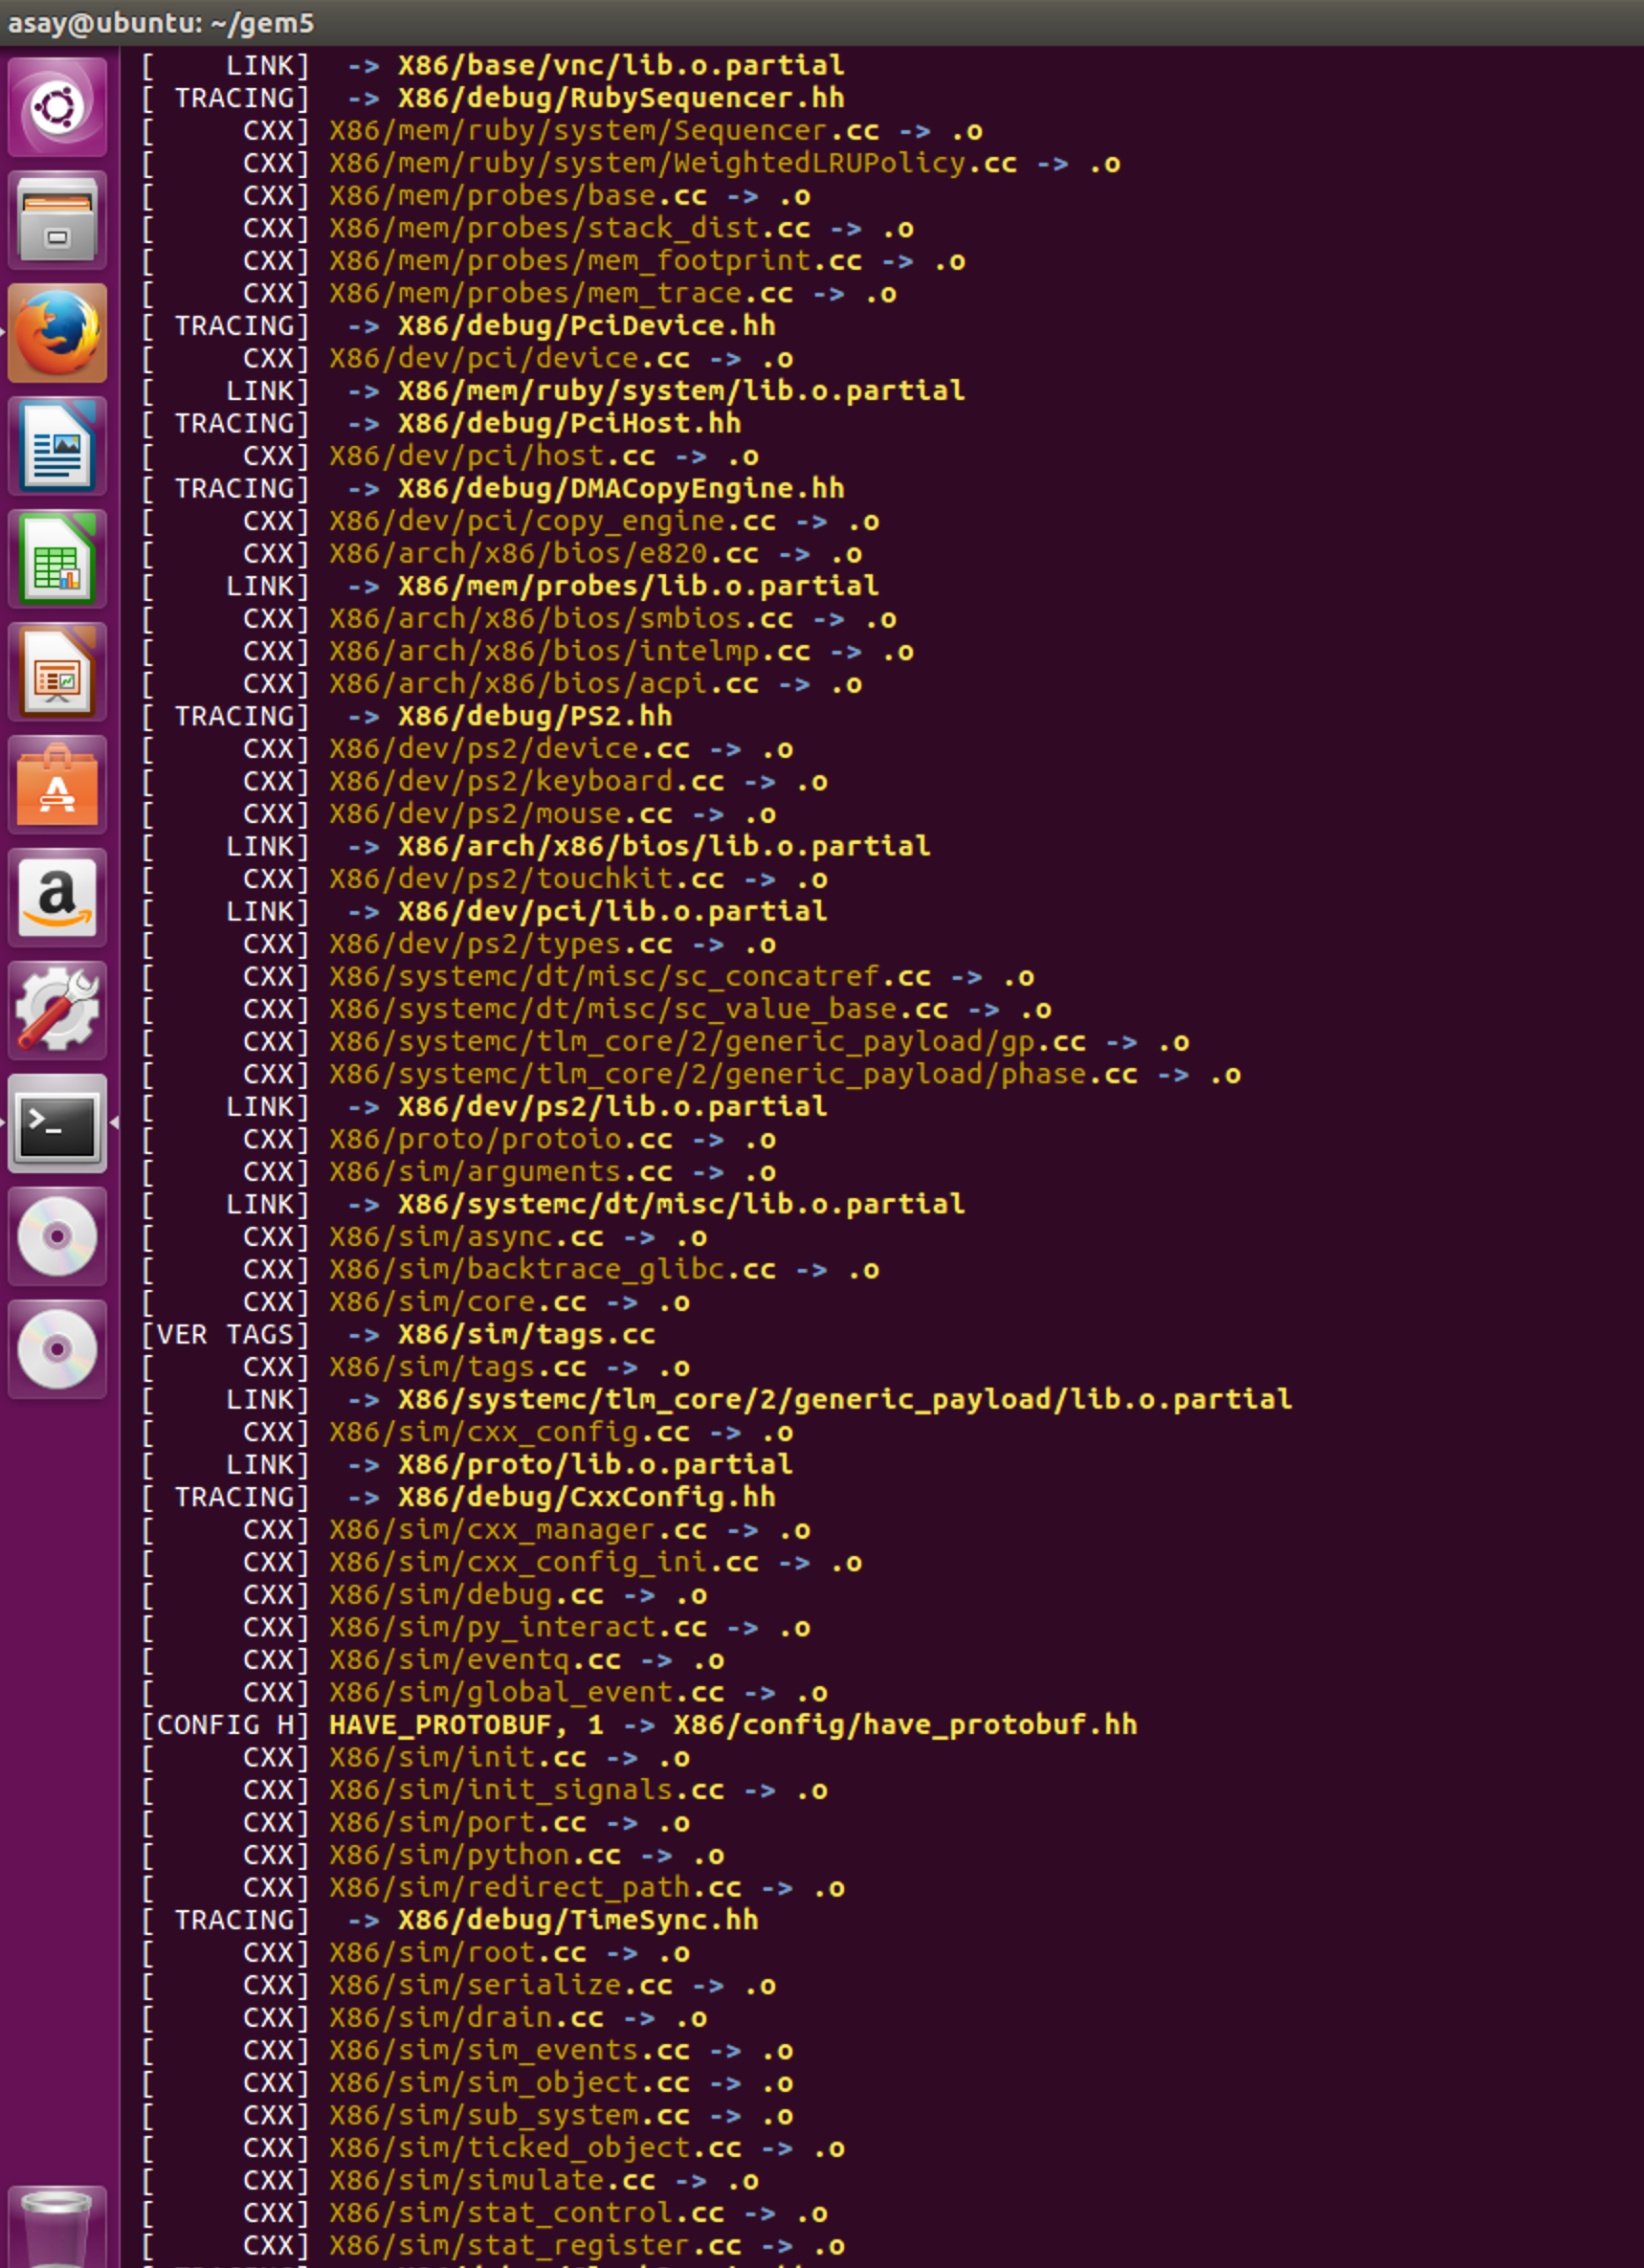
\includegraphics[width=1\textwidth]{build2}
	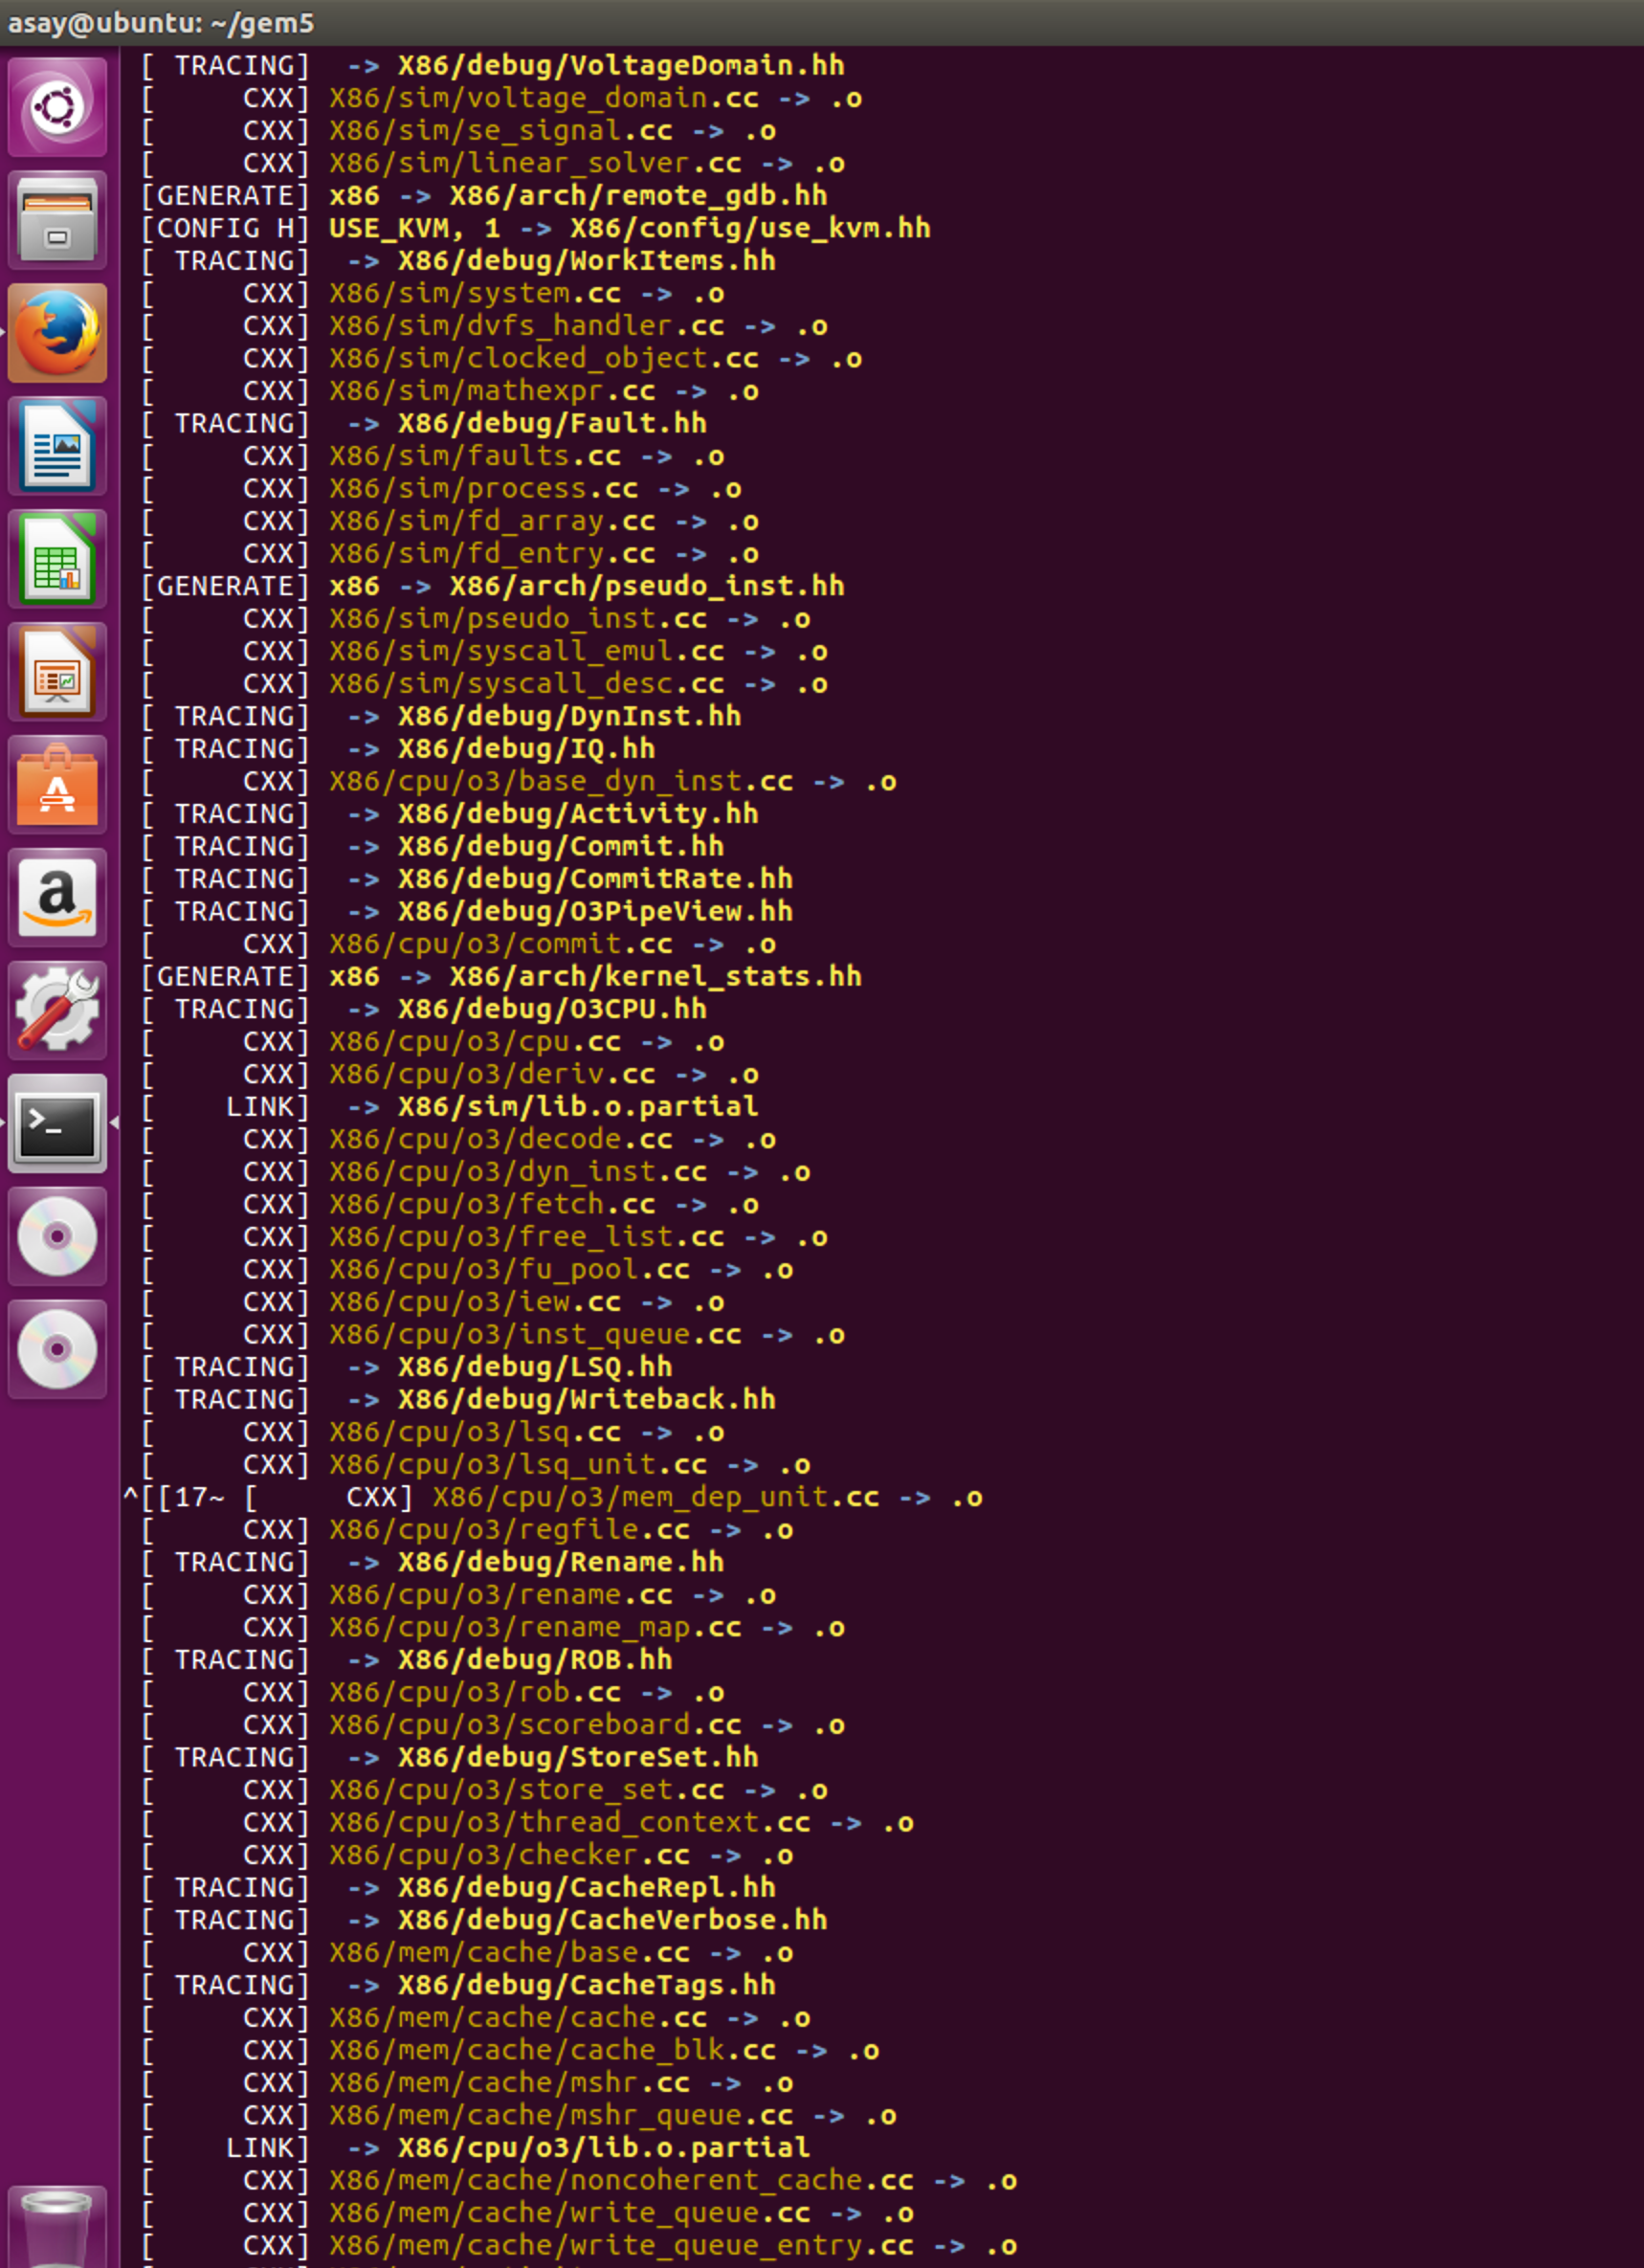
\includegraphics[width=1\textwidth]{build1}
	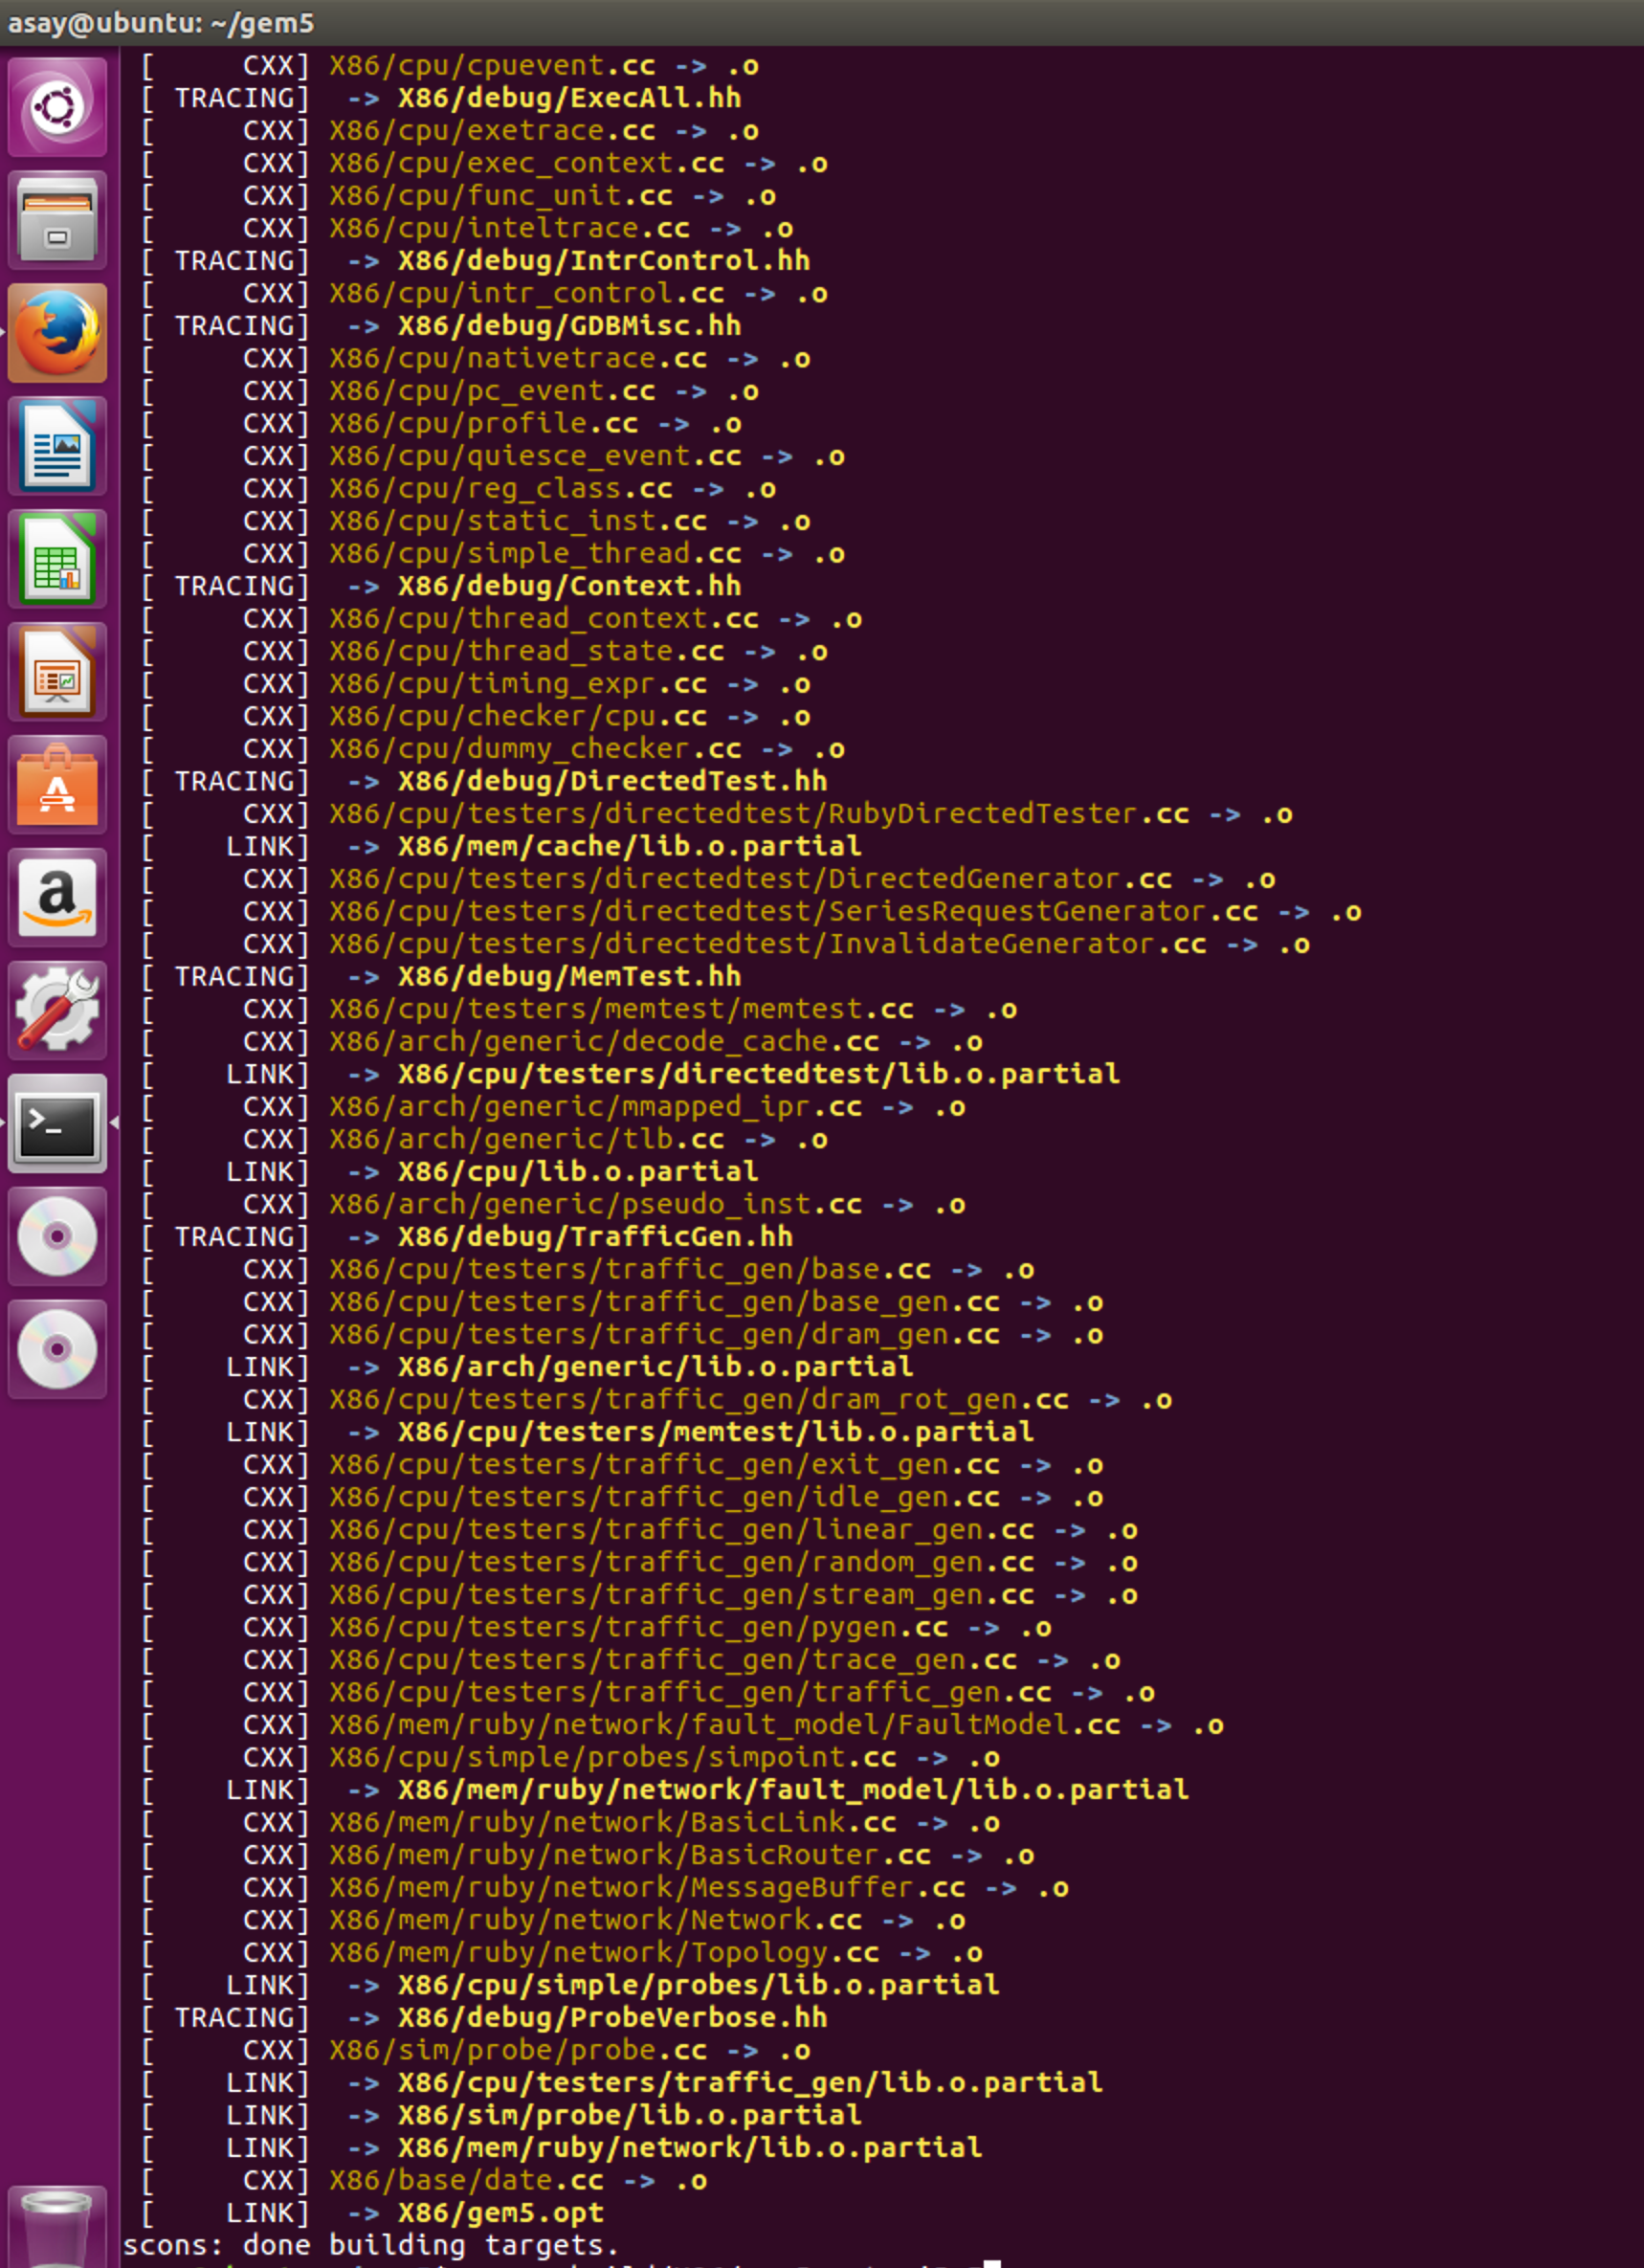
\includegraphics[width=1\textwidth]{finalbuild}
\end{center}
\newpage
\section*{اجرای یک برنامه دلخواه }
برای این بخش یک برنامه دو عدد را جمع می زند در نظر گرفته شده که فایل برنامه به پیوست ارسال می شود  . \\
ابتدا یک فایل به نام 
\textcolor{red}{\lr{mytest}}
داخل فایل 
\lr{gem5}
به وجود می آوریم با دستور 
\begin{center}
	\lr{mkdi mytest}
\end{center}
حال داخل فایل ساخته شده کد پیوست شده را داخل آن قرار می دهیم و بعد یک فایل اجرایی از آن می گیریم . 
\begin{center}
	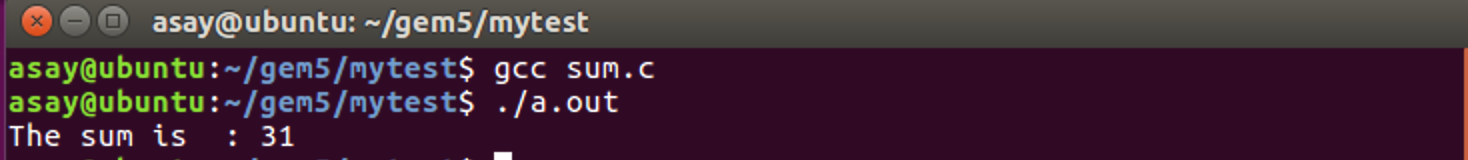
\includegraphics[width=1\textwidth]{sumbuild}
\end{center}
حال فایل 
\lr{sum.c}
را بر روی معماری 
\lr{x86}
با دستور زیر اجرا می کنیم  : 
\begin{center}
	\lr{./build/X86/gem5.opt configs/example/se.py -c mytest/a.out
}
\end{center}
که نتیجه آن به شرح زیر می باشد : 
\begin{center}
		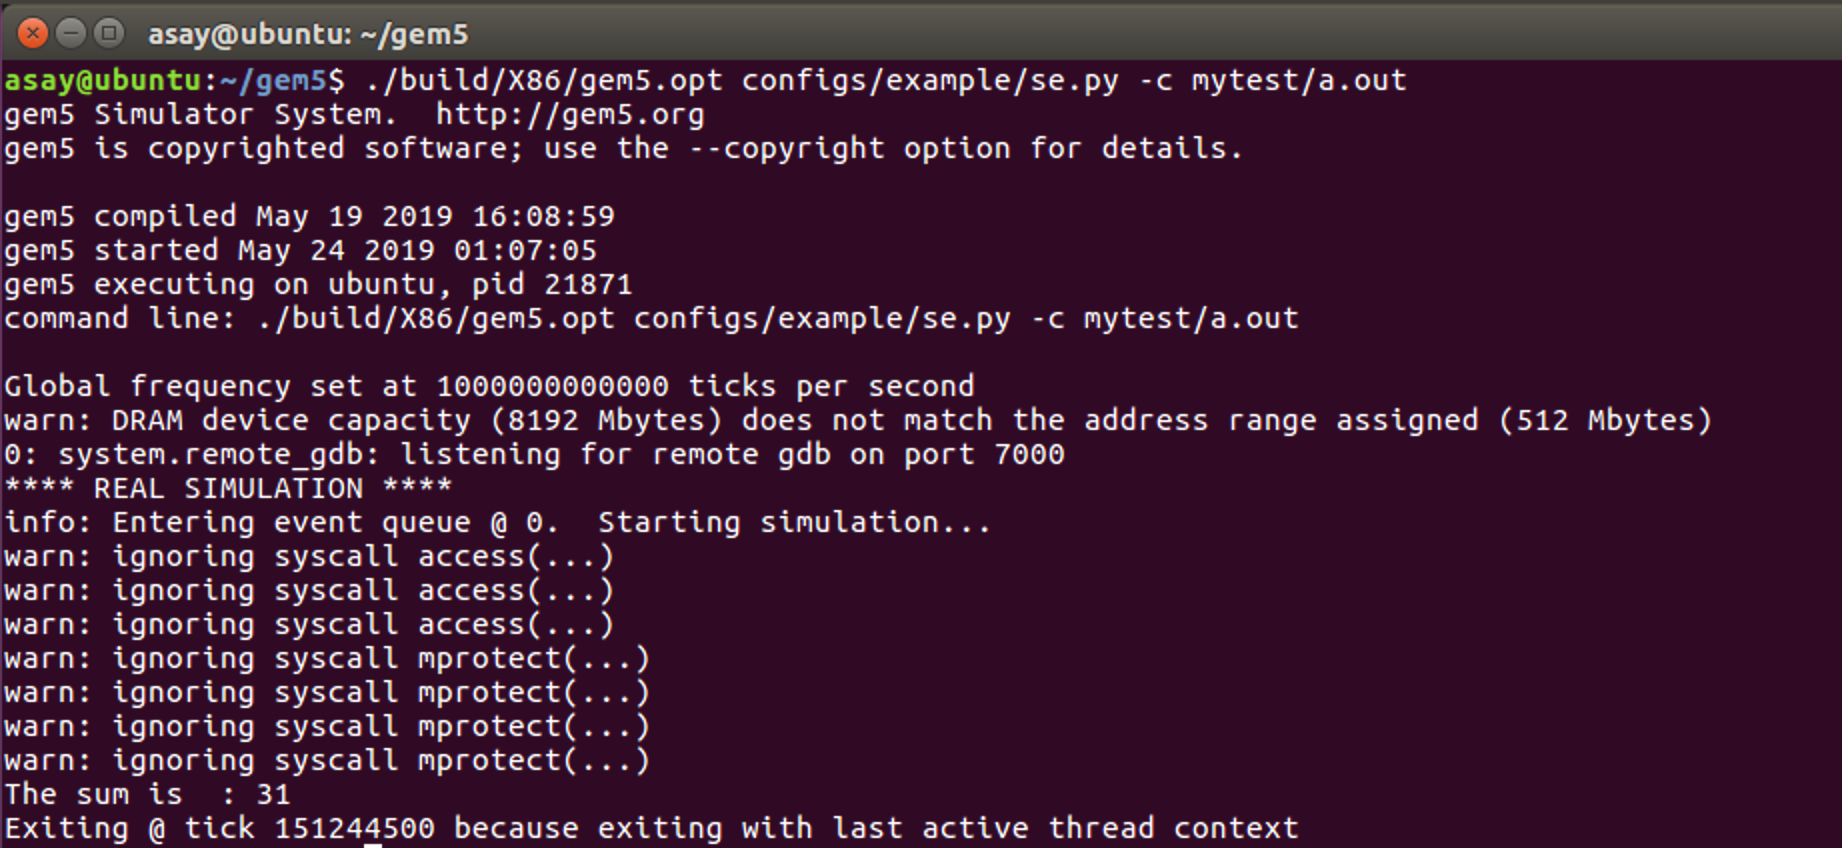
\includegraphics[width=1\textwidth]{sumonx86}
\end{center}
که فایل 
\lr{stat.txt }
به پیوست ارسال شده است  . 
\newpage
\section*{اجرا با 
	\lr{cacheline}
	ها و 
	\lr{cachesize}
	های متفاوت }
\subsection*{\lr{Cachesize = 1kb , cacheline : 16}}
\begin{center}
	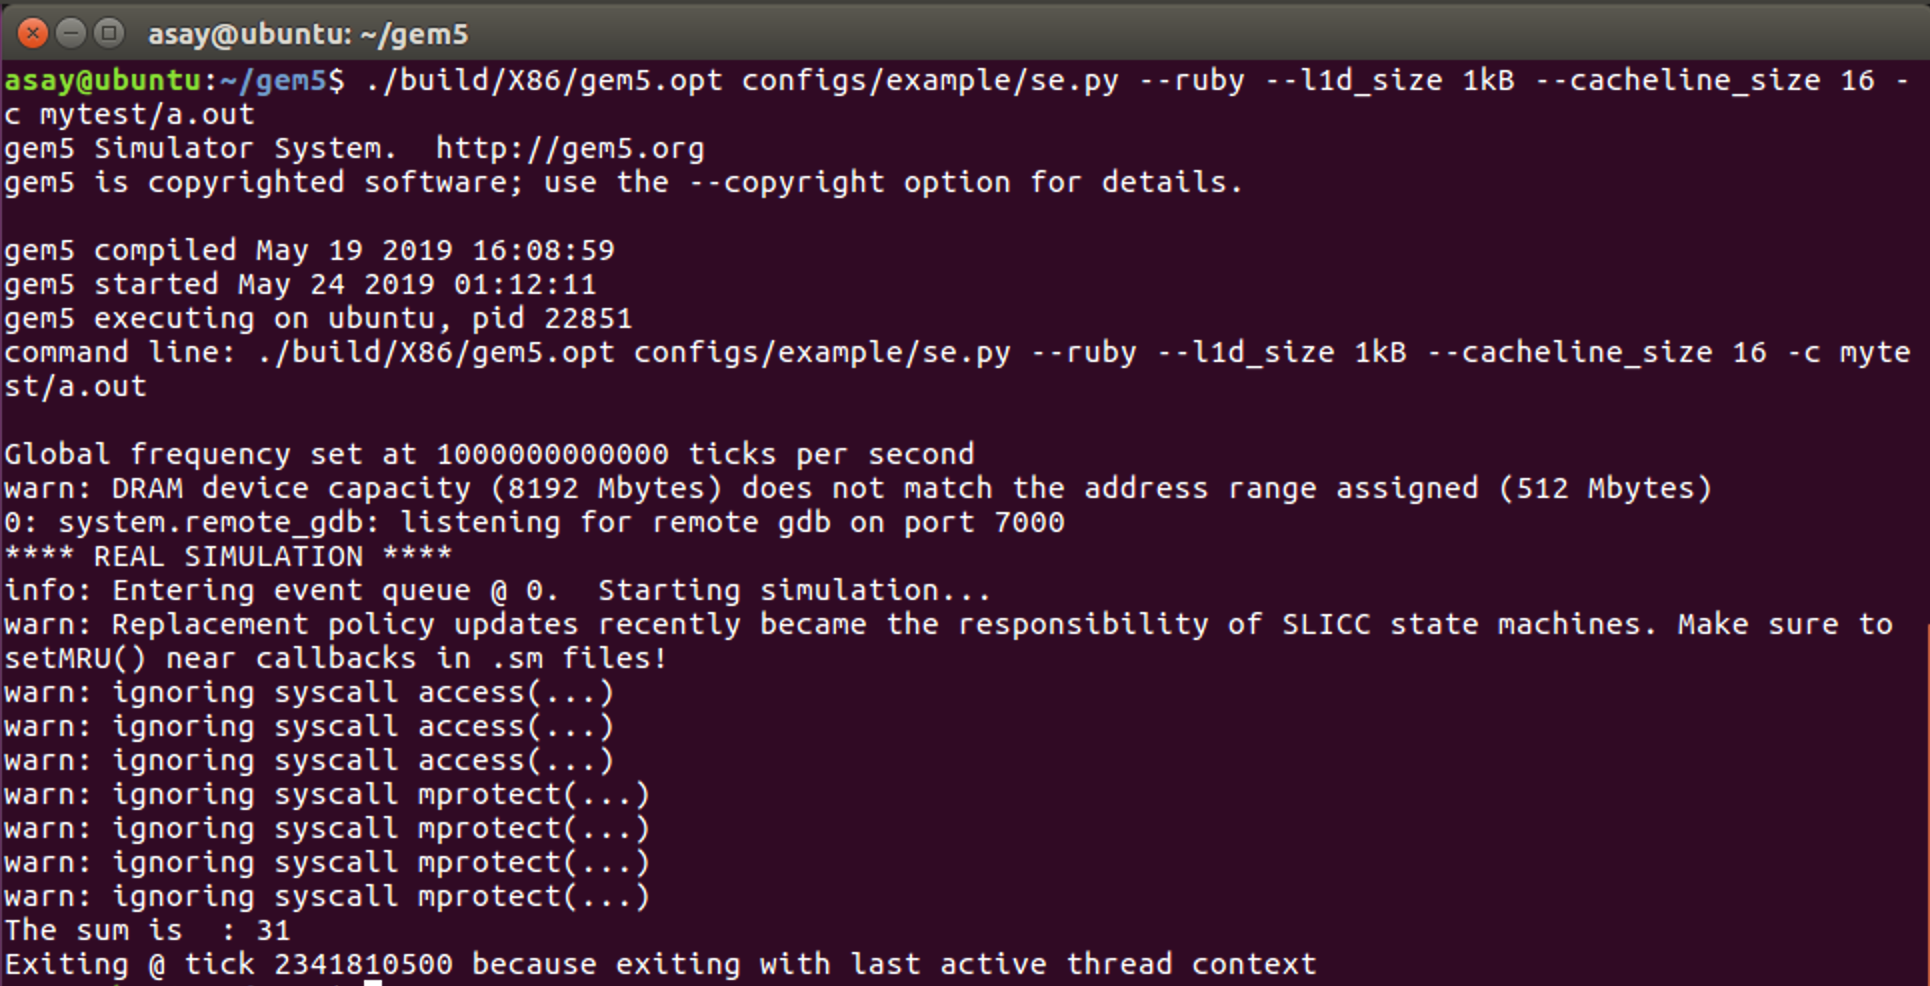
\includegraphics[width=1\textwidth]{cacheline16}
\end{center}
\subsection*{\lr{Cachesize = 1kb , cacheline : 32}}
\begin{center}
	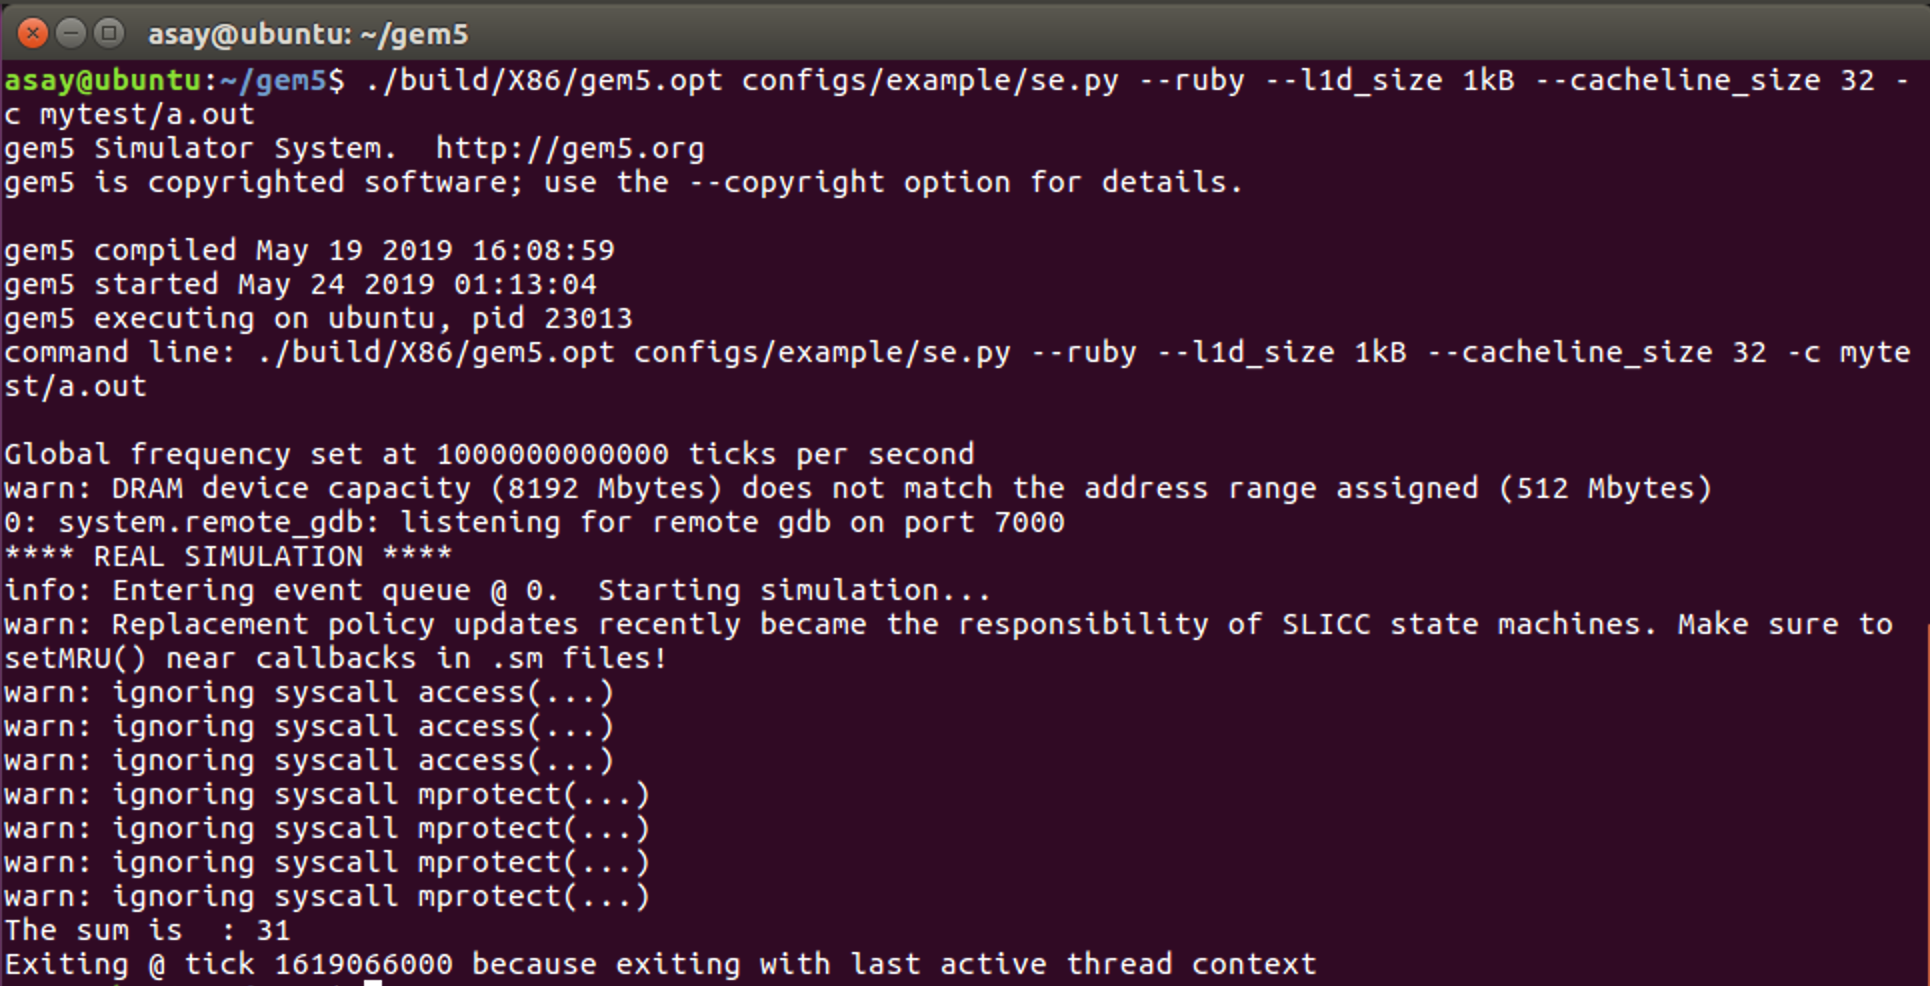
\includegraphics[width=1\textwidth]{cacheline32}
\end{center}
\subsection*{\lr{Cachesize = 1kb , cacheline : 64}}
\begin{center}
	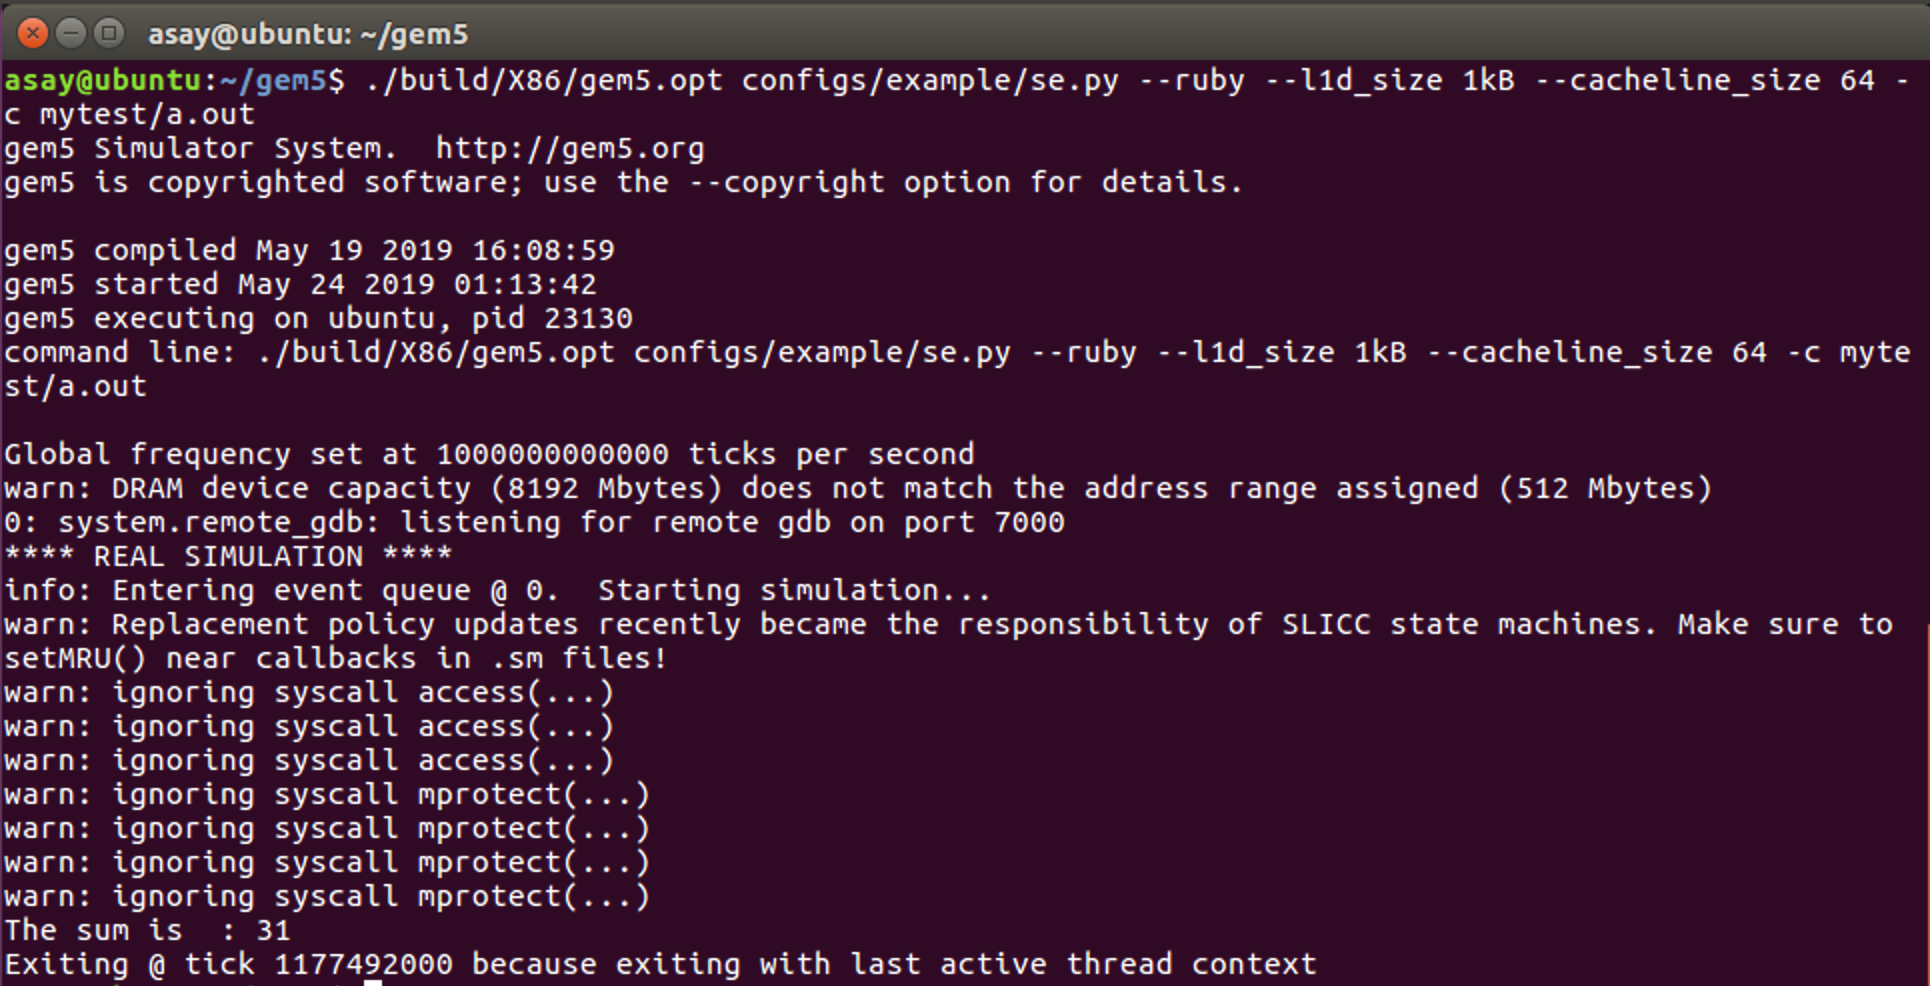
\includegraphics[width=1\textwidth]{cacheline64}
\end{center}
\subsection*{\lr{Cachesize = 8kb , cacheline : 16}}
\begin{center}
	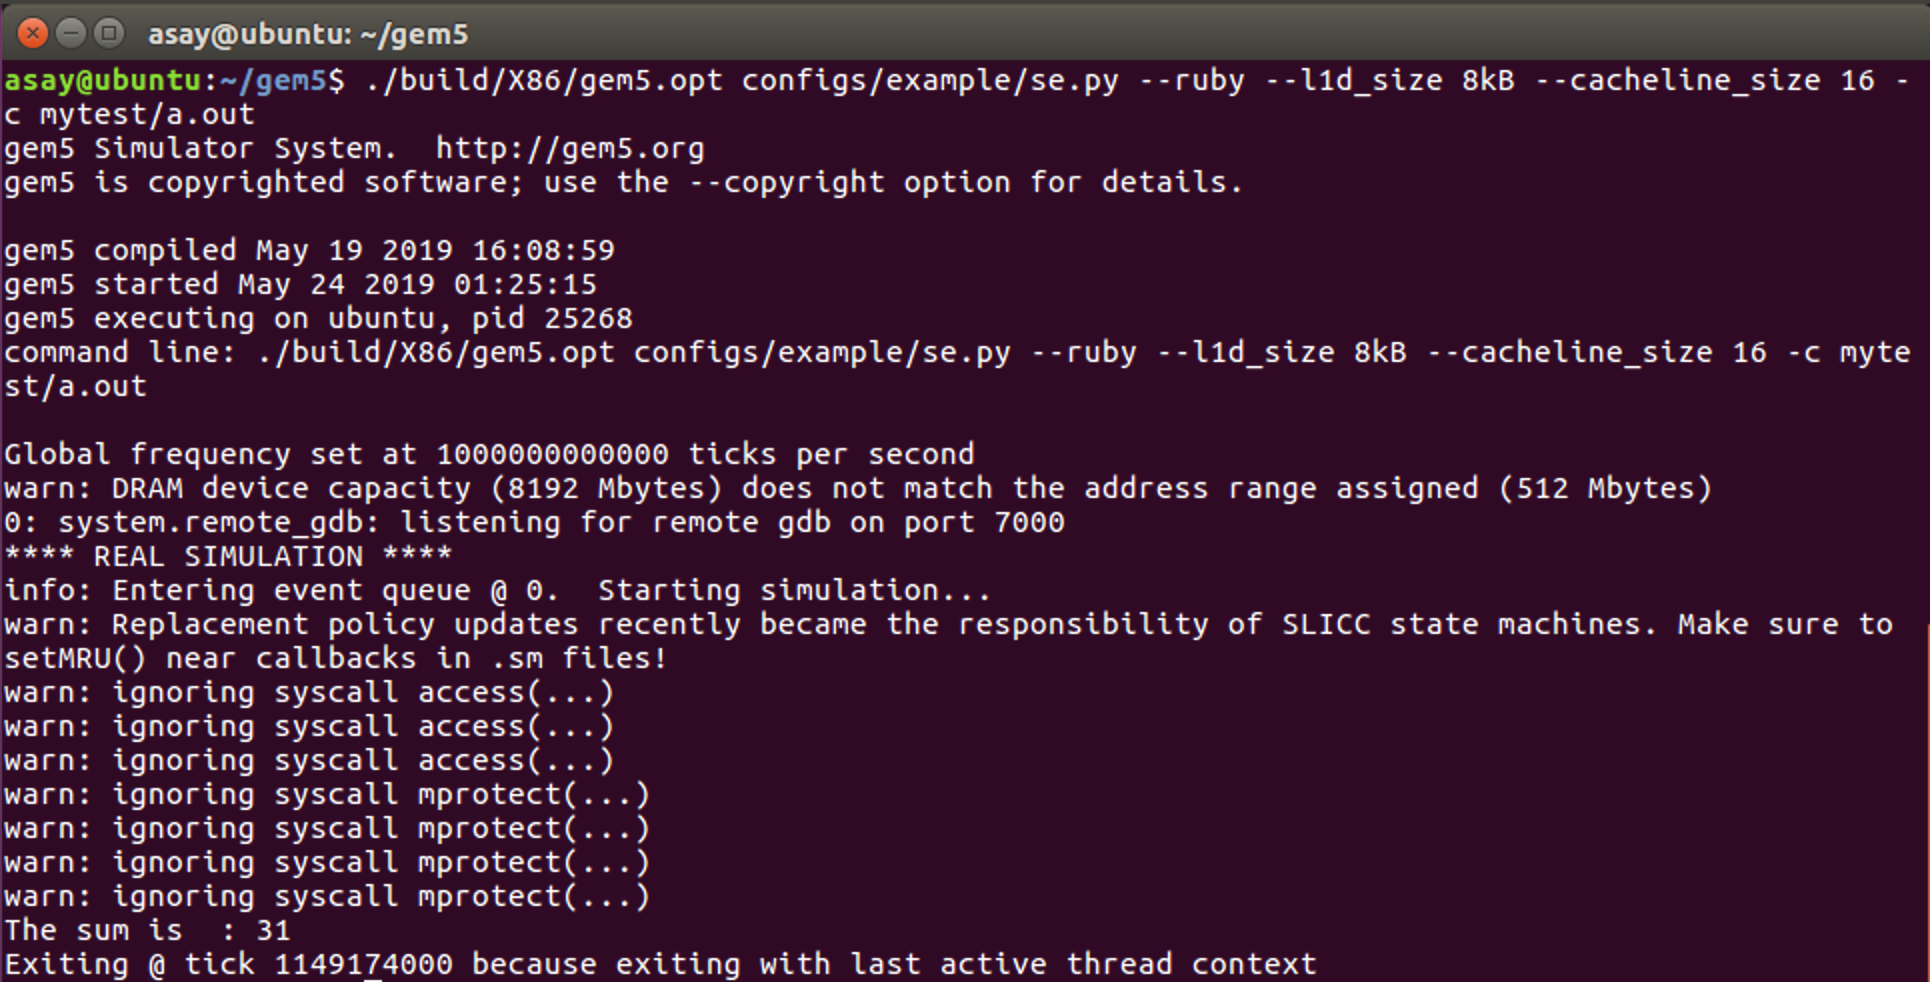
\includegraphics[width=1\textwidth]{816}
\end{center}
\subsection*{\lr{Cachesize = 8kb , cacheline : 32}}
\begin{center}
	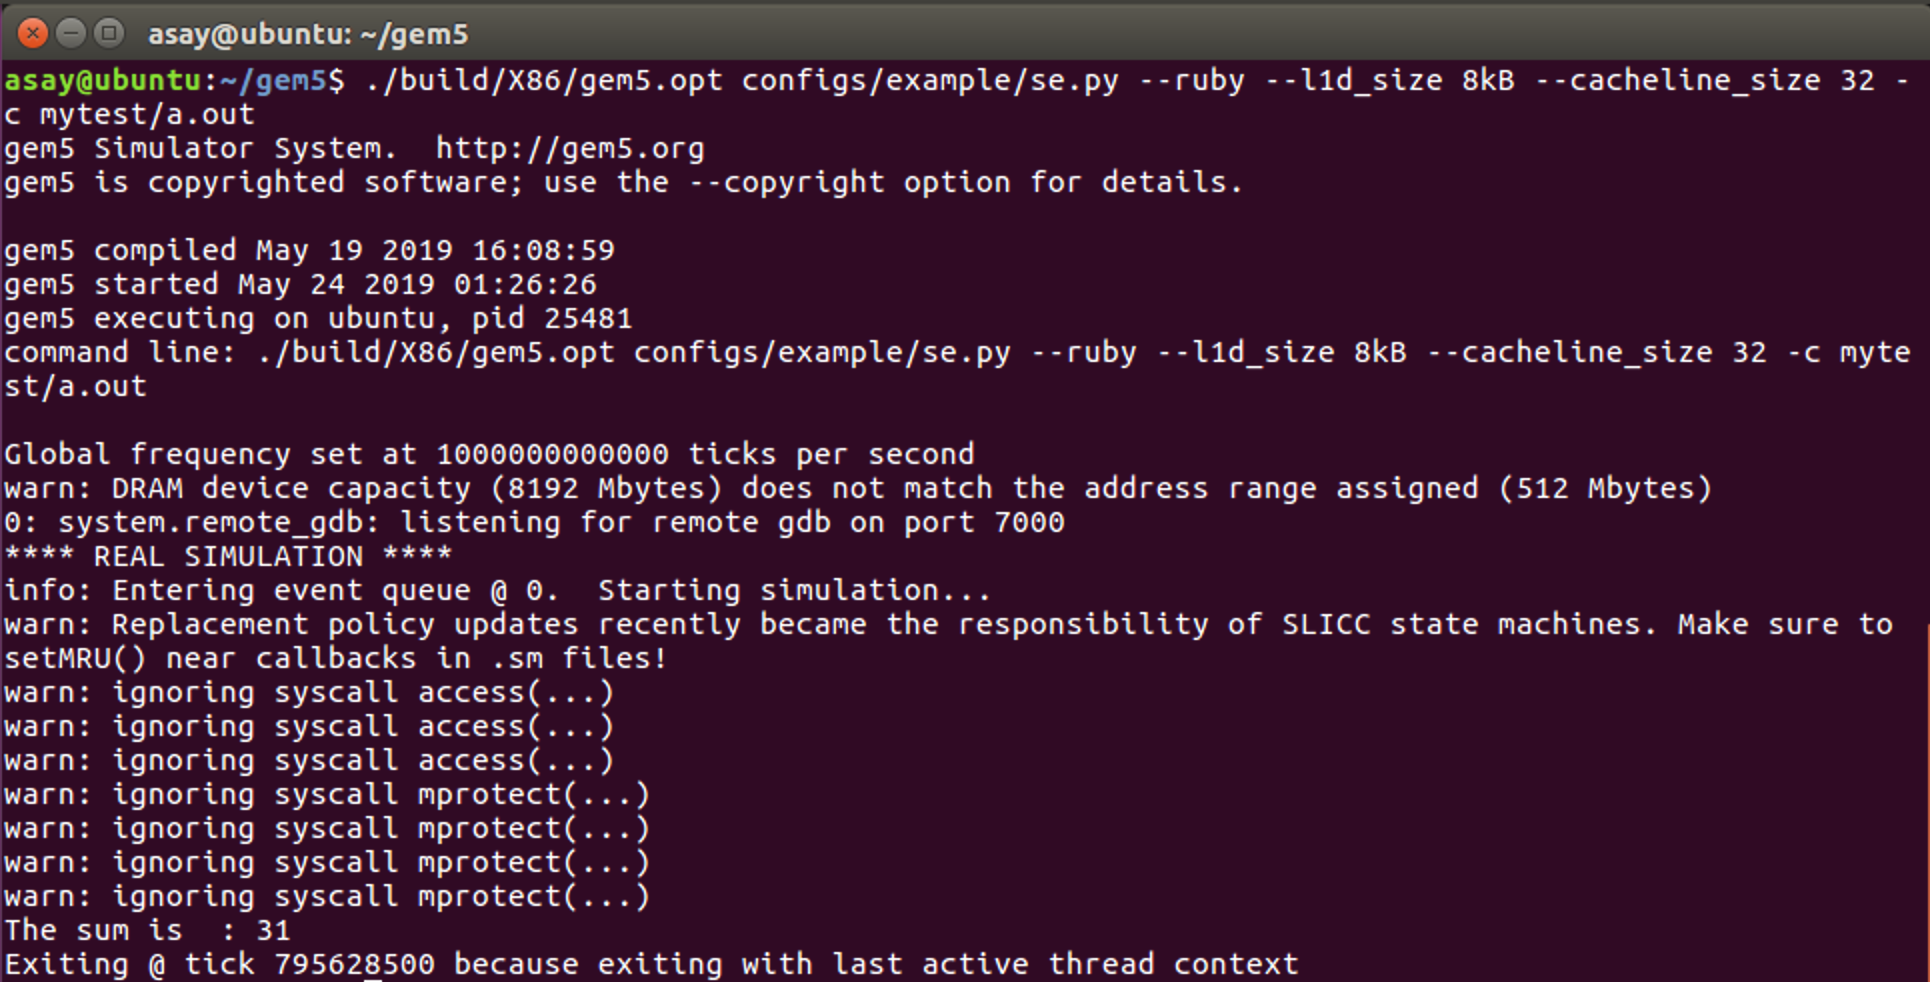
\includegraphics[width=1\textwidth]{832}
\end{center}
\subsection*{\lr{Cachesize = 8kb , cacheline : 64}}
\begin{center}
	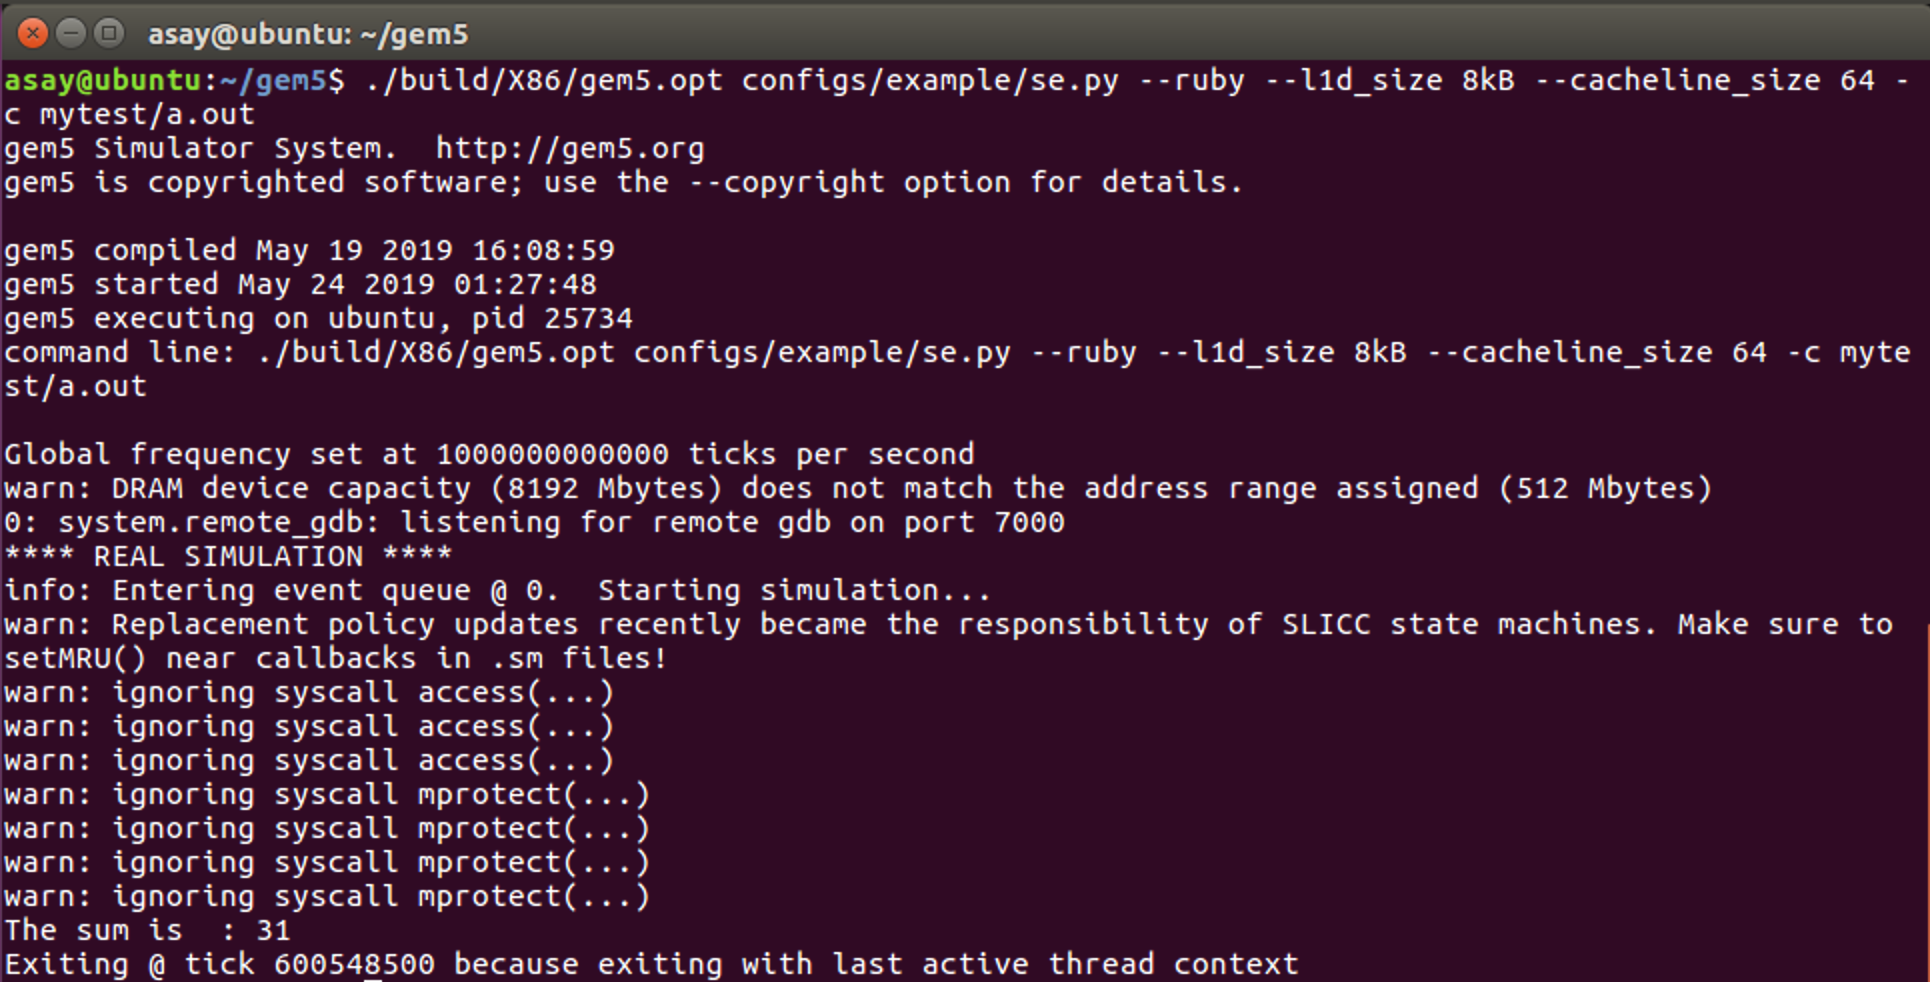
\includegraphics[width=1\textwidth]{864}
\end{center}
\subsection*{\lr{Cachesize = 16kb , cacheline : 16}}
\begin{center}
	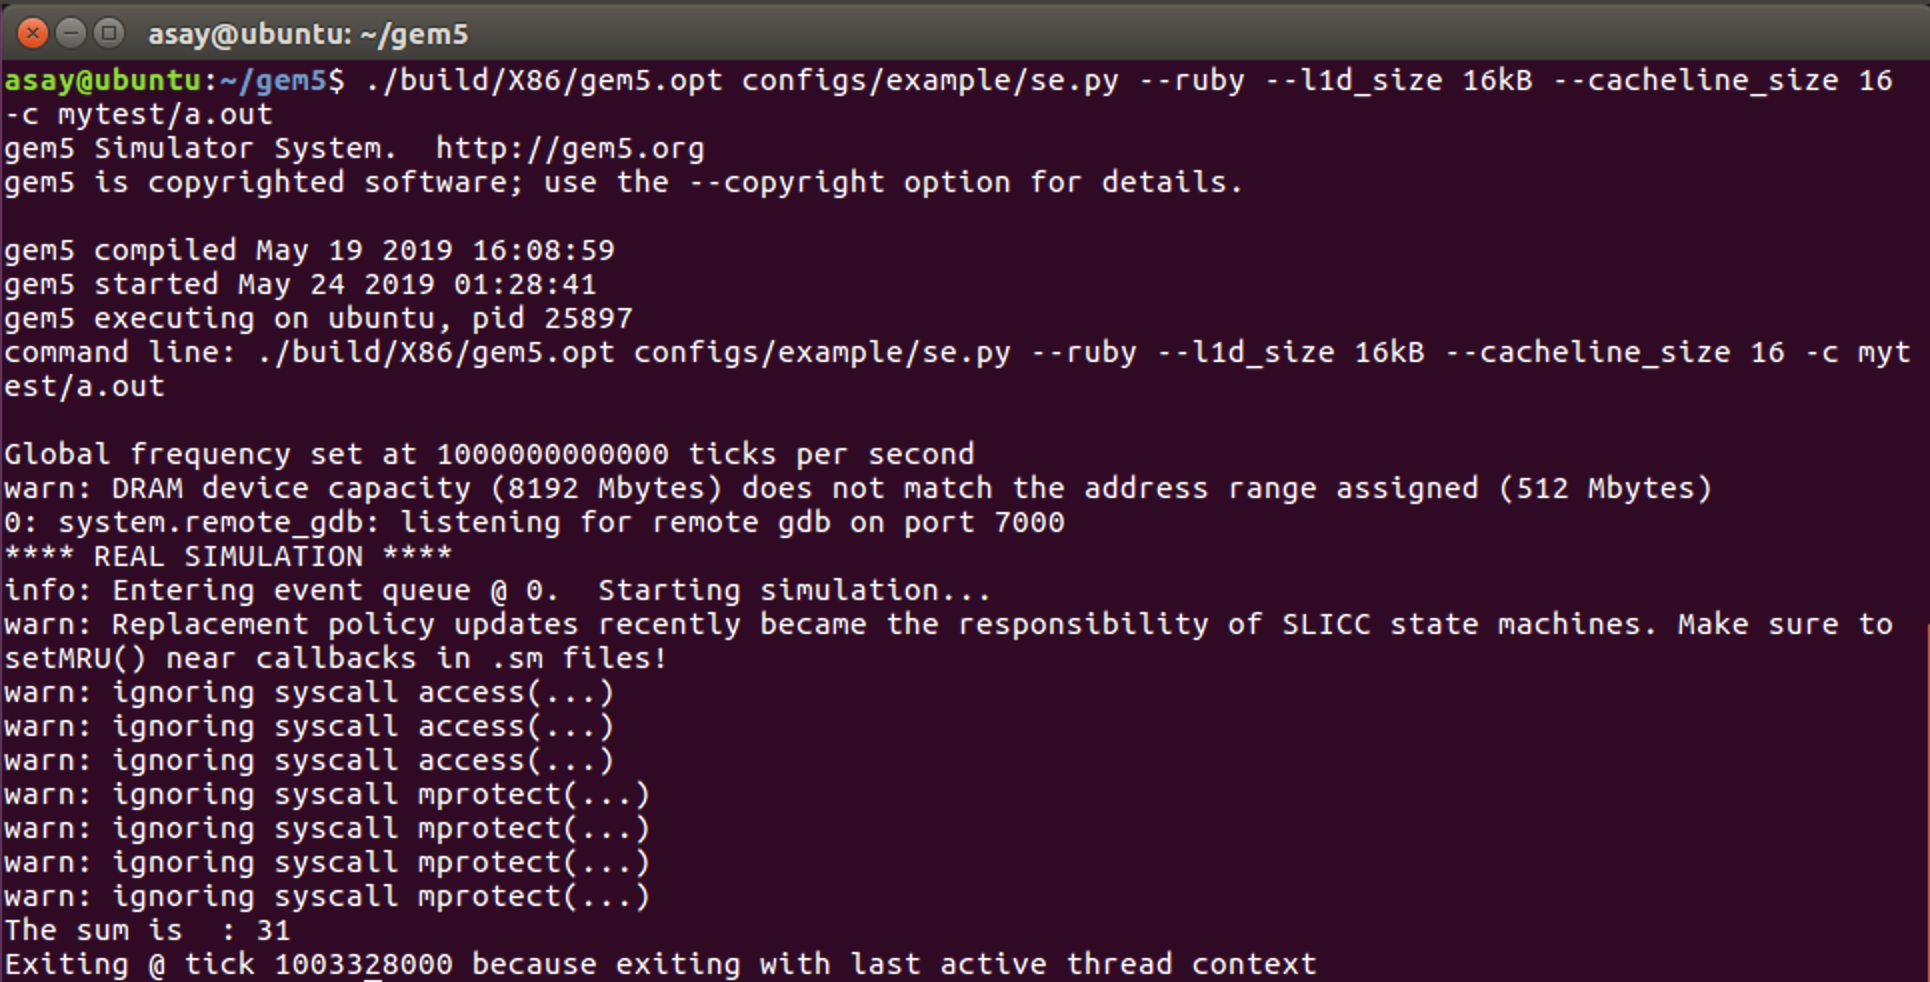
\includegraphics[width=1\textwidth]{1616}
\end{center}
\subsection*{\lr{Cachesize = 16kb , cacheline : 32}}
\begin{center}
	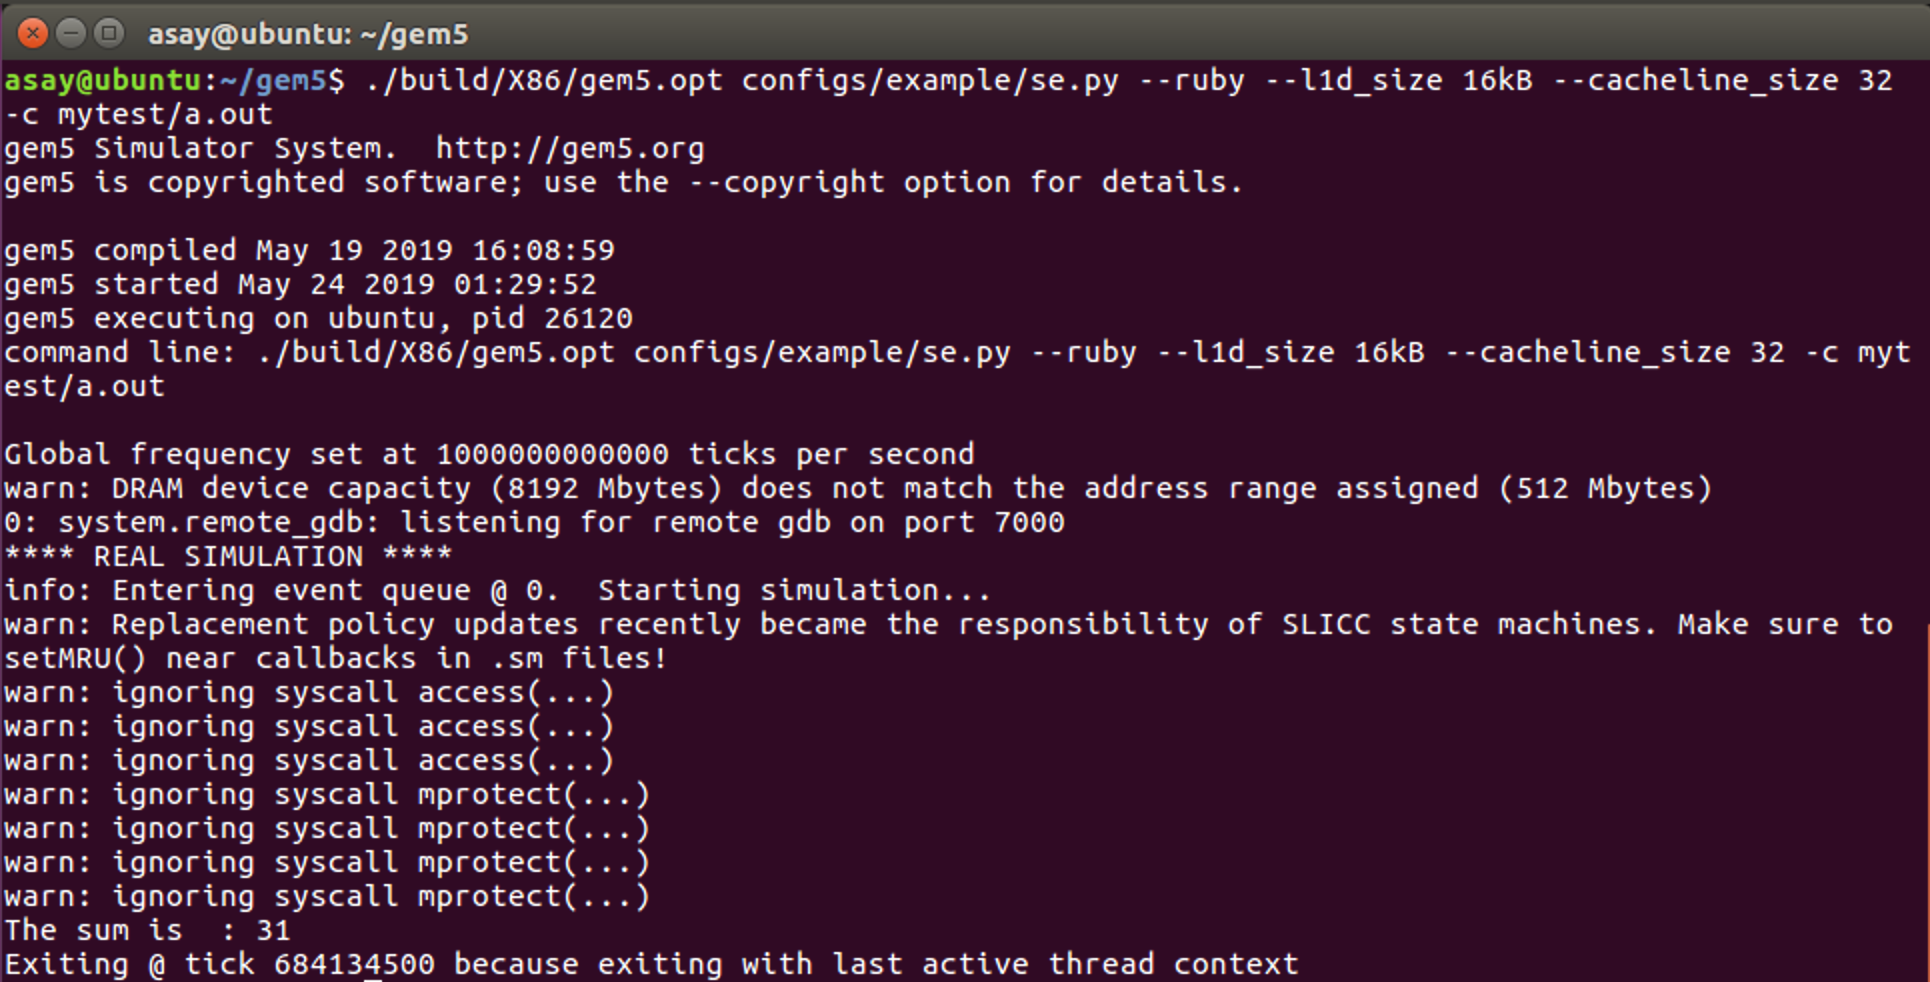
\includegraphics[width=1\textwidth]{1632}
\end{center}
\subsection*{\lr{Cachesize = 16kb , cacheline : 64}}
\begin{center}
	\includegraphics[width=1\textwidth]{1664}
\end{center}
\subsection*{\lr{Cachesize = 32kb , cacheline : 16}}
\begin{center}
	\includegraphics[width=1\textwidth]{1664}
\end{center}
\subsection*{\lr{Cachesize = 32kb , cacheline : 32}}
\begin{center}
	\includegraphics[width=1\textwidth]{3232}
\end{center}
\subsection*{\lr{Cachesize = 32kb , cacheline : 64}}
\begin{center}
	\includegraphics[width=1\textwidth]{3232}
\end{center}
\subsection*{\lr{Cachesize = 64kb , cacheline : 16}}
\begin{center}
	\includegraphics[width=1\textwidth]{6416}
\end{center}
\subsection*{\lr{Cachesize = 64kb , cacheline : 32}}
\begin{center}
	\includegraphics[width=1\textwidth]{6432}
\end{center}
\subsection*{\lr{Cachesize = 64kb , cacheline : 64}}
\begin{center}
	\includegraphics[width=1\textwidth]{6464}
\end{center}

\end{document}